% ==================================================================
%  徐森林、薛春华《数学分析》（第一册）
%  第 1 章  数列极限
%  源：原书印刷页 1-80（PDF 物理页 = 印刷页 + 6）
% ==================================================================

\chapter{数列极限}\label{ch:1}

数学分析主要的研究对象是实变量的一元或多元函数. 众所周知, 正负十进位有限小数与无限循环小数 (即正负分数) 称为有理数; 无限不循环小数称为无理数. 由反证法可知 $\sqrt{2}$, $0.1010010001\cdots$ 均为无理数. 有理数与无理数统称为实数. 有理数的全体称为有理数集. 由代数学的知识知, 它关于通常的加法、乘法具有结合律、交换律与分配律, 并成为一个域, 称为有理数域, 记为 $\mathbb{Q}$. 实数的全体称为实数集, 它关于通常的加法、乘法具有结合律、交换律与分配律, 并成为一个域, 称为实数域, 记为 $\mathbb{R}$.

19 世纪建立的极限理论包括数列极限与函数极限. 极限理论是微分学、积分学的根本, 是数学分析的基础, 也是入数学分析之门的关键. 本章先引进数列极限的概念, 用大量具体的、典型的数列实例, 使读者熟悉 $\varepsilon\text{-}N$ 法及证明数列极限的各种方法. 然后, 在第 2 章中研究函数极限的 $\varepsilon\text{-}\delta$ 法及其重要的性质. 本章还证明了实数连续性的七个等价命题. 实数连续性与数学分析的每一概念都有十分密切的关系, 而且还是不可缺少的理论基础. 它的证明方法也将贯穿整个数学分析的学习过程并延续到分析数学的其他分支中.

% ==================================================================
%  徐森林、薛春华《数学分析》（第一册）
%  \S1.1  数列极限的概念
%  源：原书印刷页 1-14（PDF 物理页 7-20）
% ==================================================================
\section{数列极限的概念}\label{sec:1.1}

依次排列着的一列实数 $a_{1}, a_{2}, \cdots, a_{n}, \cdots$, 称为一个实数列或数列, $a_{n}$ 称为该数列的第 $n$ 项或通项. 记此数列为 $\{a_{n}\}$, 简记为 $a_{n}$.

数列实际上可视作一个实值函数或特殊映射
\[
  f: \mathbb{N} = \{1, 2, \cdots, n, \cdots\} \to \mathbb{R},\quad n \mapsto f(n) = a_n.
\]

考察下列数列 $\{a_{n}\}$ 可以看出, 当项数 $n$ 无限增大时, 有些数列会有一个趋向 (定数 $a$, 或 $+\infty$, 或 $-\infty$, 或 $\infty$), 有些则无这种趋向. 为区别这种现象, 定义极限概念如下: 如果当 $n$ 趋于 $+\infty$ 时, $\{a_{n}\}$ 趋于实数 $a$ ($+\infty$, $-\infty$, $\infty$), 则称 $a$ ($+\infty$, $-\infty$, $\infty$) 为 $\{a_{n}\}$ 的极限, 记作 $\lim_{n\to+\infty}a_{n}=a$ ($+\infty$, $-\infty$, $\infty$). 否则, 称 $\{a_{n}\}$ 无极限.
\begin{align*}
  &\left\{\frac{1}{n}\right\}: 1, \frac{1}{2}, \cdots, \frac{1}{n}, \cdots,\quad \lim_{n\to+\infty}\frac{1}{n}=0;\\
  &\left\{\frac{(-1)^{n-1}}{n}\right\}: 1, -\frac{1}{2}, \cdots, \frac{(-1)^{n-1}}{n}, \cdots,\quad \lim_{n\to+\infty}\frac{(-1)^{n-1}}{n}=0;\\
  &\left\{\frac{n}{n+1}\right\}: \frac{1}{2}, \frac{2}{3}, \cdots, \frac{n}{n+1}, \cdots,\quad \lim_{n\to+\infty}\frac{n}{n+1}=1;\\
  &\left\{\frac{1}{2^{n}}\right\}: \frac{1}{2}, \frac{1}{2^{2}}, \cdots, \frac{1}{2^{n}}, \cdots,\quad \lim_{n\to+\infty}\frac{1}{2^{n}}=0;\\
  &\{n\}: 1, 2, \cdots, n, \cdots,\quad \lim_{n\to+\infty}n=+\infty;\\
  &\{-n\}: -1, -2, \cdots, -n, \cdots,\quad \lim_{n\to+\infty}(-n)=-\infty;\\
  &\left\{(-1)^{n-1}n\right\}: 1, -2, 3, -4, \cdots, (-1)^{n-1}n, \cdots,\quad \lim_{n\to+\infty}(-1)^{n-1}n=\infty;\\
  &\left\{(-1)^{n}\right\}: -1, 1, -1, 1, \cdots,\quad \text{无极限}.
\end{align*}

以上所举数列有无极限, 极限是什么, 一眼就能看出, 但是大多数是无法看出的. 例如, 数列 $\left\{(1+\frac{1}{n})^{n}\right\}$ 有无极限, 极限是什么, 不易确定. 因此, 必须对数列的极限给出确切的定义.

\begin{definition}[$\varepsilon\text{-}N$ 法]\label{def:1.1.1}
设 $\{a_{n}\}$ 为实数列, $a$ 为实数. 如果对任意给定的正数 $\varepsilon$ ($\forall\varepsilon>0$), 总有自然数 $N = N(\varepsilon)$ ($\exists N=N(\varepsilon)\in\mathbb{N}$), 当 $n>N$ 时, 有
\[
  |a_{n}-a|<\varepsilon,\quad \text{即}\ a-\varepsilon<a_{n}<a+\varepsilon,
\]
则称 $a$ 为数列 $\{a_n\}$ 的极限, 或称数列 $\{a_n\}$ 以 $a$ 为极限, 或称数列 $\{a_n\}$ 收敛于 $a$. 此时, $\{a_n\}$ 称为收敛数列, 记为 $\lim_{n\to+\infty} a_n = a$ 或 $a_n \to a\ (n \to +\infty)$. 否则称数列 $\{a_n\}$ 发散.
\end{definition}

根据实数理论 (\S1.3), 实数集与实数轴上的点能建立一一对应关系. 于是, 上述定义可几何表述如下: $a_{n}\ (n>N)$ 都在区间 $(a-\varepsilon, a+\varepsilon)$ 内, 而在 $(a-\varepsilon, a+\varepsilon)$ 外至多有 $a_{1}, a_{2}, \cdots, a_{N}$ 中的 $N$ 项 (如图~\ref{fig:1.1.1} 所示).

类似地, 用 $A\text{-}N$ 法得到下列定义:

如果 $\forall A>0,\ \exists N=N(A)\in\mathbb{N}$, 当 $n>N$ 时, 有 $a_{n}>A$, 则称 $+\infty$ 为数列 $\{a_{n}\}$ 的极限, 或称 $\{a_{n}\}$ 以 $+\infty$ 为极限, 或 $\{a_{n}\}$ 发散于 $+\infty$, 记为 $\lim_{n\to+\infty}a_{n}=+\infty$ 或 $a_{n}\to+\infty\ (n\to+\infty)$. 此时, 在 $(A,+\infty)$ 外至多有 $a_{1},\cdots,a_{N}$ 中的 $N$ 项 (如图~\ref{fig:1.1.2} 所示).

\begin{figure}[htbp]
\centering
\begin{minipage}[t]{0.48\textwidth}
\centering
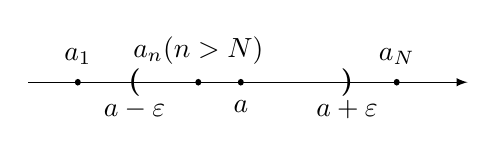
\begin{tikzpicture}[>=latex, xscale=0.9]
  \draw[->] (-3,0) -- (3.2,0);
  \node[above] at (-2.3,0.1) {$a_1$};
  \fill (-2.3,0) circle (1.2pt);
  \node at (-1.5,0) {\textbf{(}};
  \node[below=3pt] at (-1.5,0) {$a-\varepsilon$};
  \node[above] at (-0.6,0.1) {$a_n(n>N)$};
  \fill (-0.6,0) circle (1.2pt);
  \fill (0,0) circle (1.2pt);
  \node[below=3pt] at (0,0) {$a$};
  \node at (1.5,0) {\textbf{)}};
  \node[below=3pt] at (1.5,0) {$a+\varepsilon$};
  \node[above] at (2.2,0.1) {$a_N$};
  \fill (2.2,0) circle (1.2pt);
\end{tikzpicture}
\caption{}\label{fig:1.1.1}
\end{minipage}
\hfill
\begin{minipage}[t]{0.48\textwidth}
\centering
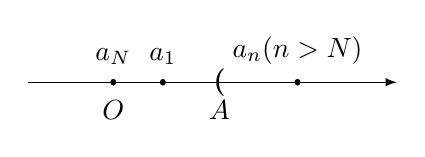
\begin{tikzpicture}[>=latex, xscale=0.9]
  \draw[->] (-1.2,0) -- (4,0);
  \fill (0,0) circle (1.2pt);
  \node[below=3pt] at (0,0) {$O$};
  \node[above] at (0,0.1) {$a_N$};
  \fill (0.7,0) circle (1.2pt);
  \node[above] at (0.7,0.1) {$a_1$};
  \node at (1.5,0) {\textbf{(}};
  \node[below=3pt] at (1.5,0) {$A$};
  \fill (2.6,0) circle (1.2pt);
  \node[above] at (2.6,0.1) {$a_n(n>N)$};
\end{tikzpicture}
\caption{}\label{fig:1.1.2}
\end{minipage}
\end{figure}

如果 $\forall A>0,\ \exists N=N(A)\in\mathbb{N}$, 当 $n>N$ 时, 有 $a_{n}<-A$, 则称 $-\infty$ 为数列 $\{a_{n}\}$ 的极限, 或称 $\{a_{n}\}$ 以 $-\infty$ 为极限, 或 $\{a_{n}\}$ 发散于 $-\infty$, 记为 $\lim_{n\to+\infty}a_{n}=-\infty$ 或 $a_{n}\to-\infty\ (n\to+\infty)$. 此时, 在 $(-\infty,-A)$ 外至多有 $a_{1},\cdots,a_{N}$ 中的 $N$ 项 (如图~\ref{fig:1.1.3} 所示).

如果 $\forall A>0,\ \exists N=N(A)\in\mathbb{N}$, 当 $n>N$ 时, 有
\[
  |a_{n}|>A,
\]
则称 $\infty$ 为数列 $\{a_{n}\}$ 的极限, 或称 $\{a_{n}\}$ 以 $\infty$ 为极限, 或 $\{a_{n}\}$ 发散于 $\infty$, 记为 $\lim_{n\to+\infty}a_{n}=\infty$ 或 $a_{n}\to\infty\ (n\to+\infty)$. 此时, 在 $(-\infty,-A)\cup(A,+\infty)$ 外, 即 $[-A,A]$ 中至多有 $a_{1},\cdots,a_{N}$ 中的 $N$ 项 (如图~\ref{fig:1.1.4} 所示).

\begin{figure}[htbp]
\centering
\begin{minipage}[t]{0.48\textwidth}
\centering
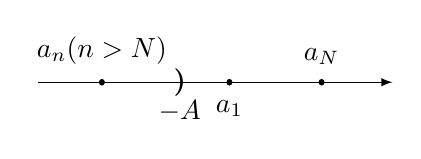
\begin{tikzpicture}[>=latex, xscale=0.9]
  \draw[->] (-3.5,0) -- (1.5,0);
  \fill (-2.6,0) circle (1.2pt);
  \node[above] at (-2.6,0.1) {$a_n(n>N)$};
  \node at (-1.5,0) {\textbf{)}};
  \node[below=3pt] at (-1.5,0) {$-A$};
  \fill (-0.8,0) circle (1.2pt);
  \node[below=3pt] at (-0.8,0) {$a_1$};
  \fill (0.5,0) circle (1.2pt);
  \node[above] at (0.5,0.1) {$a_N$};
\end{tikzpicture}
\caption{}\label{fig:1.1.3}
\end{minipage}
\hfill
\begin{minipage}[t]{0.48\textwidth}
\centering
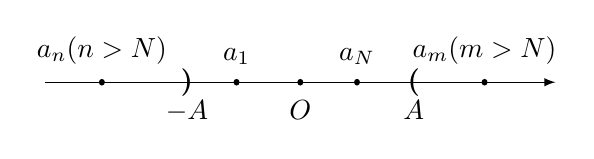
\begin{tikzpicture}[>=latex, xscale=0.9]
  \draw[->] (-3.6,0) -- (3.6,0);
  \fill (-2.8,0) circle (1.2pt);
  \node[above] at (-2.8,0.1) {$a_n(n>N)$};
  \node at (-1.6,0) {\textbf{)}};
  \node[below=3pt] at (-1.6,0) {$-A$};
  \fill (-0.9,0) circle (1.2pt);
  \node[above] at (-0.9,0.1) {$a_1$};
  \fill (0,0) circle (1.2pt);
  \node[below=3pt] at (0,0) {$O$};
  \fill (0.8,0) circle (1.2pt);
  \node[above] at (0.8,0.1) {$a_N$};
  \node at (1.6,0) {\textbf{(}};
  \node[below=3pt] at (1.6,0) {$A$};
  \fill (2.6,0) circle (1.2pt);
  \node[above] at (2.6,0.1) {$a_m(m>N)$};
\end{tikzpicture}
\caption{}\label{fig:1.1.4}
\end{minipage}
\end{figure}

综合上述各种情况可知, 一个数列 $\{a_n\}$ 或者收敛 (即 $\lim_{n\to+\infty}a_n=a\in\mathbb{R}$), 或者发散 (即 $\lim_{n\to+\infty}a_n=+\infty, -\infty, \infty$ 或无极限).

显然, 改变数列 $\{a_{n}\}$ 的有限多项, 或去掉有限多项, 或添加有限多项, 不会改变数列 $\{a_{n}\}$ 的收敛和发散性.

\begin{example}\label{ex:1.1.1}
对常数列 $\{a_{n}\}$, $a_{n} = a$, 有 $\lim_{n \to +\infty} a_{n} = \lim_{n \to +\infty} a = a$.
\end{example}
\begin{proof}
$\forall\varepsilon>0$, 取任意的自然数 $N$, 当 $n>N$ 时, 有
\[
  |a_{n}-a|=|a-a|=0<\varepsilon,
\]
所以 $\lim_{n\to+\infty}a_n=\lim_{n\to+\infty}a=a$.
\end{proof}

\begin{example}\label{ex:1.1.2}
$\lim_{n\to+\infty}\frac{1}{n^\alpha}=0\ (\alpha>0)$.
\end{example}
\begin{proof}
$\forall\varepsilon>0$, 取 $N\in\mathbb{N}$, s.\,t. (such that, 使得) $N>\left(\frac{1}{\varepsilon}\right)^{\frac{1}{\alpha}}$ 或者 $N=\left[\left(\frac{1}{\varepsilon}\right)^{\frac{1}{\alpha}}\right]+1$ (其中 $[x]$ 表示不超过 $x$ 的最大整数), 当 $n>N$ 时, 有
\[
  \left|\frac{1}{n^{\alpha}}-0\right|=\frac{1}{n^{\alpha}}<\frac{1}{N^{\alpha}}<\varepsilon,
\]
所以 $\lim_{n\to+\infty}\frac{1}{n^{\alpha}}=0$.

当 $\alpha=1$ 时, $\lim_{n\to+\infty}\frac{1}{n}=0$, 取 $N=\left[\frac{1}{\varepsilon}\right]+1$ (或 $N>\frac{1}{\varepsilon}, N\in\mathbb{N}$).
\end{proof}

\begin{example}\label{ex:1.1.3}
$\lim_{n\to+\infty}q^n=0\ (|q|<1)$.
\end{example}
\begin{proof}
\textit{证法 1}\quad 当 $0<|q|<1$ 时, $\frac{1}{|q|}>1$, 可设 $\frac{1}{|q|}=1+h\ (h>0)$. $\forall\varepsilon>0$, 取 $N\in\mathbb{N}$, s.\,t. $N>\frac{1}{\varepsilon h}$, 当 $n>N$ 时, 由二项式展开式知
\[
  \frac{1}{|q|^n}=(1+h)^n = 1+nh+\cdots+h^n > nh > Nh > \frac{1}{\varepsilon},
\]
即 $|q^n| < \varepsilon$. 于是
\[
  |q^n-0|=|q^n|<\varepsilon,
\]
所以 $\lim_{n\to+\infty}q^{n}=0$.

当 $q=0$ 时, 由例~\ref{ex:1.1.1} 知, $\lim_{n\to+\infty}q^{n}=\lim_{n\to+\infty}0=0$.

\textit{证法 2}\quad 当 $0<|q|<1$ 时, $\forall\varepsilon>0$, 取 $N\in\mathbb{N}$, s.\,t. $N>\log_{|q|}\varepsilon$, 当 $n>N$ 时, 有
\[
  |q^{n}-0|=|q^{n}|<|q|^{N}<\varepsilon,
\]
所以 $\lim_{n\to+\infty}q^n=0$.
\end{proof}

\begin{example}\label{ex:1.1.4}
证明:
\begin{enumerate}
  \item 当 $q>1$ 时, $\lim_{n\to+\infty}q^n=+\infty$;
  \item 当 $q<-1$ 时, $\lim_{n\to+\infty}q^n=\infty$;
  \item 当 $q=-1$ 时, 数列 $\{q^n\}$ 无极限.
\end{enumerate}
\end{example}
\begin{proof}
(1) 设 $q=1+h\ (h>0)$. $\forall A>0$, 取 $N\in\mathbb{N}$, s.\,t. $N>\frac{A}{h}$. 当 $n>N$ 时, 由二项式定理有
\[
  q^n=(1+h)^n = 1+nh+\cdots+h^n > nh > Nh > A,
\]
所以 $\lim_{n\to+\infty}q^n=+\infty$.

(2) 当 $q<-1$ 时, $|q|>1$. 仿 (1) 可证 $\lim_{n\to+\infty}|q|^n=+\infty$, 即 $\forall A>0,\ \exists N\in\mathbb{N}$, 当 $n>N$ 时, 有 $|q^n|=|q|^n>A$. 因此 $\lim_{n\to+\infty}q^n=\infty$.

(3) 此外, 当 $|q|<1$ 时, 由例~\ref{ex:1.1.3} 知 $\lim_{n\to+\infty}q^n=0$; 当 $q=1$ 时, 由例~\ref{ex:1.1.1} 知 $\lim_{n\to+\infty}q^n=\lim_{n\to+\infty}1=1$; 最后, 当 $q=-1$ 时, 由后面的例~\ref{ex:1.1.12} 推得 $\lim_{n\to+\infty}q^n$ 不存在.
\end{proof}

\begin{example}\label{ex:1.1.5}
设 $a$ 为实常数, 则 $\lim_{n\to+\infty}\frac{a^n}{n!}=0$.
\end{example}
\begin{proof}
显然, $\exists N_{0} \in \mathbb{N}$, s.\,t. $N_{0}>2|a|$, 即 $\frac{|a|}{N_0}<\frac{1}{2}$. 当 $n>N_0$ 时,
\begin{align*}
  \left|\frac{a^{n}}{n!}-0\right| &= \frac{|a|^{n}}{n!} = \frac{|a|}{1}\cdot\frac{|a|}{2}\cdots\frac{|a|}{N_{0}}\cdot\frac{|a|}{N_{0}+1}\cdots\frac{|a|}{n}\\
  &< \frac{|a|^{N_{0}}}{N_{0}!}\left(\frac{|a|}{N_{0}}\right)^{n-N_{0}} < \frac{|a|^{N_{0}}}{N_{0}!}\left(\frac{1}{2}\right)^{n-N_{0}} = C\left(\frac{1}{2}\right)^{n},
\end{align*}
其中 $C = \frac{|a|^{N_0}}{N_0!}\cdot 2^{N_0}$ 为与 $n$ 无关的常数.

由例~\ref{ex:1.1.3} 知, $\lim_{n\to+\infty}\left(\frac{1}{2}\right)^{n}=0$. 故 $\forall\varepsilon>0,\ \exists N_{1}\in\mathbb{N}$, 当 $n>N_1$ 时, 有 $\left(\frac{1}{2}\right)^{n}<\frac{\varepsilon}{C}$. 取 $N=\max\{N_0, N_1\}$, 当 $n>N$ 时, 有
\[
  \left|\frac{a^n}{n!}-0\right| < C\left(\frac{1}{2}\right)^n < C\cdot\frac{\varepsilon}{C}=\varepsilon,
\]
所以 $\lim_{n\to+\infty}\frac{a^n}{n!}=0$.
\end{proof}

\begin{example}\label{ex:1.1.6}
$\lim_{n\to+\infty}\sqrt[n]{a}=\lim_{n\to+\infty}a^{\frac{1}{n}}=1\ (a>0)$.
\end{example}
\begin{proof}
\textit{证法 1}\quad 当 $a=1$ 时, 由例~\ref{ex:1.1.1} 可知 $\lim_{n\to+\infty}\sqrt[n]{a}=\lim_{n\to+\infty}1=1$.

当 $a>1$ 时, $\sqrt[n]{a}>1$. 令 $\sqrt[n]{a}=1+\alpha_n\ (\alpha_n>0)$, 则
\[
  a = (1+\alpha_n)^n = 1+n\alpha_n+\cdots+\alpha_n^n > n\alpha_n,
\]
即 $0<\alpha_n<\frac{a}{n}$. $\forall\varepsilon>0$, 取 $N>\left[\frac{a}{\varepsilon}\right]$, 当 $n>N$ 时, 有
\[
  |\sqrt[n]{a}-1| = \alpha_n < \frac{a}{n} < \frac{a}{N} < \varepsilon,
\]
所以 $\lim_{n\to+\infty}\sqrt[n]{a}=1$.

当 $0<a<1$ 时, $\frac{1}{a}>1$. 由上面已证的结果, $\lim_{n\to+\infty}\sqrt[n]{\frac{1}{a}}=1$, 从而
\[
  \lim_{n\to+\infty}\sqrt[n]{a}=\lim_{n\to+\infty}\frac{1}{\sqrt[n]{\frac{1}{a}}}=1.
\]

\textit{证法 2}\quad 当 $a>1$ 时, $\forall\varepsilon>0$, 只要取 $N\in\mathbb{N}$, s.\,t. $N>\log_{1+\varepsilon}a$, 当 $n>N$ 时, 便有
\[
  1 \leqslant \sqrt[n]{a} < \sqrt[N]{a} < 1+\varepsilon,
\]
即 $|\sqrt[n]{a}-1|<\varepsilon$. 故 $\lim_{n\to+\infty}\sqrt[n]{a}=1$. $a\leqslant 1$ 的情形同证法 1.
\end{proof}

\begin{example}\label{ex:1.1.7}
$\lim_{n\to+\infty}\sqrt[n]{n}=1$.
\end{example}
\begin{proof}
\textit{证法 1}\quad 令 $\sqrt[n]{n}=1+\alpha_{n}\ (\alpha_{n}\geqslant0)$, 则当 $n>1$ 时,
\[
  n = (1+\alpha_{n})^{n} = 1+n\alpha_{n}+\frac{n(n-1)}{2}\alpha_{n}^{2}+\cdots+\alpha_{n}^{n} > \frac{n(n-1)}{2}\alpha_{n}^{2},
\]
从而 $\alpha_n^2 < \frac{2}{n-1}$, 即 $0 \leqslant \alpha_n < \sqrt{\frac{2}{n-1}}$.

$\forall\varepsilon>0$, 取 $N = \left[\frac{2}{\varepsilon^2}\right]+1$, 当 $n>N$ 时, 有
\[
  |\sqrt[n]{n}-1| = \alpha_n < \sqrt{\frac{2}{n-1}} < \sqrt{\frac{2}{N-1}} \leqslant \varepsilon,
\]
所以 $\lim_{n\to+\infty}\sqrt[n]{n}=1$.

\textit{证法 2}\quad $\forall\varepsilon>0$, 取充分大的自然数 $k$, 使 $(1+\varepsilon)^k > 2$. 当 $n>2^k$ 时,
\[
  1 \leqslant \sqrt[n]{n} < \sqrt[n]{(1+\varepsilon)^n} = 1+\varepsilon,
\]
所以 $\lim_{n\to+\infty}\sqrt[n]{n}=1$.
\end{proof}

\begin{example}\label{ex:1.1.8}
设 $a_{n}=0.\underbrace{33\cdots3}_n$, 则 $\lim_{n\to+\infty}a_{n}=\frac{1}{3}$.
\end{example}
\begin{proof}
因为
\[
  a_{n} = \frac{3}{10}+\frac{3}{10^2}+\cdots+\frac{3}{10^n} = \frac{\frac{3}{10}\left(1-\frac{1}{10^n}\right)}{1-\frac{1}{10}} = \frac{1}{3}\left(1-\frac{1}{10^n}\right),
\]
所以
\[
  \left|a_{n}-\frac{1}{3}\right| = \frac{1}{3\cdot 10^n} < \frac{1}{10^n}.
\]
$\forall\varepsilon>0$, 取 $N = \left[\lg\frac{1}{\varepsilon}\right]+1$, 当 $n>N$ 时, 有
\[
  \left|a_{n}-\frac{1}{3}\right| < \frac{1}{10^n} < \frac{1}{10^N} \leqslant \varepsilon,
\]
所以 $\lim_{n\to+\infty}a_{n}=\frac{1}{3}$.
\end{proof}

\begin{example}\label{ex:1.1.9}
$\lim_{n \to +\infty} \frac{1}{n \sqrt[n]{n!}} = 0$.
\end{example}
\begin{proof}
\textit{证法 1}\quad $\forall\varepsilon>0$, 由例~\ref{ex:1.1.5} 知 $\lim_{n\to+\infty}\frac{(1/\varepsilon)^n}{n!}=0$. 故 $\exists N\in\mathbb{N}$, 当 $n>N$ 时, 有
\[
  \frac{(1/\varepsilon)^{n}}{n!}<1,
\]
所以
\[
  -\varepsilon < 0 < \frac{1}{\sqrt[n]{n!}} < \varepsilon,
\]
即 $\lim_{n\to+\infty}\frac{1}{\sqrt[n]{n!}}=0$. 进而由 $n\geqslant 1$ 知
\[
  0 < \frac{1}{n\sqrt[n]{n!}} \leqslant \frac{1}{\sqrt[n]{n!}} < \varepsilon,
\]
所以 $\lim_{n\to+\infty}\frac{1}{n\sqrt[n]{n!}}=0$.

\textit{证法 2}\quad 容易验证不等式 $n! > \left(\frac{n}{e}\right)^n$ (可参阅例~\ref{ex:1.4.11}). 从而
\[
  0 < \frac{1}{n\sqrt[n]{n!}} < \frac{e}{n^2}.
\]
$\forall\varepsilon>0$, 取 $N = \left[\sqrt{\frac{e}{\varepsilon}}\right]+1$, 当 $n>N$ 时即有 $\frac{e}{n^2}<\varepsilon$, 故极限为 0.
\end{proof}

\begin{example}\label{ex:1.1.10}
$\lim_{n\to+\infty}\frac{3n^{2}}{n^{2}-3}=3$.
\end{example}
\begin{proof}
当 $n\geqslant 2$ 时, $n^2-3 > \frac{n^2}{2}$. 故
\[
  \left|\frac{3n^{2}}{n^{2}-3}-3\right| = \frac{9}{n^{2}-3} < \frac{18}{n^{2}}.
\]
$\forall\varepsilon>0$, 取 $N = \max\left\{2, \left[\sqrt{\frac{18}{\varepsilon}}\right]+1\right\}$, 当 $n>N$ 时, 有
\[
  \left|\frac{3n^{2}}{n^{2}-3}-3\right| < \frac{18}{n^2} < \frac{18}{N^2} \leqslant \varepsilon,
\]
所以 $\lim_{n\to+\infty}\frac{3n^{2}}{n^{2}-3}=3$.
\end{proof}

\begin{example}\label{ex:1.1.11}
$\lim_{n \to +\infty} \frac{3 \sqrt{n} + 1}{2 \sqrt{n} + n} = 0$.
\end{example}
\begin{proof}
$\forall\varepsilon>0$, 当 $n\geqslant 1$ 时,
\[
  \left|\frac{3\sqrt{n}+1}{2\sqrt{n}+n}-0\right| = \frac{3\sqrt{n}+1}{2\sqrt{n}+n} < \frac{4\sqrt{n}}{n} = \frac{4}{\sqrt{n}}.
\]
取 $N = \left[\frac{16}{\varepsilon^2}\right]+1$, 当 $n>N$ 时, 有
\[
  \left|\frac{3\sqrt{n}+1}{2\sqrt{n}+n}-0\right| < \frac{4}{\sqrt{n}} < \frac{4}{\sqrt{N}} \leqslant \varepsilon,
\]
所以 $\lim_{n\to+\infty}\frac{3\sqrt{n}+1}{2\sqrt{n}+n}=0$.
\end{proof}

\begin{theorem}\label{thm:1.1.1}
数列 $\{a_{n}\}$ 有极限 $a$ 的充分必要条件是它的偶数项数列 (偶子列) $\{a_{2k}\}$ 和奇数项数列 (奇子列) $\{a_{2k-1}\}$ 都有极限且极限均为 $a$.
\end{theorem}
\begin{proof}
\textbf{必要性:}\quad 设 $\lim_{n\to+\infty}a_n=a$.

若 $a$ 为有限实数, 则 $\forall\varepsilon>0,\ \exists N\in\mathbb{N}$, 当 $n>N$ 时, 有 $|a_n-a|<\varepsilon$. 特别地, 取自然数 $K = \left[\frac{N}{2}\right]+1$, 当 $k>K$ 时, $2k>2k-1>N$, 因而
\[
  |a_{2k}-a|<\varepsilon\quad \text{与}\quad |a_{2k-1}-a|<\varepsilon,
\]
即 $\lim_{k\to+\infty}a_{2k}=a$ 且 $\lim_{k\to+\infty}a_{2k-1}=a$.

对 $a=+\infty, -\infty, \infty$ 的情形完全类似可证.

\textbf{充分性:}\quad 设 $\lim_{k\to+\infty}a_{2k}=a$ 且 $\lim_{k\to+\infty}a_{2k-1}=a$.

若 $a$ 为有限实数, 则 $\forall\varepsilon>0$, $\exists K_1\in\mathbb{N}$, 当 $k>K_1$ 时, $|a_{2k}-a|<\varepsilon$; $\exists K_2\in\mathbb{N}$, 当 $k>K_2$ 时, $|a_{2k-1}-a|<\varepsilon$. 取 $N = \max\{2K_1, 2K_2-1\}$, 则当 $n>N$ 时, 无论 $n$ 是偶数 ($n=2k>2K_1$) 还是奇数 ($n=2k-1>2K_2-1$), 都有 $|a_n-a|<\varepsilon$. 故 $\lim_{n\to+\infty}a_n=a$.

对 $a=+\infty, -\infty, \infty$ 的情形同理可证.
\end{proof}

下面引进开邻域的概念:
\begin{enumerate}
  \item 设 $a\in\mathbb{R}$, 称开区间 $(a-\varepsilon, a+\varepsilon)$ 为点 $a$ 的 $\varepsilon$ 邻域, 记作 $U(a;\varepsilon)$ 或简记为 $U(a)$. 称集合 $U^\circ(a;\varepsilon) = (a-\varepsilon, a)\cup(a, a+\varepsilon)$ 为点 $a$ 的去心邻域.
  \item 称开区间 $(A, +\infty)$ 为点 $+\infty$ 的开邻域, 记作 $U(+\infty; A)$ 或 $U(+\infty)$.
  \item 称开区间 $(-\infty, -A)$ 为点 $-\infty$ 的开邻域, 记作 $U(-\infty; A)$ 或 $U(-\infty)$.
  \item 称开集 $(-\infty, -A)\cup(A, +\infty)$ 为点 $\infty$ 的开邻域, 记作 $U(\infty; A)$ 或 $U(\infty)$.
\end{enumerate}

由开邻域的概念, 数列极限的定义可以统一叙述为:
\[
  \lim_{n\to+\infty}a_n = a \iff \text{对 } a \text{ 的任何开邻域 } U,\ \exists N\in\mathbb{N},\ \text{当 } n>N \text{ 时, } a_n\in U.
\]

\begin{theorem}\label{thm:1.1.2}
$\lim_{n\to+\infty}a_n=a \iff$ 对 $\{a_n\}$ 的任何子列 $\{a_{n_k}\}$ 都有 $\lim_{k\to+\infty}a_{n_k}=a$.
\end{theorem}
\begin{proof}
\textbf{充分性:}\quad 因为数列 $\{a_n\}$ 本身就是它的一个平凡子列 (取 $n_k=k$), 所以结论显然成立.

\textbf{必要性:}\quad 设 $\lim_{n\to+\infty}a_n=a$. 对 $a$ 的任何开邻域 $U$, $\exists N\in\mathbb{N}$, 当 $n>N$ 时, $a_n\in U$. 因为子列的下标序列 $\{n_k\}$ 严格递增, 且 $n_k\geqslant k$, 所以当 $k>N$ 时必有 $n_k\geqslant k>N$, 从而 $a_{n_k}\in U$. 故 $\lim_{k\to+\infty}a_{n_k}=a$.
\end{proof}

\begin{theorem}\label{thm:1.1.3}
数列 $\{a_{n}\}$ 有极限 (实数 $a$ 或 $+\infty$ 或 $-\infty$) 的充要条件是它的任何非平凡子列都有极限.
\end{theorem}
\begin{proof}
必要性由定理~\ref{thm:1.1.2} 直接保证. 充分性反设 $\{a_n\}$ 没有极限, 则由极限否定定义可析出两个极限不同的子列, 矛盾.
\end{proof}

\begin{theorem}\label{thm:1.1.4}
数列 $\{a_{n}\}$ 收敛 $\iff \{a_{n}\}$ 的任何非平凡子列都收敛.
\end{theorem}

\begin{theorem}\label{thm:1.1.5}
$\lim_{n \to +\infty} a_n = a \iff a$ 的任何开邻域 $U$ 的外边 $\mathbb{R} \setminus U$ 中至多含有限项.
\end{theorem}
\begin{proof}
\textbf{必要性:}\quad 由极限定义, 当 $n>N$ 时 $a_n\in U$, 故在 $U$ 外部至多只有 $a_1, a_2, \cdots, a_N$ 这有限多项.

\textbf{充分性:}\quad 对任何开邻域 $U$, 若 $U$ 外面只有有限项, 设这些项的最大下标为 $N$ (若外面无项则取 $N=1$), 则当 $n>N$ 时必有 $a_n\in U$, 从而 $\lim_{n\to+\infty}a_n=a$.
\end{proof}

\begin{example}\label{ex:1.1.12}
数列 $\{a_{n}\}$, $a_{n} = (-1)^{n-1}$ 无极限, 当然不收敛.
\end{example}
\begin{proof}
\textit{证法 1}\quad 它的奇子列 $a_{2k-1} = 1 \to 1$, 偶子列 $a_{2k} = -1 \to -1$. 由定理~\ref{thm:1.1.1} 或定理~\ref{thm:1.1.2} 知, $(-1)^{n-1}$ 无极限.

\textit{证法 2}\quad $\forall a\neq\pm 1$, 取 $\varepsilon_{0}=\min\{|a-1|, |a+1|\}>0$, 则数列 $(-1)^{n-1}$ 全部各项都在开邻域 $U=(a-\varepsilon_0, a+\varepsilon_0)$ 的外部.
当 $a=1$ 时, $-1=(-1)^{2k}$ 全在 $1$ 的开邻域 $U=(1-1/2, 1+1/2)=(1/2, 3/2)$ 外部;
当 $a=-1$ 时, $1=(-1)^{2k-1}$ 全在 $-1$ 的开邻域 $U=(-3/2, -1/2)$ 外部;
当 $a=+\infty$ 时, 全在 $U=(1, +\infty)$ 外部;
当 $a=-\infty$ 时, 全在 $U=(-\infty, -1)$ 外部;
当 $a=\infty$ 时, 全在 $U=(-\infty, -1)\cup(1, +\infty)$ 外部.
根据定理~\ref{thm:1.1.5}, 任何数及 $\pm\infty, \infty$ 均不为该数列极限.
\end{proof}

\begin{example}\label{ex:1.1.13}
数列 $\{\sin n\}$ 无极限.
\end{example}
\begin{proof}
$\forall k\in\mathbb{N}$, 区间 $\left(2k\pi+\frac{\pi}{4}, 2k\pi+\frac{3\pi}{4}\right)$ 的长度为 $\frac{\pi}{2}>1$, 故必存在自然数 $n_{k}\in\left(2k\pi+\frac{\pi}{4}, 2k\pi+\frac{3\pi}{4}\right)\cap\mathbb{N}$. 同理, 区间 $((2k-1)\pi, 2k\pi)$ 的长度为 $\pi>1$, 必存在自然数 $n_{k}'\in((2k-1)\pi, 2k\pi)\cap\mathbb{N}$ (如图~\ref{fig:1.1.5} 所示).

\begin{figure}[htbp]
\centering
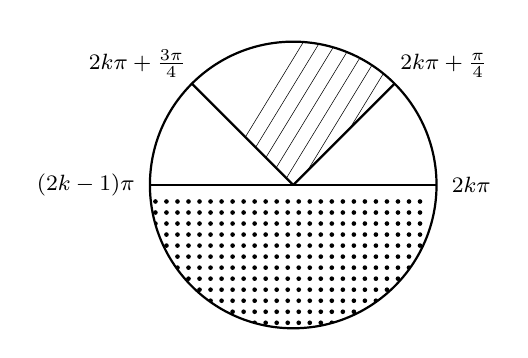
\begin{tikzpicture}[>=latex, scale=1.4]
  % 扇形斜线阴影
  \begin{scope}
    \clip (0,0) -- (45:1.3) arc (45:135:1.3) -- cycle;
    \foreach \x in {-1.8,-1.65,...,1.8} {
      \draw[very thin] (\x,-1.8) -- (\x+2.2,1.8);
    }
  \end{scope}
  % 下半圆点阵阴影
  \begin{scope}
    \clip (-1.3,0) arc (180:360:1.3) -- cycle;
    \foreach \x in {-1.25,-1.15,...,1.25} {
      \foreach \y in {-1.25,-1.15,...,-0.05} {
        \fill (\x,\y) circle (0.6pt);
      }
    }
  \end{scope}
  % 轮廓与分割线
  \draw[thick] (0,0) circle (1.3);
  \draw[thick] (-1.3,0) -- (1.3,0);
  \draw[thick] (0,0) -- (45:1.3);
  \draw[thick] (0,0) -- (135:1.3);
  % 标注
  \node[left=2pt] at (-1.3,0) {\footnotesize $(2k-1)\pi$};
  \node[right=2pt] at (1.3,0) {\footnotesize $2k\pi$};
  \node[above left] at (135:1.25) {\footnotesize $2k\pi+\frac{3\pi}{4}$};
  \node[above right] at (45:1.25) {\footnotesize $2k\pi+\frac{\pi}{4}$};
\end{tikzpicture}
\caption{}\label{fig:1.1.5}
\end{figure}

显然 $n_1<n_2<\cdots$ 且 $n_1'<n_2'<\cdots$. 对于子列 $\{a_{n_k}\}$, 有
\[
  a_{n_k} = \sin n_k > \sin\frac{\pi}{4} = \frac{\sqrt{2}}{2};
\]
而对于子列 $\{a_{n_k'}\}$, 有
\[
  a_{n_k'} = \sin n_k' < 0.
\]
故若极限存在为 $a$, 则必然有 $a\geqslant\frac{\sqrt{2}}{2}$ 且 $a\leqslant 0$, 矛盾! 故数列 $\{\sin n\}$ 无极限.
\end{proof}

\begin{theorem}[保号性与保序性]\label{thm:1.1.6}
设 $\lim_{n\to+\infty} a_n = a > b$ (或 $<b$), 则 $\exists N_0 \in \mathbb{N}$, 当 $n>N_0$ 时有 $a_n > b$ (或 $a_n < b$).
\end{theorem}
\begin{proof}
取 $\varepsilon = a-b > 0$. 由极限定义, $\exists N_0\in\mathbb{N}$, 当 $n>N_0$ 时, 有
\[
  |a_n-a| < \varepsilon \implies a_n > a-\varepsilon = a-(a-b) = b.
\]
同理可证 $a<b$ 的情形.
\end{proof}

\begin{example}\label{ex:1.1.14}
设 $\lim_{n\to+\infty}a_n=0$ (极限为 0 的变量称为无穷小量), 且数列 $\{b_n\}$ 有界 (即 $\exists M>0$ 使 $|b_n|\leqslant M$), 则
\[
  \lim_{n\to+\infty}a_n b_n = 0.
\]
即无穷小量与有界变量之积仍为无穷小量.
\end{example}
\begin{proof}
$\forall\varepsilon>0$, 因 $\lim_{n\to+\infty}a_n=0$, 故 $\exists N\in\mathbb{N}$, 当 $n>N$ 时, 有 $|a_n-0|<\frac{\varepsilon}{M+1}$. 于是
\[
  |a_{n}b_{n}-0|=|a_{n}b_{n}|\leqslant M|a_{n}| \leqslant M\cdot\frac{\varepsilon}{M+1}<\varepsilon,
\]
所以 $\lim_{n\to+\infty}a_n b_n = 0$.
\end{proof}

\begin{example}[Ces\`aro 算术平均]\label{ex:1.1.15}
设 $\lim_{n\to+\infty}a_n=a$ (实数, $+\infty, -\infty$), 则
\[
  \lim_{n\to+\infty}\frac{a_1+a_2+\cdots+a_n}{n}=a.
\]
但反之不真.
\end{example}
\begin{proof}
反之不真显见: 取 $a_n=(-1)^{n-1}$, 则 $\{a_n\}$ 发散, 但 $\frac{a_1+\cdots+a_n}{n}\to 0$.

现在证明正向结论:
当 $a\in\mathbb{R}$ 时, 设 $a_n = a+\alpha_n$, 其中 $\lim_{n\to+\infty}\alpha_n=0$. 则
\[
  \frac{a_1+\cdots+a_n}{n} = a + \frac{\alpha_1+\cdots+\alpha_n}{n}.
\]
$\forall\varepsilon>0$, $\exists N_1\in\mathbb{N}$, 当 $n>N_1$ 时, $|\alpha_n|<\frac{\varepsilon}{2}$. 取定 $N_1$ 后, $\sum_{k=1}^{N_1}|\alpha_k|$ 为常数, 故 $\exists N_2>N_1$, 当 $n>N_2$ 时, $\frac{\sum_{k=1}^{N_1}|\alpha_k|}{n}<\frac{\varepsilon}{2}$. 于是当 $n>N_2$ 时,
\[
  \left|\frac{\alpha_1+\cdots+\alpha_n}{n}\right| \leqslant \frac{\sum_{k=1}^{N_1}|\alpha_k|}{n} + \frac{\sum_{k=N_1+1}^n|\alpha_k|}{n} < \frac{\varepsilon}{2} + \frac{(n-N_1)\frac{\varepsilon}{2}}{n} < \varepsilon.
\]
故 $\lim_{n\to+\infty}\frac{a_1+\cdots+a_n}{n}=a$.

当 $a=+\infty$ 时, $\forall A>0$, $\exists N_1\in\mathbb{N}$, 当 $n>N_1$ 时, $a_n > 2A+2$. 固定 $N_1$, 因 $\lim_{n\to+\infty}\frac{n-N_1}{n}=1>\frac{1}{2}$ 且 $\lim_{n\to+\infty}\frac{a_1+\cdots+a_{N_1}}{n}=0>-1$, 故 $\exists N_2>N_1$, 当 $n>N_2$ 时, 有
\[
  \frac{a_1+\cdots+a_n}{n} = \frac{a_1+\cdots+a_{N_1}}{n} + \frac{a_{N_1+1}+\cdots+a_n}{n} > -1 + \frac{n-N_1}{n}(2A+2) > -1 + \frac{1}{2}(2A+2) = A.
\]
故 $\lim_{n\to+\infty}\frac{a_1+\cdots+a_n}{n}=+\infty$.

$a=-\infty$ 的情形完全类似可证.
\end{proof}

\begin{example}\label{ex:1.1.16}
数列 $\{a_{n}\}$ 无上界 $\iff \{a_{n}\}$ 必有子列 $\{a_{n_{k}}\}$ 使得 $\lim_{k\to+\infty}a_{n_k}=+\infty$.
\end{example}
\begin{proof}
\textbf{充分性:}\quad 若有子列 $a_{n_k}\to+\infty$, 则对任意 $M>0$, 存在 $K$ 使得当 $k>K$ 时 $a_{n_k}>M$, 故原数列无上界.

\textbf{必要性:}\quad 设 $\{a_n\}$ 无上界. 取 $k=1$, $\exists n_1\in\mathbb{N}$ 使 $a_{n_1}>1$.
假设已选出 $n_1<n_2<\cdots<n_{k-1}$ 满足 $a_{n_j}>j\ (j=1,\cdots,k-1)$. 令
\[
  M_k = \max\{k, a_1, a_2, \cdots, a_{n_{k-1}}\}.
\]
因为 $\{a_n\}$ 无上界, 故必存在 $n_k$ 使得 $a_{n_k}>M_k$. 显然 $a_{n_k}>k$, 且由 $a_{n_k}>M_k \geqslant a_i\ (1\leqslant i\leqslant n_{k-1})$ 可知 $n_k > n_{k-1}$.
以此归纳可得子列 $\{a_{n_k}\}$, 满足 $n_1<n_2<\cdots$ 且 $a_{n_k}>k$. 故 $\lim_{k\to+\infty}a_{n_k}=+\infty$.
\end{proof}

\begin{exblock}{练习题 1.1}
\item 用数列极限定义证明:
\begin{enumerate}
  \item $\lim_{n \to +\infty} 0.\underbrace{99 \cdots 9}_n = 1$;
  \item $\lim_{n \to +\infty} \frac{3n + 4}{7n - 3} = \frac{3}{7}$;
  \item $\lim_{n \to +\infty} \frac{5n + 6}{n^2 - n - 1000} = 0$;
  \item $\lim_{n \to +\infty} \frac{8}{2^n + 5} = 0$;
  \item $\lim_{n \to +\infty} \frac{\sin n!}{n^{1/2}} = 0$;
  \item $\lim_{n \to +\infty} (\sqrt{n + 2} - \sqrt{n - 2}) = 0$;
  \item $\lim_{n \to +\infty} (\sqrt[3]{n+2} - \sqrt[3]{n-2}) = 0$;
  \item $\lim_{n \to +\infty} \frac{n^{3/2} \arctan n}{1 + n^2} = 0$;
  \item $\lim_{n \to +\infty} a_n = 1$, 其中 $a_n = \begin{cases} \frac{n-1}{n}, & n \text{ 为偶数}, \\ \frac{\sqrt{n^2 + n}}{n}, & n \text{ 为奇数}; \end{cases}$
  \item $\lim_{n \to +\infty} (n^3 - 4n - 5) = +\infty$.
\end{enumerate}

\item 设 $\lim_{n\to+\infty}a_n=a$. 证明: $\forall k\in\mathbb{N}$, 有 $\lim_{n\to+\infty}a_{n+k}=a$.

\item 设 $\lim_{n\to+\infty}a_n=a$. 证明: $\lim_{n\to+\infty}|a_n|=|a|$. 举例说明, 这个命题的逆命题不真.

\item 设 $x_{n} \leqslant a \leqslant y_{n}, n \in \mathbb{N}$, 且 $\lim_{n\to+\infty}(y_{n}-x_{n})=0$. 证明:
\[
  \lim_{n\to+\infty}x_{n}=\lim_{n\to+\infty}y_{n}=a.
\]

\item 设 $\{a_{n}\}$ 为一个收敛数列. 证明: 数列 $\{a_{n}\}$ 中或者有最大的数, 或者有最小的数. 举出两者都有的例子; 再举出只有一个的例子.

\item 证明下列数列发散:
\begin{enumerate}
  \item $\{n^{(-1)^n}\}$;
  \item $\{\cos n\}$.
\end{enumerate}

\item 证明: 数列 $\{a_{n}\}$ 收敛 $\iff$ 三个数列 $\{a_{3k-2}\}$, $\{a_{3k-1}\}$, $\{a_{3k}\}$ 都收敛且有相同的极限.

\item 设 $\lim_{n\to+\infty}(a_{n}-a_{n-1})=d$. 证明: $\lim_{n\to+\infty}\frac{a_n}{n}=d$.

\item 设 $\lim_{n\to+\infty} a_n = a$. 用 $\varepsilon\text{-}N$ 法, $A\text{-}N$ 法证明:
\[
  \lim_{n\to+\infty}\frac{a_1+2a_2+\cdots+na_n}{n^2}=\frac{a}{2}\quad (a \text{ 为实数}, +\infty, -\infty).
\]
\end{exblock}

\begin{exblock}{思考题 1.1}
\item 设 $\lim_{n\to+\infty}a_n=a$, $|q| < 1$. 用 $\varepsilon\text{-}N$ 法证明:
\[
  \lim_{n\to+\infty}(a_{n}+a_{n-1}q+\cdots+a_{1}q^{n-1})=\frac{a}{1-q}.
\]

\item 设 $\lim_{n\to+\infty}a_n=a$, $\lim_{n\to+\infty}b_n=b$. 用 $\varepsilon\text{-}N$ 法证明:
\[
  \lim_{n\to+\infty}\frac{a_0b_n+a_1b_{n-1}+\cdots+a_{n-1}b_1+a_nb_0}{n}=ab.
\]

\item 设 $\lim_{n\to+\infty}a_n=a, b_n\geqslant 0\ (n\in\mathbb{N}), \lim_{n\to+\infty}(b_1+b_2+\cdots+b_n)=S$. 证明:
\[
  \lim_{n\to+\infty}(a_nb_1+a_{n-1}b_2+\cdots+a_1b_n)=aS.
\]

\item \textbf{(Toeplitz 定理)}\ 设 $n, k \in \mathbb{N}$, $t_{nk} \geqslant 0$ 且 $\sum_{k=1}^{n} t_{nk} = 1$, $\lim_{n \to +\infty} t_{nk} = 0$. 如果 $\lim_{n \to +\infty} a_n = a$, 证明:
\[
  \lim_{n \to +\infty} \sum_{k=1}^{n} t_{nk} a_k = a.
\]
说明例~\ref{ex:1.1.15} 为 Toeplitz 定理的特殊情形.

\item 设 $a, b, c$ 为三个给定的实数, 令 $a_{0} = a, b_{0} = b, c_{0} = c$, 并归纳定义
\[
  \begin{cases}
    a_{n}=\dfrac{b_{n-1}+c_{n-1}}{2},\\[6pt]
    b_{n}=\dfrac{c_{n-1}+a_{n-1}}{2}, & n = 1, 2, \cdots.\\[6pt]
    c_{n}=\dfrac{a_{n-1}+b_{n-1}}{2},
\end{cases}
\]
证明: $\lim_{n\to+\infty}a_n=\lim_{n\to+\infty}b_n=\lim_{n\to+\infty}c_n=\frac{a+b+c}{3}$.

\item 设 $a_{1}, a_{2}$ 为实数, 令
\[
  a_{n}=pa_{n-1}+qa_{n-2},\quad n=3, 4, 5, \cdots,
\]
其中 $p > 0, q > 0, p + q = 1$. 证明: 数列 $\{a_{n}\}$ 收敛, 且 $\lim_{n \to +\infty} a_{n} = \frac{a_{2} + a_{1} q}{1 + q}$.

\item 设数列 $\{a_{n}\}$, $\{b_{n}\}$, $\{c_{n}\}$ 满足 $a_{1} > 0, 4 \leqslant b_{n} \leqslant 5, 4 \leqslant c_{n} \leqslant 5$,
\[
  a_{n}=\frac{\sqrt{b_{n}^{2}+c_{n}^{2}}}{b_{n}+c_{n}}a_{n-1}.
\]
证明: $\lim_{n\to+\infty}a_n = 0$.
\end{exblock}

\section{数列极限的基本性质}\label{sec:1.2}

在定义了数列极限之后，我们会用 $\varepsilon\text{-}N$ 法证明一些数列的极限，但从上节知道，这必须在已知数列有无极限的前提下才能应用，且某些证明还相当复杂，有些甚至还无法用 $\varepsilon\text{-}N$ 法证明。所以，我们必须进一步了解数列极限有哪些性质，还有什么方法可以使用。为此，本节将逐一给出数列极限的唯一性，收敛数列的有界性，极限的四则运算性质，不等式性质以及重要的夹逼定理。

\begin{theorem}[极限的惟一性]\label{thm:1.2.1}
设数列 $\{a_{n}\}$ 有极限（实数，或 $+\infty$，或 $-\infty$），则极限是惟一的。
\end{theorem}

\begin{proof}
\textbf{证法 1} 设 $\lim\limits_{n\to+\infty}a_n=a$ 及 $\lim\limits_{n\to+\infty}a_n=b$，$a,b\in\mathbb{R}$。

（反证）反设 $a \neq b$。令 $\varepsilon_{0} = |a - b| > 0$，根据数列极限的定义~\ref{def:1.1.1}，$\exists N \in \mathbb{N}$，当 $n > N$ 时，
\[
|a_{n}-a|<\frac{\varepsilon_{0}}{2},\quad |a_{n}-b|<\frac{\varepsilon_{0}}{2},
\]
所以，
\[
|a-b| \leqslant |a-a_{n}| + |a_{n}-b| < \frac{\varepsilon_{0}}{2} + \frac{\varepsilon_{0}}{2} = \varepsilon_{0} = |a-b|,
\]
矛盾。

值得注意的是这种证法不能应用到极限为 $+\infty$ 或 $-\infty$ 的情况，因此还必须给出能推广到 $+\infty$ 或 $-\infty$ 的证法，于是有下面证法。

\textbf{证法 2} 设 $\lim\limits_{n\to+\infty}a_n=a$ 及 $\lim\limits_{n\to+\infty}a_n=b$，$a,b\in\mathbb{R}$。

（反证）反设 $a \neq b$，不失一般性，设 $a < b$。令 $\varepsilon_{0} = \frac{b - a}{2} > 0$。由极限定义~\ref{def:1.1.1} 知，$\exists N_{1} \in \mathbb{N}$，当 $n > N_{1}$ 时，$a - \varepsilon_{0} < a_{n} < a + \varepsilon_{0}$；$\exists N_{2} \in \mathbb{N}$，当 $n > N_{2}$ 时，$b - \varepsilon_{0} < a_{n} < b + \varepsilon_{0}$。所以，当 $n > N = \max\{N_{1}, N_{2}\}$ 时，
\[
\frac{a+b}{2} = b - \frac{b-a}{2} = b - \varepsilon_{0} < a + \varepsilon_{0} = a + \frac{b-a}{2} = \frac{a+b}{2},
\]
矛盾。

其他情形类似证明。

\textbf{证法 3}（统一描述）设 $\lim\limits_{n\to+\infty}a_n=a$ 及 $\lim\limits_{n\to+\infty}a_n=b$。

（反证）反设 $a \neq b$，不妨设 $a < b$，则存在 $a$ 的开邻域 $U_a$ 与 $b$ 的开邻域 $U_b$，使得 $U_a \cap U_b = \varnothing$。由极限定义~\ref{def:1.1.1} 知，$\exists N_1 \in \mathbb{N}$，当 $n > N_1$ 时，$a_n \in U_a$；$\exists N_2 \in \mathbb{N}$，当 $n > N_2$ 时，$a_n \in U_b$。所以，当 $n > \max\{N_1, N_2\}$ 时，$a_n \in U_a \cap U_b = \varnothing$，矛盾。
\end{proof}

\begin{definition}\label{def:1.2.1}
如果存在实数 $M>0$，使得对任何自然数 $n$，有 $|a_{n}| \leqslant M$，则称数列 $\{a_{n}\}$ \textbf{有界}。如果存在实数 $B$，使得 $a_{n} \leqslant B$（$\forall n \in \mathbb{N}$），则称数列 $\{a_{n}\}$ \textbf{有上界} $B$。如果存在实数 $A$，使得 $a_{n} \geqslant A$（$\forall n \in \mathbb{N}$），则称数列 $\{a_{n}\}$ \textbf{有下界} $A$。
\end{definition}

显然，$\{a_{n}\}$ 有界的充要条件是 $\{a_{n}\}$ 既有上界又有下界。

\begin{theorem}\label{thm:1.2.2}
数列 $\{a_{n}\}$ 收敛，则 $\{a_{n}\}$ 必有界。反之不真。
\end{theorem}

\begin{proof}
设 $\lim\limits_{n \to \infty} a_n = a \in \mathbb{R}$。取 $\varepsilon_0 = 1$，$\exists N_0 \in \mathbb{N}$，当 $n > N_0$ 时，$|a_n - a| < \varepsilon_0 = 1$，所以，
\[
|a_{n}| = |(a_{n}-a)+a| \leqslant |a_{n}-a| + |a| < 1 + |a|.
\]
于是，$\forall n \in \mathbb{N}$，有
\[
|a_{n}| \leqslant \max\{|a_{1}|, \cdots, |a_{N_{0}}|, |a|+1\} = M,
\]
即数列 $\{a_{n}\}$ 有界。

反之则有反例 $a_{n}=(-1)^{n-1}$，满足 $|a_{n}| \leqslant 1$，有界。但由例 1.1.12 已知，$a_{n}=(-1)^{n-1}$ 时数列发散。
\end{proof}

\begin{theorem}[极限的四则运算]\label{thm:1.2.3}
设 $\{a_{n}\}, \{b_{n}\}$ 都收敛，则 $\{a_{n}\pm b_{n}\}, \{a_{n}b_{n}\}$ 也收敛。又若 $\lim\limits_{n\to+\infty}b_{n}\neq0$，则 $\left\{\frac{a_{n}}{b_{n}}\right\}$ 也收敛。且
\begin{enumerate}
  \item $\lim\limits_{n \to +\infty} (a_n \pm b_n) = \lim\limits_{n \to +\infty} a_n \pm \lim\limits_{n \to +\infty} b_n$；
  \item $\lim\limits_{n\to+\infty} a_n b_n = \lim\limits_{n\to+\infty} a_n \cdot \lim\limits_{n\to+\infty} b_n$，特别有 $\lim\limits_{n\to+\infty} c a_n = c \lim\limits_{n\to+\infty} a_n$；
  \item $\lim\limits_{n \to +\infty} \frac{a_n}{b_n} = \frac{\lim\limits_{n \to +\infty} a_n}{\lim\limits_{n \to +\infty} b_n}\ (\lim\limits_{n \to +\infty} b_n \neq 0)$。
\end{enumerate}
\end{theorem}

\begin{proof}
(1) $\forall \varepsilon > 0$，因 $\lim\limits_{n \to +\infty} a_n = a \in \mathbb{R}$，$\lim\limits_{n \to +\infty} b_n = b \in \mathbb{R}$，所以，$\exists N_1 \in \mathbb{N}$，当 $n > N_1$ 时，$|a_n - a| < \frac{\varepsilon}{2}$；$\exists N_2 \in \mathbb{N}$，当 $n > N_2$ 时，$|b_n - b| < \frac{\varepsilon}{2}$。于是，当 $n > N = \max\{N_1, N_2\}$ 时，
\begin{align*}
|(a_{n}\pm b_{n})-(a\pm b)| &= |(a_{n}-a)\pm(b_{n}-b)| \\
&\leqslant |a_{n}-a| + |b_{n}-b| \\
&< \frac{\varepsilon}{2} + \frac{\varepsilon}{2} = \varepsilon,
\end{align*}
由此就有 $\lim\limits_{n\to+\infty}(a_n\pm b_n) = a\pm b = \lim\limits_{n\to+\infty}a_n \pm \lim\limits_{n\to+\infty}b_n$。

(2) 因为 $\lim\limits_{n \to +\infty} b_n = b \in \mathbb{R}$，由定理~\ref{thm:1.2.2} 可知，$|b_n| < M$（$\forall n \in \mathbb{N}$）。又因 $\lim\limits_{n \to +\infty} a_n = a \in \mathbb{R}$，故 $\forall \varepsilon > 0$，$\exists N \in \mathbb{N}$，当 $n > N$ 时，
\[
|a_{n}-a| < \frac{\varepsilon}{2M},\quad |b_{n}-b| < \frac{\varepsilon}{2(|a|+1)},
\]
及
\begin{align*}
|a_{n}b_{n}-ab| &= |a_{n}b_{n}-ab_{n}+ab_{n}-ab| \leqslant |b_{n}||a_{n}-a| + |a||b_{n}-b| \\
&< M \frac{\varepsilon}{2M} + |a| \frac{\varepsilon}{2(|a|+1)} < \frac{\varepsilon}{2} + \frac{\varepsilon}{2} = \varepsilon.
\end{align*}
这就证明了
\[
\lim_{n\to+\infty}a_nb_n = ab = \lim_{n\to+\infty}a_n \cdot \lim_{n\to+\infty}b_n.
\]

(3) 先证：如果 $\lim\limits_{n\to+\infty}b_n=b\neq0$，则 $\lim\limits_{n\to+\infty}\frac{1}{b_n}=\frac{1}{b}$。事实上，$\forall\varepsilon>0$，$\exists N\in\mathbb{N}$，当 $n>N$ 时，
\[
|b_{n}-b| < \min\left\{\frac{|b|}{2}, \frac{b^{2}}{2}\varepsilon\right\}.
\]
则当 $n > N$ 时，有
\[
|b_{n}| = |(b_{n}-b)+b| \geqslant |b| - |b_{n}-b| > |b| - \frac{|b|}{2} = \frac{|b|}{2},
\]
\[
\left|\frac{1}{b_{n}}-\frac{1}{b}\right| = \frac{|b_{n}-b|}{|b_{n}||b|} < \frac{|b_{n}-b|}{\frac{|b|}{2}|b|} < \frac{2}{b^{2}} \cdot \frac{b^{2}}{2}\varepsilon = \varepsilon.
\]
这就证明了
\[
\lim_{n\to+\infty}\frac{1}{b_{n}} = \frac{1}{b}.
\]
由此得到
\[
\lim_{n\to+\infty}\frac{a_{n}}{b_{n}} = \lim_{n\to+\infty}a_{n} \cdot \frac{1}{b_{n}} = a \cdot \frac{1}{b} = \frac{a}{b} = \frac{\lim\limits_{n\to+\infty}a_{n}}{\lim\limits_{n\to+\infty}b_{n}}.
\]
\end{proof}

\begin{theorem}\label{thm:1.2.4}
设 $\lim\limits_{n\to+\infty}a_n=a$，$\lim\limits_{n\to+\infty}b_n=b$，$a<b$。则存在自然数 $N_0$，当 $n>N_0$ 时，有 $a_n<b_n$。
\end{theorem}

\begin{proof}
\textbf{证法 1} 当 $a, b \in \mathbb{R}$ 时，令 $\varepsilon_{0} = \frac{b - a}{2} > 0$。因 $\lim\limits_{n \to +\infty} a_{n} = a$，$\lim\limits_{n \to +\infty} b_{n} = b$，则存在自然数 $N_{0}$，当 $n > N_{0}$ 时，有
\[
\frac{3a-b}{2} = a - \frac{b-a}{2} < a_{n} < a + \frac{b-a}{2} = \frac{a+b}{2},
\]
\[
\frac{a+b}{2} = b - \frac{b-a}{2} < b_{n} < b + \frac{b-a}{2} = \frac{3b-a}{2},
\]
所以，
\[
a_{n} < \frac{a+b}{2} < b_{n}.
\]
其他情形类似证明。

\textbf{证法 2}（统一描述）因为 $\lim\limits_{n\to+\infty}a_n=a < b = \lim\limits_{n\to+\infty}b_n$，所以存在 $a$ 的开邻域 $U_a$，$b$ 的开邻域 $U_b$，使得 $U_a \cap U_b = \varnothing$。并且 $\exists N_0 \in \mathbb{N}$，当 $n > N_0$ 时，$a_n \in U_a$，$b_n \in U_b$，所以 $a_n < b_n$。
\end{proof}

\begin{theorem}\label{thm:1.2.5}
设 $a_{n} \leqslant b_{n}$（$n = N_{0}, N_{0} + 1, \cdots$），$\lim\limits_{n \to \infty} a_{n} = a$，$\lim\limits_{n \to \infty} b_{n} = b$，则 $a \leqslant b$。
\end{theorem}

\begin{proof}
（反证）反设 $a > b$，根据定理~\ref{thm:1.2.4} 知，$\exists N \in \mathbb{N}, N > N_0$，当 $n > N$ 时，有 $a_n > b_n$，这与 $a_n \leqslant b_n$（$n \geqslant N > N_0$）矛盾。
\end{proof}

\begin{theorem}[夹逼定理]\label{thm:1.2.6}
设数列 $\{a_{n}\}$，$\{b_{n}\}$，$\{c_{n}\}$ 满足 $a_{n} \leqslant b_{n} \leqslant c_{n}$（$n > N_{0}$），$\lim\limits_{n \to +\infty} a_{n} = a = \lim\limits_{n \to +\infty} c_{n}$，$a$ 为实数、$+\infty$ 或 $-\infty$，则 $\lim\limits_{n \to +\infty} b_{n} = a$。
\end{theorem}

\begin{proof}
\textbf{证法 1} 当 $a$ 为实数时，$\forall \varepsilon > 0$，因为 $\lim\limits_{n \to +\infty} a_n = a = \lim\limits_{n \to +\infty} c_n$，所以，$\exists N \in \mathbb{N}, N > N_0$，当 $n > N$ 时，
\[
a-\varepsilon < a_{n} < a+\varepsilon,
\]
\[
a-\varepsilon < c_{n} < a+\varepsilon.
\]
再由已知可得
\[
a-\varepsilon < a_{n} \leqslant b_{n} \leqslant c_{n} < a+\varepsilon,
\]
这就证明了 $\lim\limits_{n\to+\infty}b_{n}=a$。

其他情形类似证明。

\textbf{证法 2}（统一描述）对 $a$ 的任何开邻域（区间）$U$，因为 $\lim\limits_{n\to+\infty}a_n = a = \lim\limits_{n\to+\infty}c_n$，所以，$\exists N\in\mathbb{N}$，当 $n>N$ 时，有 $a_n\in U, c_n\in U$。又由已知 $b_n\in[a_n,c_n]\subset U$，这就证明了 $\lim\limits_{n\to+\infty}b_n=a$。
\end{proof}

\begin{remark}\label{rem:1.2.1}
夹逼定理对 $a=\infty$ 不成立。

反例：$a_{n}=-n, b_{n}=0$ 或 $(-1)^{n-1}, c_{n}=n$，则 $\lim\limits_{n\to+\infty}a_{n}=\infty=\lim\limits_{n\to+\infty}c_{n}$，但 $\lim\limits_{n\to+\infty}b_{n}\neq\infty$。
\end{remark}

\begin{theorem}\label{thm:1.2.7}
\begin{enumerate}
  \item 设 $a_{n} \geqslant b_{n}$（$n \geqslant N_{0}$），$\lim\limits_{n \to +\infty} b_{n} = +\infty$，则 $\lim\limits_{n \to \infty} a_{n} = +\infty$；
  \item 设 $\lim\limits_{n\to+\infty}a_n=+\infty$，$\lim\limits_{n\to+\infty}b_n=+\infty$，则 $\lim\limits_{n\to+\infty}(a_n+b_n)=+\infty$；
  \item $\lim\limits_{n\to+\infty}a_n=a\in\mathbb{R}$，$\lim\limits_{n\to+\infty}b_n=\pm\infty$，则 $\lim\limits_{n\to+\infty}(a_n+b_n)=\pm\infty$；
  \item $\lim\limits_{n\to+\infty}a_n=a>0$，$\lim\limits_{n\to+\infty}b_n=\pm\infty$，则 $\lim\limits_{n\to+\infty}a_n b_n=\pm\infty$；
  \item $\lim\limits_{n\to+\infty}a_n=a<0$，$\lim\limits_{n\to+\infty}b_n=\pm\infty$，则 $\lim\limits_{n\to+\infty}a_n b_n=\mp\infty$；
  \item $\lim\limits_{n \to +\infty} a_n = +\infty \iff \lim\limits_{n \to +\infty} (-a_n) = -\infty$；
  \item $\lim\limits_{n \to +\infty} a_n = \infty \iff \lim\limits_{n \to +\infty} \frac{1}{a_n} = 0$。
\end{enumerate}
\end{theorem}

\begin{proof}
只证明 (4)，(7)，其他读者自证。

(4) 因为 $\lim\limits_{n \to +\infty} a_n = a > 0$，由定理 1.1.6 可知，$\exists N_1 \in \mathbb{N}$，当 $n > N_1$ 时，有 $a_n > \frac{a}{2}$。又因 $\lim\limits_{n \to +\infty} b_n = +\infty$，故 $\forall A > 0$，$\exists N_2 \in \mathbb{N}$，当 $n > N_2$ 时，$b_n > \frac{2A}{a}$。于是，当 $n > N = \max\{N_1, N_2\}$ 时，
\[
a_{n}b_{n} > \frac{a}{2} \cdot \frac{2A}{a} = A,
\]
这就证明了 $\lim\limits_{n\to+\infty}a_nb_n=+\infty$。

(7) ($\Rightarrow$) $\forall \varepsilon > 0$，取 $A = \frac{1}{\varepsilon} > 0$，因 $\lim\limits_{n \to +\infty} a_n = \infty$，故 $\exists N \in \mathbb{N}$，当 $n > N$ 时，$|a_n| > A = \frac{1}{\varepsilon}$，即
\[
\left|\frac{1}{a_{n}}-0\right| = \frac{1}{|a_{n}|} < \varepsilon,
\]
这就证明了 $\lim\limits_{n\to+\infty}\frac{1}{a_n}=0$。

($\Leftarrow$) $\forall A>0$，取 $\varepsilon=\frac{1}{A}>0$，因 $\lim\limits_{n\to+\infty}\frac{1}{a_n}=0$，故 $\exists N\in\mathbb{N}$，当 $n>N$ 时，有
\[
\frac{1}{|a_{n}|} = \left|\frac{1}{a_{n}}-0\right| < \varepsilon = \frac{1}{A},\quad |a_{n}| > A,
\]
这就证明了 $\lim\limits_{n\to+\infty}a_n=\infty$。
\end{proof}

应用这些性质和定理，求下面数列的极限就比较容易。

\begin{example}\label{ex:1.2.1}
求
\begin{enumerate}
  \item $\lim\limits_{n \to +\infty} \frac{n^3 - n + 1}{4n^3 + n^2 - 1}$；
  \item $\lim\limits_{n \to +\infty} \frac{2n^2 + n + 1}{2n - 1}$。
\end{enumerate}
\end{example}

\begin{solution}
(1) 
\begin{align*}
\lim_{n\to+\infty}\frac{3n^{3}-n+1}{4n^{3}+n^{2}-1} &= \lim_{n\to+\infty}\frac{3-\frac{1}{n^{2}}+\frac{1}{n^{3}}}{4+\frac{1}{n}-\frac{1}{n^{3}}} \\
&\xlongequal{\text{定理~\ref{thm:1.2.3}}} \frac{3-0+0}{4+0-0} = \frac{3}{4}.
\end{align*}
\footnote{原书例 1.2.1 题干中分子印为 $n^3-n+1$，解中为 $3n^3-n+1$。}也可以用 $\varepsilon\text{-}N$ 法证其极限为 $\frac{3}{4}$。

(2)
\begin{align*}
\lim_{n\to+\infty}\frac{2n^{2}+n+1}{2n-1} &= \lim_{n\to+\infty}\frac{n^{2}(2+\frac{1}{n}+\frac{1}{n^{2}})}{n(2-\frac{1}{n})} \\
&= \lim_{n\to+\infty}n \cdot \frac{2+\frac{1}{n}+\frac{1}{n^{2}}}{2-\frac{1}{n}} \\
&\xlongequal{\text{定理~\ref{thm:1.2.7}(4)}} +\infty.
\end{align*}
\end{solution}

更一般地有以下例子。

\begin{example}\label{ex:1.2.2}
设 $a_{0} \neq 0, b_{0} \neq 0$，则
\[
\lim_{n\to+\infty}\frac{a_0n^k+a_1n^{k-1}+\cdots+a_{k-1}n+a_k}{b_0n^l+b_1n^{l-1}+\cdots+b_{l-1}n+b_l} = \begin{cases}
\dfrac{a_0}{b_0}, & k=l, \\
0, & k<l, \\
+\infty, & k>l,\ \dfrac{a_0}{b_0}>0, \\
-\infty, & k>l,\ \dfrac{a_0}{b_0}<0.
\end{cases}
\]
\end{example}

\begin{proof}
\begin{align*}
&\lim_{n\to+\infty}\frac{a_0n^k+a_1n^{k-1}+\cdots+a_{k-1}n+a_k}{b_0n^l+b_1n^{l-1}+\cdots+b_{l-1}n+b_l} \\
&= \lim_{n\to+\infty}n^{k-l}\frac{a_0+\frac{a_1}{n}+\cdots+\frac{a_{k-1}}{n^{k-1}}+\frac{a_k}{n^k}}{b_0+\frac{b_1}{n}+\cdots+\frac{b_{l-1}}{n^{l-1}}+\frac{b_l}{n^l}} \\
&= \begin{cases}
1 \cdot \dfrac{a_0+0+\cdots+0}{b_0+0+\cdots+0}, & k=l, \\
0 \cdot \dfrac{a_0+0+\cdots+0}{b_0+0+\cdots+0}, & k<l, \\
+\infty, & k>l,\ \dfrac{a_0}{b_0}>0, \\
-\infty, & k>l,\ \dfrac{a_0}{b_0}<0
\end{cases}
= \begin{cases}
\dfrac{a_0}{b_0}, & k=l, \\
0, & k<l, \\
+\infty, & k>l,\ \dfrac{a_0}{b_0}>0, \\
-\infty, & k>l,\ \dfrac{a_0}{b_0}<0.
\end{cases}
\end{align*}
\end{proof}

\begin{example}\label{ex:1.2.3}
求 $\sum\limits_{n=0}^{\infty} q^{n} = \lim\limits_{n \to +\infty} (1 + q + q^{2} + \cdots + q^{n-1})$。
\end{example}

\begin{solution}
当 $q \neq \pm 1$ 时，
\begin{align*}
\sum_{n=0}^{\infty}q^{n} &= \lim_{n\to+\infty}(1+q+q^{2}+\cdots+q^{n-1}) = \lim_{n\to+\infty}\frac{1-q^{n}}{1-q} \\
&= \begin{cases}
\dfrac{1-0}{1-q} = \dfrac{1}{1-q}, & \text{当 } |q|<1, \\
+\infty, & \text{当 } q>1, \\
\infty, & \text{当 } q<-1.
\end{cases}
\end{align*}

当 $q=1$ 时，$\lim\limits_{n\to+\infty}(1+q+q^{2}+\cdots+q^{n-1}) = \lim\limits_{n\to+\infty}n = +\infty$。

当 $q = -1$ 时，因为
\[
S_{n} = 1+q+q^{2}+\cdots+q^{n-1} = \begin{cases}
0, & n \text{ 为偶数}, \\
1, & n \text{ 为奇数},
\end{cases}
\]
所以，$\lim\limits_{n\to+\infty}(1+q+q^2+\cdots+q^{n-1})$ 不存在。

综上所述得到
\[
\lim_{n\to+\infty}(1+q+q^{2}+\cdots+q^{n-1}) = \begin{cases}
\dfrac{1}{1-q}, & |q|<1, \\
+\infty, & q\geqslant 1, \\
\infty, & q<-1, \\
\text{不存在}, & q=-1.
\end{cases}
\]
\end{solution}

\begin{example}\label{ex:1.2.4}
计算由曲线 $y=x^{2}$，$y=0$，$x=1$ 所围曲边三角形的面积 $S$。
\end{example}

\begin{solution}
为求出图~\ref{fig:1.2.1} 中曲边三角形的面积，我们采用“以直代曲”的方法。将 $[0,1]$ 区间 $n$ 等分，分点依次为 $0=x_{0}<x_{1}<\cdots<x_{n}=1$，易知 $x_{i}=\frac{i}{n}$，$x_{i}-x_{i-1}=\frac{1}{n}$（$i=1,2,\cdots,n$）。由直线 $x=x_{i}$（$i=0,1,\cdots,n$）将曲边三角形分成 $n$ 条，每一条用直线 $x = x_{i-1}$，$x = x_i$，$y = 0$ 和 $y = y_i = x_{i-1}^2 = \left( \frac{i-1}{n} \right)^2$（$i=1,\cdots,n$）围成的矩形来近似代替。容易看出，$n$ 越大，小矩形面积之和就越逼近曲边三角形的面积，因此我们就用矩形面积之和当 $n \to +\infty$ 时的极限作为该曲边三角形的面积。第 $i$ 条小矩形的面积为 $\Delta S_i = y_i (x_i - x_{i-1}) = \left( \frac{i-1}{n} \right)^2 \frac{1}{n}$（$i=1,2,\cdots,n$），于是曲边三角形的面积为

\begin{figure}[htbp]
\centering
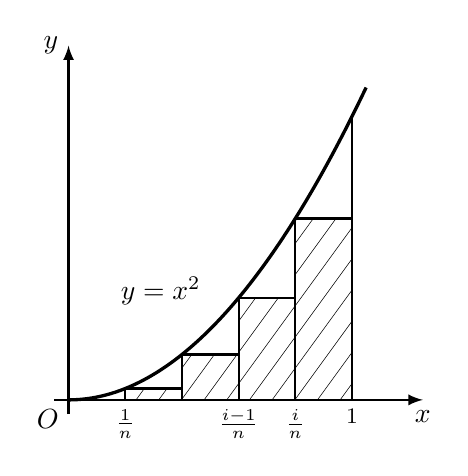
\begin{tikzpicture}[>=latex, scale=3.6]
  % 坐标轴
  \draw[->, thick] (-0.05, 0) -- (1.25, 0) node[below] {$x$};
  \draw[->, thick] (0, -0.05) -- (0, 1.25) node[left] {$y$};
  \node[below left] at (0, 0) {$O$};

  % 抛物线 y = x^2
  \draw[very thick, domain=0:1.05, smooth, samples=50] plot (\x, {\x*\x});
  \node[above left] at (0.5, 0.3) {$y=x^2$};

  % 阶梯小矩形 (示意以直代曲)
  % 矩形 i: [ (i-1)/n, i/n ], 高度 ((i-1)/n)^2
  \foreach \k/\h in {0.2/0.04, 0.4/0.16, 0.6/0.36, 0.8/0.64} {
    \draw[thick] (\k, 0) -- (\k, \h) -- (\k+0.2, \h) -- (\k+0.2, 0);
    \begin{scope}
      \clip (\k, 0) rectangle (\k+0.2, \h);
      \foreach \s in {-0.3, -0.22, ..., 1.2} {
        \draw[very thin] (\s, -0.3) -- (\s+0.8, 0.8);
      }
    \end{scope}
  }

  % x = 1 处的竖线到抛物线 (1,1)
  \draw[thick] (1, 0) -- (1, 1);

  % 轴上刻度与标注
  \node[below] at (0.2, 0) {\footnotesize $\frac{1}{n}$};
  \node[below] at (0.6, 0) {\footnotesize $\frac{i-1}{n}$};
  \node[below] at (0.8, 0) {\footnotesize $\frac{i}{n}$};
  \node[below] at (1.0, 0) {\footnotesize $1$};

  \draw (0.2, 0) -- (0.2, 0.02);
  \draw (0.4, 0) -- (0.4, 0.02);
  \draw (0.6, 0) -- (0.6, 0.02);
  \draw (0.8, 0) -- (0.8, 0.02);
  \draw (1.0, 0) -- (1.0, 0.02);
\end{tikzpicture}
\caption{}\label{fig:1.2.1}
\end{figure}

\begin{align*}
S &= \lim_{n\to+\infty}\left(\Delta S_{1}+\Delta S_{2}+\cdots+\Delta S_{n}\right) \\
&= \lim_{n\to+\infty}\frac{1}{n}\left[\left(\frac{1}{n}\right)^{2}+\left(\frac{2}{n}\right)^{2}+\cdots+\left(\frac{n-1}{n}\right)^{2}\right] \\
&= \lim_{n\to+\infty}\frac{1^{2}+2^{2}+\cdots+(n-1)^{2}}{n^{3}} = \lim_{n\to+\infty}\frac{(n-1)n(2n-1)}{6n^{3}} \\
&= \frac{1}{6}\lim_{n\to+\infty}\left(1-\frac{1}{n}\right)\left(2-\frac{1}{n}\right) = \frac{1}{3}.
\end{align*}
\end{solution}

\begin{example}\label{ex:1.2.5}
求下列极限：
\begin{enumerate}
  \item $\lim\limits_{n \to +\infty} (\sqrt{n+3} - \sqrt{n+1})$；
  \item $\lim\limits_{n \to +\infty} (\sqrt[3]{n+3} - \sqrt[3]{n+1})$；
  \item $\lim\limits_{n \to +\infty}\sqrt[n]{\lg n}$；
  \item $\lim\limits_{n\to+\infty}\sqrt[n]{a_1^n+a_2^n+\cdots+a_m^n}$（$a_i\geqslant0, i=1,2,\cdots,m$）；
  \item $\lim\limits_{n \to +\infty} [(n+1)^k - n^k]$（$0 < k < 1$）；
  \item $\lim\limits_{n \to +\infty} \left( \frac{1}{\sqrt{n^2 + 1}} + \cdots + \frac{1}{\sqrt{n^2 + n}} \right)$；
  \item $\lim\limits_{n \to +\infty} \frac{n^k}{a^n}$（$a > 1$）。
\end{enumerate}
\end{example}

\begin{solution}
(1) 因为
\[
0 < \sqrt{n+3}-\sqrt{n+1} = \frac{2}{\sqrt{n+3}+\sqrt{n+1}} < \frac{1}{\sqrt{n}} \to 0\quad (n\to+\infty),
\]
所以，由夹逼定理（或 $\varepsilon\text{-}N$ 法）知
\[
\lim_{n\to+\infty}(\sqrt{n+3}-\sqrt{n+1}) = 0.
\]

(2) 因为
\begin{align*}
0 &< \sqrt[3]{n+3}-\sqrt[3]{n+1} = \frac{2}{(\sqrt[3]{n+3})^2+\sqrt[3]{n+3}\sqrt[3]{n+1}+(\sqrt[3]{n+1})^2} \\
&< \frac{2}{3(\sqrt[3]{n})^2} = \frac{2}{3n^{\frac{2}{3}}} \to 0\quad (n\to+\infty),
\end{align*}
所以，由夹逼定理（或 $\varepsilon\text{-}N$ 法）知，
\[
\lim_{n\to+\infty}(\sqrt[3]{n+3}-\sqrt[3]{n+1}) = 0.
\]

(3) 因为
\[
10^{n} = (1+9)^{n} > 9n > n \iff 10 > n^{\frac{1}{n}} \iff 1 > \lg n^{\frac{1}{n}} = \frac{\lg n}{n} \iff \lg n < n,
\]
所以，
\[
\sqrt[n]{\lg 2} \leqslant \sqrt[n]{\lg n} < \sqrt[n]{n}.
\]
再由 $\lim\limits_{n\to+\infty}\sqrt[n]{\lg2} = 1 = \lim\limits_{n\to+\infty}\sqrt[n]{n}$ 及夹逼定理就得到
\[
\lim_{n\to+\infty}\sqrt[n]{\lg n} = 1.
\]
\textbf{注意}：虽然数列 $\{\sqrt[n]{a}\}$ 与数列 $\{\sqrt[n]{n}\}$ 的极限相同，但二者之间留有很大的空隙，这使得应用夹逼定理有极大的施展余地。

(4) 由下列不等式
\begin{align*}
\max\{a_{1},a_{2},\cdots,a_{m}\} &= \sqrt[n]{(\max\{a_{1},a_{2},\cdots,a_{m}\})^{n}} \leqslant \sqrt[n]{a_{1}^{n}+a_{2}^{n}+\cdots+a_{m}^{n}} \\
&\leqslant \sqrt[n]{n \cdot (\max\{a_{1},a_{2},\cdots,a_{m}\})^{n}} \\
&= \sqrt[n]{n}\max\{a_{1},a_{2},\cdots,a_{m}\} \to 1 \cdot \max\{a_{1},a_{2},\cdots,a_{m}\} \\
&= \max\{a_{1},a_{2},\cdots,a_{m}\}\quad (n\to+\infty)
\end{align*}
和夹逼定理知，
\[
\lim_{n\to+\infty}\sqrt[n]{a_{1}^{n}+a_{2}^{n}+\cdots+a_{m}^{n}} = \max\{a_{1},a_{2},\cdots,a_{m}\}.
\]

(5) 因为有不等式
\begin{align*}
0 < (n+1)^{k}-n^{k} &= n^{k}\left[\left(1+\frac{1}{n}\right)^{k}-1\right] < n^{k}\left[\left(1+\frac{1}{n}\right)-1\right] \\
&= \frac{1}{n^{1-k}} \to 0\quad (n\to+\infty),
\end{align*}
所以，由夹逼定理（或 $\varepsilon\text{-}N$ 法）得
\[
\lim_{n\to+\infty}[(n+1)^k-n^k] = 0.
\]

(6) 由不等式
\[
\frac{1}{1+\frac{1}{n}} < \frac{1}{\sqrt{1+\frac{1}{n}}} = \frac{n}{\sqrt{n^{2}+n}} \leqslant \frac{1}{\sqrt{n^{2}+1}}+\cdots+\frac{1}{\sqrt{n^{2}+n}} \leqslant \frac{n}{\sqrt{n^{2}+1}} < 1,
\]
$\lim\limits_{n\to+\infty}\frac{1}{1+\frac{1}{n}} = 1 = \lim\limits_{n\to+\infty}1$，以及夹逼定理立即可得
\[
\lim_{n\to+\infty}\left(\frac{1}{\sqrt{n^2+1}}+\cdots+\frac{1}{\sqrt{n^2+n}}\right) = 1.
\]

(7) 因 $a>1$，故 $\alpha = a-1 > 0$。从而
\[
0 < \frac{n^{k}}{a^{n}} = \frac{n^{k}}{(1+\alpha)^{n}} \leqslant \frac{n^{[|k|]+1}}{\mathrm{C}_{n}^{[|k|]+2}\alpha^{[|k|]+2}} \to 0\quad (n\to+\infty),
\]
再根据夹逼定理，就得 $\lim\limits_{n\to+\infty}\frac{n^k}{a^n} = 0$。
\end{solution}

\begin{example}\label{ex:1.2.6}
\begin{enumerate}
  \item 设 $a_{n} \geqslant 0$（$n \in \mathbb{N}$），$\lim\limits_{n \to +\infty} a_{n} = 0$，则 $\lim\limits_{n \to +\infty} \sqrt[n]{a_1 a_2 \cdots a_n} = 0$；
  \item 设 $a_n > 0$（$n \in \mathbb{N}$），$\lim\limits_{n \to +\infty} a_n = a > 0$，则 $\lim\limits_{n \to +\infty} \sqrt[n]{a_1 a_2 \cdots a_n} = a$。
\end{enumerate}
\end{example}

\begin{proof}
(1) 由 $0 \leqslant \sqrt[n]{a_1 a_2 \cdots a_n} \leqslant \frac{a_1 + a_2 + \cdots + a_n}{n} \to 0$（$n \to +\infty$），及夹逼定理，立即可得 $\lim\limits_{n \to +\infty} \sqrt[n]{a_1 a_2 \cdots a_n} = 0$。

(2) 当 $a>0, a_{n}>0$（$n\in\mathbb{N}$）时，有
\[
\frac{1}{\left(\frac{1}{a_{1}}+\frac{1}{a_{2}}+\cdots+\frac{1}{a_{n}}\right)/n} = \frac{n}{\frac{1}{a_{1}}+\frac{1}{a_{2}}+\cdots+\frac{1}{a_{n}}} \leqslant \sqrt[n]{a_{1}a_{2}\cdots a_{n}} \leqslant \frac{a_{1}+a_{2}+\cdots+a_{n}}{n},
\]
再由 $\lim\limits_{n\to+\infty}\frac{1}{\left(\frac{1}{a_1}+\frac{1}{a_2}+\cdots+\frac{1}{a_n}\right)/n} = \frac{1}{\frac{1}{a}} = a = \lim\limits_{n\to+\infty}\frac{a_1+a_2+\cdots+a_n}{n}$ 和夹逼定理，可得
\[
\lim_{n\to+\infty}\sqrt[n]{a_{1}a_{2}\cdots a_{n}} = a.
\]
\end{proof}

\begin{example}\label{ex:1.2.7}
设 $\lim\limits_{n\to+\infty}\sqrt[n]{|a_n|}=r>1$，则 $\lim\limits_{n\to+\infty}a_n=\infty$。
\end{example}

\begin{proof}
\textbf{证法 1} 取 $\varepsilon_{0}>0$，使得 $r-\varepsilon_{0} = 1+\alpha > 1$。因为 $\lim\limits_{n\to+\infty}\sqrt[n]{|a_{n}|} = r > 1$，故 $\exists N_{1}\in\mathbb{N}$，当 $n>N_{1}$ 时，有
\[
1+\alpha = r-\varepsilon_{0} < \sqrt[n]{|a_{n}|},\quad |a_{n}| > (1+\alpha)^{n} > n\alpha.
\]
$\forall A>0$，取 $N\in\mathbb{N}$，使得 $N > \max\left\{N_{1}, \frac{A}{\alpha}\right\}$，当 $n>N$ 时，有
\[
|a_{n}| > n\alpha > N\alpha \geqslant A.
\]
这就证明了 $\lim\limits_{n\to+\infty}a_n=\infty$。

\textbf{证法 2} 由上述，当 $n > N_{1}$ 时，有
\begin{align*}
1+\alpha &= r-\varepsilon_{0} < \sqrt[n]{|a_{n}|} < r+\varepsilon_{0} \\
&= (r-\varepsilon_{0})+2\varepsilon_{0} = 1+\alpha+2\varepsilon_{0},
\end{align*}
即 $(1+\alpha)^{n} < |a_{n}| < (1+\alpha+2\varepsilon_{0})^{n}$。所以，从 $\lim\limits_{n\to+\infty}(1+\alpha)^n = +\infty = \lim\limits_{n\to+\infty}(1+\alpha+2\varepsilon_0)^n$ 与夹逼定理可知，
\[
\lim_{n\to+\infty}|a_{n}|=+\infty \iff \lim_{n\to+\infty}a_{n}=\infty.
\]
\end{proof}

\begin{example}\label{ex:1.2.8}
设 $a_{n} \geqslant 0$（$n \in \mathbb{N}$），$\lim\limits_{n \to +\infty} \frac{a_{1} + 2a_{2} + \cdots + na_{n}}{\sqrt{n}} = a$，则
\[
\lim_{n\to+\infty}\sqrt{n} \cdot \sqrt[n]{a_{1}a_{2}\cdots a_{n}} = 0.
\]
\end{example}

\begin{proof}
\textbf{证法 1} 因为
\begin{align*}
0 &\leqslant \sqrt{n}\sqrt[n]{a_{1}a_{2}\cdots a_{n}} = \sqrt{n}\frac{\sqrt[n]{a_1 \cdot 2a_2 \cdots na_n}}{\sqrt[n]{n!}} \\
&\leqslant \frac{\sqrt{n}}{\sqrt[n]{n!}}\frac{a_{1}+2a_{2}+\cdots+na_{n}}{n} \\
&= \frac{1}{\sqrt[n]{n!}}\frac{a_{1}+2a_{2}+\cdots+na_{n}}{\sqrt{n}} \to 0 \cdot a = 0\quad (n\to+\infty),
\end{align*}
所以，根据夹逼定理，得到
\[
\lim_{n\to+\infty}\sqrt{n} \cdot \sqrt[n]{a_{1}a_{2}\cdots a_{n}} = 0.
\]

\textbf{证法 2} 由 $k(n-k+1)=(k-1)(n-k)+n \geqslant n$（$1 \leqslant k \leqslant n$）推得
\[
(n!)^{2} = (n\cdot 1)[(n-1)\cdot 2]\cdots(1\cdot n) \geqslant \underbrace{n \cdots n}_{n\text{ 个}} = n^{n}
\]
（或用数学归纳法证明）。于是，
\begin{align*}
0 &\leqslant \sqrt{n} \cdot \sqrt[n]{a_{1}a_{2}\cdots a_{n}} = \sqrt[n]{a_{1}a_{2}\cdots a_{n}n^{\frac{n}{2}}} \leqslant \sqrt[n]{a_{1}a_{2}\cdots a_{n}n!} \\
&= \sqrt[n]{a_{1}\cdot 2a_{2}\cdots na_{n}} \leqslant \frac{a_{1}+2a_{2}+\cdots+na_{n}}{n} \\
&= \frac{1}{\sqrt{n}}\frac{a_{1}+2a_{2}+\cdots+na_{n}}{\sqrt{n}} \to 0 \cdot a = 0\quad (n\to+\infty).
\end{align*}
根据夹逼定理知，$\lim\limits_{n\to+\infty}\sqrt{n}\cdot\sqrt[n]{a_1a_2\cdots a_n}=0$。
\end{proof}

\begin{exblock}{练习题 1.2}
\item 应用数列极限的基本性质求下列极限：
\begin{enumerate}
  \item $\lim\limits_{n\to+\infty}\frac{4n^2-n+5}{3n^2-2n-7}$；
  \item $\lim\limits_{n\to+\infty}\frac{3^n+(-2)^n}{3^{n+1}+(-2)^{n+1}}$；
  \item $\lim\limits_{n\to+\infty}\left(1-\frac{1}{n}\right)^{\frac{1}{n}}$；
  \item $\lim\limits_{n\to+\infty}(2\sin^{2}n+\cos^{2}n)^{\frac{1}{n}}$；
  \item $\lim\limits_{n \to +\infty} (\operatorname{arctan} n)^{\frac{1}{n}}$；
  \item $\lim\limits_{n \to +\infty} \frac{1+a+\cdots+a^{n-1}}{1+b+\cdots+b^{n-1}}$，$|a|<1, |b|<1$；
  \item $\lim\limits_{n \to +\infty} \left( \frac{1}{1 \cdot 2} + \frac{1}{2 \cdot 3} + \cdots + \frac{1}{n(n+1)} \right)$；
  \item $\lim\limits_{n \to +\infty} \left(1 - \frac{1}{2^2}\right) \left(1 - \frac{1}{3^2}\right) \cdots \left(1 - \frac{1}{n^2}\right)$；
  \item $\lim\limits_{n \to +\infty} \left( \frac{1}{2} + \frac{3}{2^2} + \cdots + \frac{2n-1}{2^n} \right)$；
  \item $\lim\limits_{n \to +\infty} \left(1 - \frac{1}{1+2}\right) \left(1 - \frac{1}{1+2+3}\right) \cdots \left(1 - \frac{1}{1+2+\cdots+n}\right)$；
  \item $\lim\limits_{n \to +\infty} \left[ \frac{1^2}{n^3} + \frac{2^2}{n^3} + \cdots + \frac{(2n-1)^2}{n^3} \right]$；
  \item $\lim\limits_{n \to +\infty} (1 + x)(1 + x^2)(1 + x^4) \cdots (1 + x^{2^{n-1}})$，其中 $|x| < 1$；
  \item $\lim\limits_{n \to +\infty} (\sqrt{n+2} - 2\sqrt{n+1} + \sqrt{n})$。
\end{enumerate}

\item 设 $a_{n} > 0, n \in \mathbb{N}$，$\lim\limits_{n \to +\infty} \frac{a_{n+1}}{a_n} = a$。应用例~\ref{ex:1.2.6} 证明：$\lim\limits_{n \to +\infty} \sqrt[n]{a_n} = a$。

\item 设 $\lim\limits_{n \to +\infty} a_n = a$。应用夹逼定理证明：$\lim\limits_{n \to +\infty} \frac{[na_n]}{n} = a$，其中 $[x]$ 表示不超过 $x$ 的最大整数。

\item 设 $a_{n} \neq 0$ 且 $\lim\limits_{n \to +\infty} \left| \frac{a_{n+1}}{a_n} \right| = r > 1$。证明：$\lim\limits_{n \to +\infty} a_{n} = \infty$。

\item 
\begin{enumerate}
  \item 应用数学归纳法或 $\frac{2k-1}{2k} < \frac{2k}{2k+1}$ 证明不等式：
  \[
  \frac{1}{2} \cdot \frac{3}{4} \cdot \cdots \cdot \frac{2n-1}{2n} < \frac{1}{\sqrt{2n+1}};
\]
  \item 证明：$\lim\limits_{n \to +\infty} \left( \frac{1}{2} \cdot \frac{3}{4} \cdot \cdots \cdot \frac{2n-1}{2n} \right) = 0$。
\end{enumerate}

\item 设 $a_n > 0$（$n \in \mathbb{N}$）且 $\lim\limits_{n \to +\infty} a_n = a > 0$。应用夹逼定理证明：$\lim\limits_{n \to +\infty} \sqrt[n]{a_n} = 1$。

\item 证明：$\lim\limits_{n \to +\infty} \frac{\sum\limits_{k=1}^{n} k!}{n!} = 1$。（提示：$1 + \frac{1}{n} \leqslant \frac{\sum\limits_{k=1}^{n} k!}{n!} \leqslant 1 + \frac{2}{n}$）。

\item 设 $\lim\limits_{n\to+\infty}a_n=a$，$\lim\limits_{n\to+\infty}b_n=b$。记
\[
S_{n}=\max\{a_{n},b_{n}\},\quad T_{n}=\min\{a_{n},b_{n}\},\quad n=1,2,\cdots.
\]
应用 $\varepsilon\text{-}N$ 法（分 $a<b, a>b, a=b$）或 $\max\{a_n, b_n\} = \frac{1}{2}(a_n + b_n + |a_n - b_n|)$ 与 $\min\{a_{n},b_{n}\}=\frac{1}{2}(a_{n}+b_{n}-|a_{n}-b_{n}|)$，证明：
\begin{enumerate}
  \item $\lim\limits_{n \to +\infty} S_n = \max\{a, b\}$；
  \item $\lim\limits_{n \to +\infty} T_n = \min\{a, b\}$。
\end{enumerate}

\item 应用例 1.1.7 与例 1.1.15 证明：
\[
\lim_{n\to+\infty}\frac{1+\sqrt{2}+\sqrt[3]{3}+\cdots+\sqrt[n]{n}}{n}=1.
\]

\item 证明：$\lim\limits_{n\to+\infty}\left(\sin\frac{\ln2}{2}+\sin\frac{\ln3}{3}+\cdots+\sin\frac{\ln n}{n}\right)^{\frac{1}{n}}=1$。

\item 证明：$\lim\limits_{n \to +\infty} \sum\limits_{k=n^{2}}^{(n+1)^{2}} \frac{1}{\sqrt{k}} = 2$。
\end{exblock}

\begin{exblock}{思考题 1.2}
\item 用 $p(n)$ 表示能整除 $n$ 的素数的个数。证明：$\lim\limits_{n\to+\infty}\frac{p(n)}{n}=0$。
\item 设 $x_{n} = \sum\limits_{k=1}^{n} \left( \sqrt{1 + \frac{k}{n^{2}}} - 1 \right)$。证明：$\lim\limits_{n \to +\infty} x_{n} = \frac{1}{4}$。
\end{exblock}

\section{实数理论、实数连续性命题}\label{sec:1.3}

前面已讲过，实数是数学分析研究对象的根。为了进一步讨论数列极限的重要性，需要引进实数连续性命题，而实数连续性命题有七个，它们是彼此等价的。证明等价的方法是极其重要的，以后经常要引用。要想学好数学分析，一定要牢牢掌握这些内容和方法，以便今后灵活应用实数连续性的等价命题。

\begin{definition}\label{def:1.3.1}
如果数列 $\{a_{n}\}$ 满足：对任何自然数 $m, n$，$m < n$，有 $a_m \leqslant a_n$（或 $a_m \geqslant a_n$），则称数列 $\{a_n\}$ 为\textbf{单调增}（或\textbf{减}）\textbf{数列}，也称为\textbf{递增}（或\textbf{减}）\textbf{数列}。

如果数列 $\{a_{n}\}$ 满足：对任何自然数 $m, n$，$m < n$，有 $a_m < a_n$（或 $a_m > a_n$），则称数列 $\{a_n\}$ 为\textbf{严格增}（或\textbf{减}）\textbf{数列}，也称为\textbf{严格递增}（或\textbf{减}）\textbf{数列}。

单调增与单调减数列统称为\textbf{单调数列}；严格增与严格减数列统称为\textbf{严格单调数列}。
\end{definition}

\begin{definition}\label{def:1.3.2}
设 $A$ 为实数集 $\mathbb{R}$ 的子集（即 $A \subset \mathbb{R}$）。如果存在实数 $M$，使对任何 $x \in A$，有 $x \leqslant M$（或 $x \geqslant M$），则称 $M$ 为数集 $A$ 的一个\textbf{上}（或\textbf{下}）\textbf{界}。

如果数集 $A$ 既有上界又有下界，则称 $A$ 为\textbf{有界集}。

显然，$A$ 有界的充分必要条件是存在实数 $M$，使得对任意 $x \in A$，有 $|x| \leqslant M$。

由下面的实数连续性命题（一），有上（下）界的非空数集必有最小（大）上（下）界，因此可以定义上（下）确界。
\end{definition}

\begin{definition}\label{def:1.3.3}
如果非空数集 $A$ 有上（下）界，则称其最小（大）上（下）界为 $A$ 的\textbf{上}（或\textbf{下}）\textbf{确界}，记为 $\sup A$（$\inf A$）。

如果非空数集 $A$ 无上（下）界，则定义 $A$ 的上（下）确界为 $+\infty$（$-\infty$），即 $\sup A = +\infty$（$\inf A = -\infty$）。
\end{definition}

对自然数集 $\mathbb{N}$，有理数集 $\mathbb{Q}$，实数集 $\mathbb{R}$，容易看出：
\[
\inf \mathbb{N} = 1,\quad \sup \mathbb{N} = +\infty,\quad \inf \mathbb{Q} = -\infty,\quad \sup \mathbb{Q} = +\infty,\quad \inf \mathbb{R} = -\infty,\quad \sup \mathbb{R} = +\infty.
\]

\begin{example}\label{ex:1.3.1}
\begin{align*}
&\inf[0,1) = 0,\quad \sup[0,1) = 1; \\
&\inf(0,1) = 0,\quad \sup(0,1) = 1; \\
&\inf\{\sin x \mid x \in \mathbb{R}\} = -1,\quad \sup\{\sin x \mid x \in \mathbb{R}\} = 1; \\
&\inf\{\operatorname{arctan} x \mid x \in \mathbb{R}\} = -\frac{\pi}{2},\quad \sup\{\operatorname{arctan} x \mid x \in \mathbb{R}\} = \frac{\pi}{2}; \\
&\inf\left\{\frac{1}{n}\;\middle|\; n \in \mathbb{N}\right\} = 0,\quad \sup\left\{\frac{1}{n}\;\middle|\; n \in \mathbb{N}\right\} = 1; \\
&\inf\{a_1, a_2, \cdots, a_m\} = \min\{a_1, a_2, \cdots, a_m\}; \\
&\sup\{a_1, a_2, \cdots, a_m\} = \max\{a_1, a_2, \cdots, a_m\}.
\end{align*}
\end{example}

\begin{definition}\label{def:1.3.4}
设 $U \subset \mathbb{R}$，如果对任意的 $x \in U$，存在 $\delta(x) > 0$，使得集合
\[
B(x;\delta(x)) = \{y \in \mathbb{R} \mid \rho(y, x) < \delta(x)\} = (x - \delta(x), x + \delta(x)) \subset U,
\]
则称 $U$ 为 $\mathbb{R}$ 中的\textbf{开集}，含 $x \in U$ 的开集称为 $x$ 的\textbf{开邻域}。显然，任何（有限或无限）开区间都为 $\mathbb{R}$ 中的开集。

如果 $F$（$\subset \mathbb{R}$）的补（余）集 $F^c = \mathbb{R} \setminus F$ 为 $\mathbb{R}$ 中的开集，则称 $F$ 为 $\mathbb{R}$ 中的\textbf{闭集}。例如，$[a,b], (-\infty, a], [a, +\infty)$ 都为闭集。
\end{definition}

\begin{definition}\label{def:1.3.5}
设 $A \subset \mathbb{R}$，$x_0 \in \mathbb{R}$（未必 $x_0 \in A$）。如果对 $x_0$ 的任何开邻域 $U$，均含有 $A$ 中异于 $x_0$ 的点，即
\[
U \cap (A \setminus \{x_0\}) \neq \varnothing,
\]
则称 $x_0$ 为 $A$ 的一个\textbf{聚点}。$A$ 的聚点的全体记为 $A'$。$\overline{A} = A \cup A'$ 称为 $A$ 的\textbf{闭包}。

易证，$x_0$ 为 $A$ 的聚点 $\iff x_0$ 的任何开邻域 $U$，均含 $A$ 中无限个点。

显然，$\mathbb{Q}' = \mathbb{R}$，$(\mathbb{R} \setminus \mathbb{Q})' = \mathbb{R}$。
\end{definition}

\begin{definition}\label{def:1.3.6}
设 $\{a_n\}$ 为 $\mathbb{R}$ 中的一个数列，如果 $\forall \varepsilon > 0$，$\exists N \in \mathbb{N}$，当 $m, n > N$ 时，有
\[
\rho(a_n, a_m) = |a_n - a_m| < \varepsilon,
\]
则称 $\{a_n\}$ 为 \textbf{Cauchy 数列}或\textbf{基本数列}。它等价于 $\forall \varepsilon > 0$，$\exists N \in \mathbb{N}$，当 $n > N$ 时，$\forall p \in \mathbb{N}$，有
\[
\rho(a_n, a_{n+p}) = |a_n - a_{n+p}| < \varepsilon.
\]
\end{definition}

下面将给出七个彼此等价的实数连续性命题，它渗透到微分学与积分学，即数学分析的每一个角落，是数学分析的极其重要的基础。读者必须清楚它的理论知识与方法，更重要的是能熟练地应用它。

\begin{proposition}[实数连续性命题（一），确界存在定理]\label{prop:cont:1}
有上（下）界的非空数集必有属于 $\mathbb{R}$ 的最小（大）上（下）界，即有有限的上（下）确界。
\end{proposition}

\begin{proposition}[实数连续性命题（二），单调有界原理]\label{prop:cont:2}
单调增（减）有上（下）界的数列必收敛。
\end{proposition}

\begin{proposition}[实数连续性命题（三），闭区间套原理，Cantor]\label{prop:cont:3}
设递降闭区间序列
\[
[a_1, b_1] \supset [a_2, b_2] \supset \cdots \supset [a_n, b_n] \supset \cdots,
\]
其长度 $b_n - a_n \to 0$（$n \to +\infty$），则 $\exists_1 x_0 \in \bigcap\limits_{n=1}^\infty [a_n, b_n]$，即 $x_0 \in [a_n, b_n]$，$\forall n \in \mathbb{N}$（$\exists_1$ 表示存在惟一）。
\end{proposition}

\begin{proposition}[实数连续性命题（四），有限覆盖定理，Heine-Borel]\label{prop:cont:4}
$[a,b]$ 的任何开覆盖 $\mathcal{I}$（$\mathcal{I}$ 中的元素均为开集，且对 $\forall x \in [a,b]$，必有开集 $U \in \mathcal{I}$，使得 $x \in U$，或 $[a,b] \subset \bigcup\limits_{U \in \mathcal{I}} U$）必有有限子覆盖（即存在 $\{U_1, U_2, \cdots, U_m\} \subset \mathcal{I}$ 覆盖 $[a,b]$，即 $[a,b] \subset \bigcup\limits_{k=1}^m U_k$）。
\end{proposition}

\begin{proposition}[实数连续性命题（五），Weierstrass 聚点定理]\label{prop:cont:5}
有界无限数集 $A$ 必有聚点 $x_0 \in \mathbb{R}$。
\end{proposition}

\begin{proposition}[实数连续性命题（六），Bolzano-Weierstrass 致密性定理]\label{prop:cont:6}
有界数列必有收敛子列。
\end{proposition}

\begin{proposition}[实数连续性命题（七），Cauchy 完备性原理]\label{prop:cont:7}
Cauchy 数列（基本数列）必收敛（此时，$(\mathbb{R}, \rho)$ 称为完备度量空间）。
\end{proposition}

\begin{theorem}[实数连续性等价命题]\label{thm:1.3.1}
七个实数连续性命题是彼此等价的。
\end{theorem}

\begin{proof}
我们按（一）$\implies$（二）$\implies$（三）$\implies$（四）$\implies$（五）$\implies$（六）$\implies$（七）$\implies$（一）进行循环证明。

\textbf{（一）$\implies$（二）} 设数列 $\{a_n\}$ 单调增有上界，根据实数连续性命题（一），它有有限的上确界 $\alpha = \sup\limits_{n\in\mathbb{N}} a_n < +\infty$。

$\forall \varepsilon > 0$，根据 $\alpha$ 为上确界的定义，$\alpha - \varepsilon$（$< \alpha$）不是数列 $\{a_n\}$ 的上界，因此存在 $n_\varepsilon \in \mathbb{N}$，使得 $a_{n_\varepsilon} > \alpha - \varepsilon$。又因 $\{a_n\}$ 单调增，故当 $n > n_\varepsilon$ 时，有
\[
\alpha - \varepsilon < a_{n_\varepsilon} \leqslant a_n \leqslant \alpha < \alpha + \varepsilon.
\]
所以，
\[
\lim_{n\to+\infty} a_n = \alpha = \sup_{n\in\mathbb{N}} a_n.
\]
对单调减有下界的情形类似可证 $\lim\limits_{n\to+\infty} a_n = \inf\limits_{n\in\mathbb{N}} a_n$，或者应用上述结论于 $\{-a_n\}$。

\textbf{（二）$\implies$（三）} 由题设得到两个单调有界数列
\[
b_1 \geqslant b_2 \geqslant \cdots \geqslant b_n \geqslant \cdots \geqslant a_1,
\]
\[
a_1 \leqslant a_2 \leqslant \cdots \leqslant a_n \leqslant \cdots \leqslant b_1.
\]
根据实数连续性命题（二）知，数列 $\{a_n\}$ 与 $\{b_n\}$ 均收敛。又由题设，有
\[
\lim_{n\to+\infty} b_n - \lim_{n\to+\infty} a_n = \lim_{n\to+\infty} (b_n - a_n) = 0,
\]
即数列 $\{a_n\}$ 与 $\{b_n\}$ 收敛于同一数，记为 $x_0$。再由实数连续性命题（二），
\[
\sup_{n\in\mathbb{N}} a_n = \lim_{n\to+\infty} a_n = x_0 = \lim_{n\to+\infty} b_n = \inf_{n\in\mathbb{N}} b_n.
\]
所以，
\[
a_n \leqslant \sup_{m\in\mathbb{N}} a_m = x_0 = \inf_{m\in\mathbb{N}} b_m \leqslant b_n,\quad \forall n \in \mathbb{N},
\]
即
\[
x_0 \in \bigcap_{n=1}^\infty [a_n, b_n].
\]
如果还有 $x_1 \in \bigcap\limits_{n=1}^\infty [a_n, b_n]$，则
\[
|x_1 - x_0| \leqslant b_n - a_n,\quad \forall n \in \mathbb{N}.
\]
从而
\[
0 \leqslant |x_1 - x_0| \leqslant \lim_{n\to+\infty} (b_n - a_n) = 0 \implies x_1 - x_0 = 0 \implies x_1 = x_0.
\]
这就证明了 $\exists_1 x_0 \in \bigcap\limits_{n=1}^\infty [a_n, b_n]$。

\textbf{（三）$\implies$（四）} （反证）反设区间 $[a,b]$ 不能被 $\mathcal{I}$ 中有限个开集所覆盖。将 $[a,b]$ 等分为两个闭区间 $\left[a, \frac{a+b}{2}\right]$ 与 $\left[\frac{a+b}{2}, b\right]$，则此两个区间中必有一个不能被 $\mathcal{I}$ 中有限个开集所覆盖，记此区间为 $[a_1, b_1]$。再将 $[a_1, b_1]$ 等分为二，二者中又必有一个不能被 $\mathcal{I}$ 中有限个开集所覆盖，记此区间为 $[a_2, b_2]$。如此下去，得一递降闭区间序列：
\[
[a_1, b_1] \supset [a_2, b_2] \supset \cdots \supset [a_n, b_n] \supset \cdots,
\]
其中每一个都不能被 $\mathcal{I}$ 中有限个开集所覆盖，且长度
\[
b_n - a_n = \frac{b-a}{2^n} \to 0\quad (n \to +\infty).
\]
因此，由连续性命题（三）（闭区间套原理），$\exists_1 x_0 \in \bigcap\limits_{n=1}^\infty [a_n, b_n]$。由于 $\mathcal{I}$ 覆盖 $[a,b]$，故必存在 $U_0 \in \mathcal{I}$，使得 $x_0 \in U_0$。但 $U_0$ 为开集，显然，$\exists N \in \mathbb{N}$，当 $n > N$ 时，有
\[
x_0 \in [a_n, b_n] \subset U_0.
\]
于是，区间 $[a_n, b_n]$ 被 $\mathcal{I}$ 中的一个（当然是有限个）开集所覆盖。这与上面构造 $[a_n, b_n]$ 不被 $\mathcal{I}$ 中有限个开集所覆盖相矛盾。

\textbf{（四）$\implies$（五）} 设 $A$ 为有界无限集，即 $A \subset [a,b]$。（反证）反设 $A$ 无聚点，则 $\forall x \in [a,b]$，$x$ 不为 $A$ 的聚点，故必有开区间（当然它为开集）$I_x \ni x$，且 $I_x$ 中最多只含 $A$ 的一个点 $x$。显然，开区间族
\[
\mathcal{I} = \{I_x \mid x \in [a,b]\}
\]
覆盖了 $[a,b]$。根据连续性命题（四）（紧致性）知，$\exists \{I_{x_1}, I_{x_2}, \cdots, I_{x_m}\} \subset \mathcal{I}$，使得 $[a,b] \subset \bigcup\limits_{k=1}^m I_{x_k}$。

因此，$\bigcup\limits_{k=1}^m I_{x_k}$ 也覆盖住 $A$。但是，每个 $I_{x_k}$ 至多含 $A$ 的一个点。由此推得 $\bigcup\limits_{k=1}^m I_{x_k}$ 至多只含 $A$ 的有限个点，而不能覆盖住整个无限集 $A$，矛盾。

\textbf{（五）$\implies$（六）} 设数列 $\{a_n\}$ 有界，即 $a \leqslant a_n \leqslant b$，$\forall n \in \mathbb{N}$。如果 $\{a_n \mid n \in \mathbb{N}\}$ 为有限集，则数列 $\{a_n\}$ 必有无限项相同，这些项依下标从小到大排列得到 $\{a_n\}$ 的一个收敛子列；如果 $A = \{a_n \mid n \in \mathbb{N}\}$ 为无限集，根据连续性命题（五）知，这个无限集 $A$ 必有一个聚点 $x_0$。由聚点定义，$(x_0 - 1, x_0 + 1)$ 中必有 $A$ 中一点 $a_{n_1} \neq x_0$。令
\[
\delta_1 = \min\left\{\frac{1}{2}, \rho(a_i, x_0) > 0 \;\middle|\; i = 1, 2, \cdots, n_1\right\} > 0,
\]
再由聚点定义知，$(x_0 - \delta_1, x_0 + \delta_1)$ 中必有 $A$ 中一点 $a_{n_2} \neq x_0$。显然，$0 < \delta_1 < \frac{1}{2}$，$n_1 < n_2$。依此类推，令
\[
\delta_k = \min\left\{\frac{1}{k+1}, \rho(a_i, x_0) > 0 \;\middle|\; i = 1, 2, \cdots, n_k\right\} > 0.
\]
由聚点定义知，$(x_0 - \delta_k, x_0 + \delta_k)$ 中必有 $A$ 中一点 $a_{n_{k+1}} \neq x_0$。显然 $0 < \delta_k < \frac{1}{k+1}$，$n_k < n_{k+1}$。容易看出 $\{a_{n_k}\}$ 为收敛于 $x_0$ 的数列 $\{a_n\}$ 的子列。

\textbf{（六）$\implies$（七）} 设 $\{a_n\}$ 为 Cauchy 数列（基本数列）。先证 $\{a_n\}$ 有界。取 $\varepsilon = 1$，故 $\exists n_1 \in \mathbb{N}$，使得当 $m, n > n_1$ 时，有
\[
|a_m - a_n| < \varepsilon = 1.
\]
于是，当 $n > n_1$ 时，
\[
|a_n| \leqslant |a_n - a_{n_1+1}| + |a_{n_1+1}| < 1 + |a_{n_1+1}|.
\]
由此得到
\[
|a_n| \leqslant \max\{|a_1|, \cdots, |a_{n_1}|, 1 + |a_{n_1+1}|\} = M < +\infty,
\]
即数列 $\{a_n\}$ 是有界的。

根据实数连续性命题（六）（序列紧性）知，有界数列 $\{a_n\}$ 有收敛子列 $\{a_{n_k}\}$。设 $a = \lim\limits_{k\to+\infty} a_{n_k}$。下面证 $\{a_n\}$ 也收敛于 $a$。

事实上，$\forall \varepsilon > 0$，$\exists K_\varepsilon \in \mathbb{N}$，当 $k > K_\varepsilon$ 时，有 $|a_{n_k} - a| < \frac{\varepsilon}{2}$。又因 $\{a_n\}$ 为 Cauchy 数列（基本数列），所以又有 $n_\varepsilon \in \mathbb{N}$，当 $m, n > n_\varepsilon$ 时，
\[
|a_m - a_n| < \frac{\varepsilon}{2}.
\]
再取 $k \in \mathbb{N}$，使得 $k > \max\{K_\varepsilon, n_\varepsilon\}$，则 $n_k \geqslant k > \max\{K_\varepsilon, n_\varepsilon\}$。当 $n > n_\varepsilon$ 时，
\[
|a_n - a| \leqslant |a_n - a_{n_k}| + |a_{n_k} - a| < \frac{\varepsilon}{2} + \frac{\varepsilon}{2} = \varepsilon,
\]
从而，$\{a_n\}$ 收敛于 $a$。

\textbf{（七）$\implies$（一）} 设非空数集 $A$ 有上界 $M$（有下界的情形类似证明；或考虑数集 $-A = \{-x \mid x \in A\}$）。

若 $M \in A$，则显然 $M = \sup A$。

若 $M \notin A$，在 $A$ 中任取一个数 $m$，则闭区间 $[m, M]$ 有 $A$ 中之数。将 $[m, M]$ 等分为二：$\left[m, \frac{m+M}{2}\right]$ 与 $\left[\frac{m+M}{2}, M\right]$。如果 $\left[\frac{m+M}{2}, M\right]$ 中有 $A$ 中之数，取 $a_1 = \frac{m+M}{2}, b_1 = M$；反之，取 $a_1 = m, b_1 = \frac{m+M}{2}$。于是，$b_1$ 为 $A$ 的上界，$[a_1, b_1]$ 有 $A$ 中之数。将 $[a_1, b_1]$ 等分为二：$\left[a_1, \frac{a_1+b_1}{2}\right]$ 与 $\left[\frac{a_1+b_1}{2}, b_1\right]$。如果 $\left[\frac{a_1+b_1}{2}, b_1\right]$ 中有 $A$ 中之数，取 $a_2 = \frac{a_1+b_1}{2}, b_2 = b_1$；反之，取 $a_2 = a_1, b_2 = \frac{a_1+b_1}{2}$。于是，$b_2$ 为 $A$ 的上界，$[a_2, b_2]$ 有 $A$ 中之数。如此下去，得到两个数列 $\{a_n\}$ 与 $\{b_n\}$，它们满足：
\begin{enumerate}
  \item $b_n$（$n \in \mathbb{N}$）都为 $A$ 的上界；
  \item $[a_n, b_n]$（$n \in \mathbb{N}$）都有 $A$ 中之数；
  \item $b_n - a_n = \dfrac{M-m}{2^n}$（$n \in \mathbb{N}$）；
  \item $|a_n - a_{n+1}| \leqslant \dfrac{M-m}{2^{n+1}},\quad |b_n - b_{n+1}| \leqslant \dfrac{M-m}{2^{n+1}}$（$n \in \mathbb{N}$）。
\end{enumerate}

易见，$\{a_n\}$ 与 $\{b_n\}$ 都为 Cauchy 数列（基本数列）。事实上，$\forall \varepsilon > 0$，取 $N \in \mathbb{N}$，使得 $N > \log_2 \frac{M-m}{\varepsilon}$，当 $n > N$ 时，$\forall p \in \mathbb{N}$，有
\begin{align*}
|a_n - a_{n+p}| &\leqslant |a_n - a_{n+1}| + |a_{n+1} - a_{n+2}| + \cdots + |a_{n+p-1} - a_{n+p}| \\
&\leqslant \frac{M-m}{2^{n+1}}\left(1 + \frac{1}{2} + \cdots + \frac{1}{2^{p-1}}\right) \\
&= \frac{M-m}{2^{n+1}}\frac{1-\frac{1}{2^p}}{1-\frac{1}{2}} < \frac{M-m}{2^n} < \frac{M-m}{2^N} < \varepsilon,
\end{align*}
故 $\{a_n\}$ 为 Cauchy 数列。类似可证 $\{b_n\}$ 也为 Cauchy 数列。

由实数连续性命题（七），已知 $\mathbb{R}$ 是完备的，因此 Cauchy 数列 $\{a_n\}$ 与 $\{b_n\}$ 均收敛。于是，由 (3)，$\{a_n\}$ 与 $\{b_n\}$ 收敛于同一数 $a$。又由 (1) 可知，$a$ 为 $A$ 的上界，所以区间 $(a, b_n]$（$n \in \mathbb{N}$）皆无 $A$ 中之数。根据 (2)，$[a_n, a]$（$n \in \mathbb{N}$）都有 $A$ 中之数，而 $a_n \to a$（$n \to +\infty$），故 $a$ 为 $A$ 的上确界（$\forall \varepsilon > 0$，$\exists a_n$，使得 $a - \varepsilon < a_n \leqslant a$，从而 $a - \varepsilon$ 不为 $A$ 的上界）。
\end{proof}

\begin{theorem}\label{thm:1.3.2}
设数列 $\{a_n\}$ 单调增（减）无上（下）界，则
\[
\lim_{n\to+\infty} a_n = +\infty\quad (-\infty).
\]
\end{theorem}

\begin{proof}
设 $\{a_n\}$ 单调增无上界，$\forall A > 0$，它不是 $\{a_n\}$ 的上界，故 $\exists N \in \mathbb{N}$，使得 $a_N > A$。当 $n \geqslant N$ 时，由 $\{a_n\}$ 单调增，可得
\[
a_n \geqslant a_N > A,
\]
这就证明了 $\lim\limits_{n\to+\infty} a_n = +\infty$。

类似可证，当 $\{a_n\}$ 单调减无下界时 $\lim\limits_{n\to+\infty} a_n = -\infty$。或应用上述结果于 $\{-a_n\}$，并由定理~\ref{thm:1.2.7}(6) 推得。
\end{proof}

\begin{corollary}\label{cor:1.3.1}
单调数列 $\{a_n\}$ 必有极限。
\end{corollary}

\begin{proof}
由定理~\ref{thm:1.3.1}（二）及定理~\ref{thm:1.3.2} 知，当 $\{a_n\}$ 为单调增时，
\[
\lim_{n\to+\infty} a_n = \sup_{n\in\mathbb{N}} a_n = \begin{cases}
\text{收敛于数 }\sup\limits_{n\in\mathbb{N}} a_n, & \text{当 }\{a_n\}\text{ 有上界时}, \\
\text{发散于 }+\infty, & \text{当 }\{a_n\}\text{ 无上界时};
\end{cases}
\]
当 $\{a_n\}$ 为单调减时，
\[
\lim_{n\to+\infty} a_n = \inf_{n\in\mathbb{N}} a_n = \begin{cases}
\text{收敛于数 }\inf\limits_{n\in\mathbb{N}} a_n, & \text{当 }\{a_n\}\text{ 有下界时}, \\
\text{发散于 }-\infty, & \text{当 }\{a_n\}\text{ 无下界时}.
\end{cases}
\]
\end{proof}

\begin{corollary}\label{cor:1.3.2}
单调数列收敛 $\iff$ 单调数列有一个收敛子列。
\end{corollary}

\begin{proof}
($\Rightarrow$) 设单调数列 $\{a_n\}$ 收敛，显然 $\{a_n\}$ 为一个特殊的子列 $\{a_{n_k}\}$（$n_k = k$）。因此，$\{a_n\}$ 本身为 $\{a_n\}$ 的一个收敛子列。

($\Leftarrow$) 不妨设数列 $\{a_n\}$ 是单调增的，它有一子列 $\{a_{n_k}\}$ 收敛。记 $\lim\limits_{k\to+\infty} a_{n_k} = a$。$\forall \varepsilon > 0$，$\exists K \in \mathbb{N}$，当 $k > K$ 时，
\[
a - \varepsilon < a_{n_k} \leqslant a < a + \varepsilon.
\]
令 $N = n_{K+1}$，则对任意的 $n > N$ 时，必有 $K' \in \mathbb{N}$，使得 $n_{K'} > n$，则
\[
a - \varepsilon < a_{n_{K+1}} \leqslant a_n \leqslant a_{n_{K'}} \leqslant a < a + \varepsilon,
\]
\[
\lim_{n\to+\infty} a_n = a.
\]
这就证明了数列 $\{a_n\}$ 收敛于 $a$。
\end{proof}

\begin{theorem}[数列的 Cauchy 收敛准则或收敛原理]\label{thm:1.3.3}
数列 $\{a_n\}$ 收敛 $\iff \{a_n\}$ 为 Cauchy 数列（基本数列）。
\end{theorem}

\begin{proof}
($\Rightarrow$) 设 $\{a_n\}$ 收敛，记 $\lim\limits_{n\to+\infty} a_n = a$，则 $\forall \varepsilon > 0$，$\exists N \in \mathbb{N}$，当 $n, m > N$ 时，有
\[
|a_n - a| < \frac{\varepsilon}{2},\quad |a_m - a| < \frac{\varepsilon}{2},
\]
因而，
\[
|a_n - a_m| \leqslant |a_n - a| + |a - a_m| < \frac{\varepsilon}{2} + \frac{\varepsilon}{2} = \varepsilon.
\]
这就证明了 $\{a_n\}$ 为 Cauchy 数列（基本数列）。

($\Leftarrow$) 由定理~\ref{thm:1.3.1}（六）$\implies$（七）。
\end{proof}

为揭示有理数与实数之间的本质差别，我们引入至多可数集与不可数集的概念。

\begin{definition}\label{def:1.3.7}
与自然数集 $\mathbb{N}$ 一一对应的集合称为\textbf{可数集}。有限集与可数集统称为\textbf{至多可数集}。不是至多可数集的集合称为\textbf{不可数集}。
\end{definition}

\begin{lemma}\label{lem:1.3.1}
\begin{enumerate}
  \item 至多可数集的子集仍为至多可数集；
  \item 有限个至多可数集的并仍为至多可数集；
  \item 可数个至多可数集的并仍为至多可数集；
  \item 设 $A_1, A_2, \cdots, A_n$ 都为至多可数集，则笛卡尔积集合
  \[
  A_1 \times A_2 \times \cdots \times A_n = \{(a_1, a_2, \cdots, a_n) \mid a_i \in A_i, i = 1, 2, \cdots, n\}
\]
  为至多可数集。
\end{enumerate}
\end{lemma}

\begin{proof}
(1) 设 $X$ 为至多可数集。记 $X = \{x_1, \cdots, x_n, \cdots\}$，则它的子集可记为 $\{x_{n_k} \mid n_1 < n_2 < \cdots\}$，显然，它仍为至多可数集。

(2) 设有限个可数集为
\begin{align*}
A_1 &= \{a_{11}, a_{12}, a_{13}, \cdots\}, \\
A_2 &= \{a_{21}, a_{22}, a_{23}, \cdots\}, \\
A_3 &= \{a_{31}, a_{32}, a_{33}, \cdots\}, \\
&\ \ \vdots \\
A_n &= \{a_{n1}, a_{n2}, a_{n3}, \cdots\},
\end{align*}
则 $\bigcup\limits_{i=1}^n A_i = \{a_{11}, a_{21}, \cdots, a_{n1}, a_{12}, a_{22}, \cdots, a_{n2}, \cdots\}$，如有重复者只排第 1 个，由此知 $\bigcup\limits_{i=1}^n A_i$ 仍为至多可数集。

或者按斜线排列为 $\bigcup\limits_{i=1}^n A_i = \{a_{11}, a_{21}, a_{12}, a_{31}, a_{22}, a_{13}, \cdots\}$，如有重复者只排第 1 个，由此知 $\bigcup\limits_{i=1}^n A_i$ 仍为至多可数集。

(3) 仿照 (2) 中第二种证法。

(4) 设
\begin{align*}
A_1 &= \{a_1^1, a_1^2, a_1^3, \cdots\}, \\
A_2 &= \{a_2^1, a_2^2, a_2^3, \cdots\}, \\
A_3 &= \{a_3^1, a_3^2, a_3^3, \cdots\}, \\
&\ \ \vdots \\
A_n &= \{a_n^1, a_n^2, a_n^3, \cdots\}.
\end{align*}
则 $A_1 \times A_2 \times \cdots \times A_n$ 按 $(a_1^{i_1}, a_2^{i_2}, \cdots, a_n^{i_n})$ 中 $i_1 + i_2 + \cdots + i_n$ 从小到大排列，故积集合 $A_1 \times A_2 \times \cdots \times A_n$ 为至多可数集。
\end{proof}

\begin{lemma}\label{lem:1.3.2}
有理数集 $\mathbb{Q}$ 为至多可数集。
\end{lemma}

\begin{proof}
将正有理数集按如下对角线箭头方向排列：
\[
\begin{array}
{ccccc}
\dfrac{1}{1} & \dfrac{2}{1} & \dfrac{3}{1} & \dfrac{4}{1} & \cdots \\[2mm]
\dfrac{1}{2} & \dfrac{2}{2} & \dfrac{3}{2} & \dfrac{4}{2} & \cdots \\[2mm]
\dfrac{1}{3} & \dfrac{2}{3} & \dfrac{3}{3} & \dfrac{4}{3} & \cdots \\[2mm]
\dfrac{1}{4} & \dfrac{2}{4} & \dfrac{3}{4} & \dfrac{4}{4} & \cdots \\
\vdots & \vdots & \vdots & \vdots & \ddots
\end{array}
\]
列为
\[
\mathbb{Q} = \left\{0, \frac{1}{1}, -\frac{1}{1}, \frac{1}{2}, -\frac{1}{2}, \frac{2}{1}, -\frac{2}{1}, \frac{1}{3}, -\frac{1}{3}, \frac{3}{1}, -\frac{3}{1}, \frac{1}{4}, -\frac{1}{4}, \frac{2}{3}, -\frac{2}{3}, \frac{3}{2}, -\frac{3}{2}, \frac{4}{1}, -\frac{4}{1}, \cdots\right\}
\]
（遇到重复元素如 $\frac{1}{1}, \frac{2}{2}, \frac{3}{3}, \cdots$，只保留第 1 个遇到的元素，如 $\frac{1}{1}$）。因此，$\mathbb{Q}$ 为可数集。
\end{proof}

\textbf{问}：实数集 $\mathbb{R}$ 是否为可数集？即是否可将 $\mathbb{R}$ 与 $\mathbb{N}$ 一一对应，或者是否可将 $\mathbb{R}$ 依次全部排列出来？\textbf{答}：否。

\begin{theorem}\label{thm:1.3.4}
实数集 $\mathbb{R}$ 为不可数集。
\end{theorem}

\begin{proof}
\textbf{证法 1} （反证）反设 $\mathbb{R}$ 不是不可数集，则无限集 $\mathbb{R}$ 为可数集。于是，$\mathbb{R}$ 的无限子集 $[0,1]$ 也为可数集，记为 $[0,1] = \{x_1, x_2, \cdots, x_n, \cdots\}$。将 $[0,1]$ 三等分，则至少有一等分不含 $x_1$。记此等分为 $[a_1, b_1]$，又将 $[a_1, b_1]$ 三等分，则至少有一等分不含 $x_2$，记此等分为 $[a_2, b_2]$。以此类推得到一个递降的闭区间套：
\[
[0,1] \supset [a_1, b_1] \supset [a_2, b_2] \supset \cdots \supset [a_n, b_n] \supset \cdots,
\]
使得 $b_n - a_n = \frac{1}{3^n}$，$x_n \notin [a_n, b_n]$。根据实数连续性命题（三）（闭区间套原理）可知，$\exists_1 x_0 \in \bigcap\limits_{n=1}^\infty [a_n, b_n]$。显然 $x_0 \in [0,1]$ 但 $x_0 \neq x_n$，$\forall n \in \mathbb{N}$，所以 $x_0 \notin \{x_n \mid n \in \mathbb{N}\} = [0,1]$，矛盾。

\textbf{证法 2} （反证）反设 $\mathbb{R}$ 不是不可数集，则无限集 $\mathbb{R}$ 为可数集。于是 $\mathbb{R}$ 的无限子集 $(0,1]$ 也为可数集，记 $(0,1] = \{x_1, x_2, \cdots, x_n, \cdots\}$，
\begin{align*}
x_1 &= 0.x_{11}x_{12}x_{13}x_{14}\cdots, \\
x_2 &= 0.x_{21}x_{22}x_{23}x_{24}\cdots, \\
x_3 &= 0.x_{31}x_{32}x_{33}x_{34}\cdots, \\
&\ \ \vdots
\end{align*}
其中所有的 $x_{ij}$ 都是 $0, 1, \cdots, 9$ 十个数字中的一个，并且对每个 $i$，数列 $\{x_{ij} \mid j = 1, 2, \cdots\}$ 中有无限个不为 $0$（即 $x_i$ 若有两种表示，则用一种。如 $0.5$ 采用 $0.4999\cdots = 0.4\dot{9}$，而不用 $0.5 = 0.500\cdots$）。

作十进位小数
\[
\alpha = 0.\alpha_1\alpha_2\alpha_3\cdots,
\]
使得 $\alpha_i \neq x_{ii}, \alpha_i \neq 0, \forall i \in \mathbb{N}$（如果 $x_{ii} = 1$，令 $\alpha_i = 2$；如果 $x_{ii} \neq 1$，令 $\alpha_i = 1$）。于是 $\alpha \in (0,1]$，但 $\alpha \neq x_i, \forall i \in \mathbb{N}$（因为 $\alpha_i \neq x_{ii}$）。从而 $\alpha$ 未被排列出来，矛盾。
\end{proof}

\begin{definition}\label{def:1.3.8}
设 $A \subset \mathbb{R}$，如果对 $\forall r \in \mathbb{R}$ 及 $r$ 的任何开邻域（含 $r$ 的开集）$U$，均有 $A \cap U \neq \varnothing$，即 $\overline{A} = \mathbb{R}$，则称 $A$ 为 $\mathbb{R}$ 中的\textbf{稠密集}。
\end{definition}

\begin{theorem}\label{thm:1.3.5}
有理数集 $\mathbb{Q}$ 与无理数集 $\mathbb{R} \setminus \mathbb{Q}$ 均为 $\mathbb{R}$ 中的稠密集。

此外，$\forall r \in \mathbb{R}$，必有有理数列 $\{r_n\}$ 收敛于 $r$；也必有无理数列 $\{s_n\}$ 收敛于 $r$。
\end{theorem}

\begin{proof}
\textbf{证法 1} $\forall r \in \mathbb{R}, \forall \varepsilon > 0$，则必有 $n \in \mathbb{N}$，使得 $\frac{1}{10^n} < \frac{\sqrt{2}}{10^n} < \varepsilon$，从而必有 $m \in \mathbb{Z}$，$s \in \mathbb{Z} \setminus \{0\}$，使得
\[
\frac{m}{10^n} \in \mathbb{Q} \cap (r - \varepsilon, r + \varepsilon)
\]
与
\[
\frac{s\sqrt{2}}{10^n} \in (\mathbb{R} \setminus \mathbb{Q}) \cap (r - \varepsilon, r + \varepsilon).
\]
因此，$\mathbb{Q}$ 与 $\mathbb{R} \setminus \mathbb{Q}$ 均为 $\mathbb{R}$ 中的稠密集。

\textbf{证法 2} $\forall r \in \mathbb{R}$，记 $r = \pm r_0.r_1\cdots r_n\cdots$，则有理数列 $\pm r_0.r_1\cdots r_n \to r$，无理数列 $\pm r_0.r_1\cdots r_n + \frac{\sqrt{2}}{10^n} \to r + 0 = r$。因此，$\forall \varepsilon > 0$，必有 $N \in \mathbb{N}$，当 $n > N$ 时，有
\[
\pm r_0.r_1\cdots r_n \in (r - \varepsilon, r + \varepsilon)\quad \text{及}\quad \pm r_0.r_1\cdots r_n + \frac{\sqrt{2}}{10^n} \in (r - \varepsilon, r + \varepsilon),
\]
这就证明了 $\mathbb{Q}$ 与 $\mathbb{R} \setminus \mathbb{Q}$ 均为 $\mathbb{R}$ 中的稠密集。
\end{proof}

\begin{definition}\label{def:1.3.9}
设 $A \subset \mathbb{R}$，$a \in A$，如果存在开集 $U$，使得 $a \in U \subset A$，则称 $a$ 为 $A$ 的一个\textbf{内点}。$A$ 的内点的全体记为 $\mathring{A}$ 或 $A^\circ$ 或 $A^i$ 或 $\operatorname{int} A$。例如：闭圆的内点集为其开圆部分。$\mathring{\mathbb{Q}} = \varnothing$，$(\mathbb{R} \setminus \mathbb{Q})^\circ = \varnothing$。
\end{definition}

\begin{theorem}[Baire 纲定理]\label{thm:1.3.6}
设 $A, A_m \subset \mathbb{R}$，$A = \bigcup\limits_{m \in \Gamma} A_m$（$\Gamma$ 为至多可数集），闭集 $A_m$ 的内点集 $\mathring{A}_m = \varnothing$，则 $\mathring{A} = \varnothing$。

由此，$\mathbb{R}$ 中任何含内点的集合都不能表示成至多可数个无内点的闭集的并。
\end{theorem}

\begin{proof}
（反证）假设 $x_0 \in \mathring{A}$，则 $\exists \delta_0 > 0$，使闭球（闭区间）$\overline{B(x_0; \delta_0)} = [x_0 - \delta_0, x_0 + \delta_0] \subset A$。因 $\mathring{A}_1 = \varnothing$，故 $\exists x_1 \in B(x_0; \delta_0) \setminus A_1$。又 $A_1$ 为闭集，所以可取 $\delta_1 \in (0, 1)$，使得
\[
\overline{B(x_1; \delta_1)} \cap A_1 = \varnothing,\quad \overline{B(x_1; \delta_1)} \subset B(x_0; \delta_0).
\]
再从 $B(x_1; \delta_1)$ 出发，以类似的推理如法炮制可得到闭球（闭区间）套：
\[
\overline{B(x_1; \delta_1)} \supset \overline{B(x_2; \delta_2)} \supset \cdots \supset \overline{B(x_m; \delta_m)} \supset \cdots,\quad \delta_m \in \left(0, \frac{1}{m}\right).
\]
根据闭球（闭区间）套原理，
\[
\exists_1 \xi \in \bigcap_{m=1}^\infty \overline{B(x_m; \delta_m)} \subset A,
\]
显然，这与构造中 $\xi \notin \bigcup\limits_{m=1}^\infty A_m = A$ 相矛盾（如果 $\Gamma$ 为有限集，其元素个数为 $k$，则令 $A_m = \varnothing, m > k$）。
\end{proof}

上面已证明了七个实数连续性命题是彼此等价的，但必须证明其中一个命题是正确的，从而其他六个命题也是正确的。反复仔细琢磨，问题归纳为实数的如何引入。

下面，从有理数域 $\mathbb{Q}$ 出发，介绍 3 种引进实数的方法。

\subsection*{（1）用十进位小数定义}
有理数集
\begin{align*}
\mathbb{Q} &= \left\{\frac{p}{q} \;\middle|\; p \in \mathbb{Z}, q \in \mathbb{N}\right\} \\
&= \{\text{无限循环小数 } \pm \alpha_0.\alpha_1\cdots\alpha_n \dot{\beta}_1\cdots\dot{\beta}_m\text{，包括有限小数} \\
&\qquad \pm\alpha_0.\alpha_1\cdots\alpha_n = \pm\alpha_0.\alpha_1\cdots\alpha_n \dot{0} = \pm\alpha_0.\alpha_1\cdots(\alpha_n-1)\dot{9}\}.
\end{align*}
无限不循环小数称为无理数。用反证法可证 $0.1010010001\cdots$，$\sqrt{2} = 1.4142\cdots$，以及下面出现的 $e = 2.71828\cdots$，$\pi = 3.14159\cdots$ 都为无理数。

实数集 $\mathbb{R} = \text{有理数集 }\mathbb{Q} \cup \text{无理数集 }(\mathbb{R} \setminus \mathbb{Q})$。

\begin{corollary}\label{cor:1.3.3}
无理数集 $\mathbb{R} \setminus \mathbb{Q}$ 为不可数集。
\end{corollary}

\begin{proof}
（反证）假设 $\mathbb{R} \setminus \mathbb{Q}$ 为可数集，由引理~\ref{lem:1.3.2} 可知，$\mathbb{Q}$ 为可数集，根据引理~\ref{lem:1.3.1}(2)，$\mathbb{R} = \mathbb{Q} \cup (\mathbb{R} \setminus \mathbb{Q})$ 为可数集，这与定理~\ref{thm:1.3.4} 的结论相矛盾。
\end{proof}

推论~\ref{cor:1.3.3} 表明，无理数比有理数多得多。

观察下面的对应：
\[
\begin{aligned}
&\text{实数集 }\mathbb{R} \\
&\alpha_0 \\
&\alpha_0.\alpha_1 \\
&\alpha_0.\alpha_1\alpha_2 \\
&\ \ \vdots \\
&\alpha_0.\alpha_1\cdots\alpha_n \\
&\ \ \vdots
\end{aligned}
\quad\xlongleftrightarrow{\quad}\quad
\begin{aligned}
&\text{实数轴} \\
&[\alpha_0, \alpha_0 + 1] \\
&\left[\alpha_0.\alpha_1, \alpha_0.\alpha_1 + \frac{1}{10}\right] \\
&\left[\alpha_0.\alpha_1\alpha_2, \alpha_0.\alpha_1\alpha_2 + \frac{1}{10^2}\right] \\
&\ \ \vdots \\
&\left[\alpha_0.\alpha_1\cdots\alpha_n, \alpha_0.\alpha_1\cdots\alpha_n + \frac{1}{10^n}\right] \\
&\ \ \vdots
\end{aligned}
\]
确定惟一的实数 $\alpha = \alpha_0.\alpha_1\cdots\alpha_n\cdots$ 套出实数轴上的一点。这就是实数集 $\mathbb{R}$ 与实数轴之间的一一对应。

采用十进位小数，按通常的方法定义了 $+ , \times$，然后派生出 $- , \div, \cdots$。这样就可证明实数连续性命题（一），再根据实数连续性等价定理~\ref{thm:1.3.1} 推得所有七个实数连续性命题都是正确的。

\begin{theorem}[实数连续性命题（一）]\label{thm:1.3.7}
有上（下）界的非空数集有最小（大）上（下）界，即有上（下）确界。
\end{theorem}

\begin{proof}
设数集 $A$ 非空有上界。不失一般性，可假定 $A$ 中至少有一个正数（否则用 $A + |a| + 1 = \{x + |a| + 1 \mid x \in A\}$ 代替 $A$，其中 $a \in A$ 为一个固定数）。考虑 $A$ 中各数的整数部分。设最大的整数部分为 $\alpha_0$。由于 $A$ 有上界，这最大的整数部分显然是存在的。又由 $A$ 中有正数，所以 $\alpha_0 \geqslant 0$，记
\[
A_0 = \{x \in A \mid [x] = \alpha_0\},
\]
其中 $[x]$ 表示 $x$ 的整数部分，即不超过 $x$ 的最大整数。则 $A_0 \neq \varnothing$。

若 $x \in A$，而 $x \notin A_0$，则 $x < \alpha_0$；若 $x \in A_0$，则 $\alpha_0 \leqslant x < \alpha_0 + 1$。

再考虑 $A_0$ 中各数的第一位小数，设最大的第一位小数为 $\alpha_1$，记
\[
A_1 = \{x \in A_0 \mid x\text{ 的第一位小数为 }\alpha_1\},
\]
则 $A_1 \neq \varnothing$。

若 $x \in A_0$，而 $x \notin A_1$，则 $x < \alpha_0.\alpha_1$；若 $x \in A_1$，则 $\alpha_0.\alpha_1 \leqslant x < \alpha_0.\alpha_1 + \frac{1}{10}$。

再考虑 $A_1$ 中各数的第二位小数，设其最大者为 $\alpha_2$，记
\[
A_2 = \{x \in A_1 \mid x\text{ 的第二位小数为 }\alpha_2\},
\]
则 $A_2 \neq \varnothing$。

如此下去，就得到一串递降非空数集
\[
A \supset A_0 \supset A_1 \supset A_2 \supset \cdots,
\]
同时也得到一串有理数
\[
\alpha_0,\quad \alpha_0.\alpha_1,\quad \alpha_0.\alpha_1\alpha_2,\quad \alpha_0.\alpha_1\alpha_2\alpha_3,\quad \cdots.
\]
于是，它惟一确定了一个实数
\[
\alpha = \alpha_0.\alpha_1\alpha_2\alpha_3\cdots = \lim_{n\to+\infty} \alpha_0.\alpha_1\cdots\alpha_n.
\]
先证 $\alpha$ 为 $A$ 的一个上界。事实上，若 $x \in A$，而 $x \notin A_0$，则 $x < \alpha_0 \leqslant \alpha$；若 $x \in A_n$，而 $x \notin A_{n+1}$ 对某个 $n = 0, 1, 2, \cdots$ 成立，则 $x < \alpha_0.\alpha_1\cdots\alpha_n\alpha_{n+1} \leqslant \alpha$。

若 $x \in A_n,\forall n = 0, 1, 2, \cdots$，则 $\alpha_0.\alpha_1\cdots\alpha_n \leqslant x < \alpha_0.\alpha_1\cdots\alpha_n + \frac{1}{10^n}, n = 0, 1, 2, \cdots$。令 $n \to +\infty$ 可得
\[
\alpha = \lim_{n\to+\infty} \alpha_0.\alpha_1\cdots\alpha_n \leqslant x \leqslant \lim_{n\to+\infty} \left(\alpha_0.\alpha_1\cdots\alpha_n + \frac{1}{10^n}\right) = \alpha + 0 = \alpha,
\]
所以，$x = \alpha$。

综合上述，可得 $\alpha$ 为 $A$ 的上界。

再证 $\alpha = \sup A$。事实上，任取 $\beta < \alpha$，由 $\alpha = \alpha_0.\alpha_1\alpha_2\alpha_3\cdots = \lim\limits_{n\to+\infty} \alpha_0.\alpha_1\cdots\alpha_n$ 知，$\exists N \in \mathbb{N}$，使得
\[
\beta < \alpha_0.\alpha_1\cdots\alpha_N \leqslant \alpha.
\]
因此，当 $x \in A_N$（$\neq \varnothing$）时，
\[
x \geqslant \alpha_0.\alpha_1\cdots\alpha_N > \beta,
\]
从而，$\beta$ 不为 $A$ 的上界，而 $\beta$ 是任取的，故 $\alpha$ 为 $A$ 的最小上界，即 $\alpha = \sup A$。
\end{proof}

\subsection*{（2）用有理数的 Cauchy 数列定义}
设 $\{a_n\}$ 为有理数列，如果 $\forall \varepsilon \in \mathbb{Q}, \varepsilon > 0$，$\exists N \in \mathbb{N}$，$\forall m, n \in \mathbb{N}$，当 $m, n > N$ 时，$|a_m - a_n| < \varepsilon$，则称 $\{a_n\}$ 为有理 Cauchy（基本）数列。令
\[
E = \{\text{有理 Cauchy 数列 } \{a_n\}\}.
\]
显然，有理常数列 $\{a, a, \cdots \mid a \in \mathbb{Q}\} \in E$，所以 $E \neq \varnothing$。$\forall \{a_n\}, \{b_n\} \in E$，定义
\[
\{a_n\} \sim \{b_n\} \iff \forall \varepsilon \in \mathbb{Q}, \varepsilon > 0,\ \exists N \in \mathbb{N},\ \text{当 } n > N \text{ 时},\ |a_n - b_n| < \varepsilon.
\]
易见，“$\sim$”为 $E$ 上的一个等价关系，即满足自反性、对称性与传递性。

我们称 $\{a_n\}$ 的等价类 $\widetilde{\{a_n\}}$ 为一个实数，例如 $\widetilde{\{a, a, \cdots\}}$（$a \in \mathbb{Q}$）为一个有理数（当然 $\left\{\widetilde{a + \frac{1}{n}}\right\}$ 也为该有理数），简记为 $a$。再如：
\[
a_1 = 1,\quad a_2 = 1.4,\quad a_3 = 1.41,\quad a_4 = 1.414,\quad a_5 = 1.4142,\quad \cdots
\]
定义了一个有理数列 $\{a_n\}$，它的等价类确定了一个实数 $\sqrt{2}$（它不是有理数，称它为一个无理数）。

由有理数列 $\left\{\left(1 + \frac{1}{n}\right)^n\right\}$ 的等价类确定了一个实数 $e$（下节将证明它不是有理数，也称它为一个无理数，并且 $e = 2.7182818\cdots$）。

我们称 $E$ 关于 $\sim$ 的商集合
\[
\mathbb{R} = E/{\sim} = \{\widetilde{\{a_n\}} \mid \{a_n\} \in E\}
\]
为实数集。

设 $\widetilde{\{a_n\}}, \widetilde{\{b_n\}} \in \mathbb{R}$，定义
\[
\widetilde{\{a_n\}} + \widetilde{\{b_n\}} = \widetilde{\{a_n + b_n\}},\quad \widetilde{\{a_n\}} \times \widetilde{\{b_n\}} = \widetilde{\{a_n b_n\}}.
\]
易见，上述加法与乘法与等价类中代表元的选取无关，因此它们的定义是合理的。

从上述定义出发可以证明下面的定理。

\begin{theorem}[实数连续性命题（七）]\label{thm:1.3.8}
$\mathbb{R}$ 是完备的，即 $\mathbb{R}$ 中任何 Cauchy 数列必在 $\mathbb{R}$ 中收敛。
\end{theorem}

\subsection*{（3）用 R. Dedekind 分划（割）定义}
如果有理数集 $\mathbb{Q} = A \cup B$，$A \cap B = \varnothing$，$A \neq \varnothing, B \neq \varnothing$；且 $\forall a \in A, b \in B$，有 $a < b$，则称它为有理数集 $\mathbb{Q}$ 的一个分划（割），并记作 $A \mid B$。$A$ 称为此分划的下组，$B$ 称为此分划的上组。

易见，分划有 3 种类型：
\begin{enumerate}
  \item 下组 $A$ 中无最大数，而上组 $B$ 中有最小数；
  \item 下组 $A$ 中有最大数，而上组 $B$ 中无最小数；
  \item 下组 $A$ 中无最大数，而上组 $B$ 中也无最小数。
\end{enumerate}

第 1、2 两种分划都定义了有理数。第 3 种分划定义了一个新的数——无理数。有理数与无理数统称为实数，并用 $\mathbb{R}$ 记实数的全体。

例如：由
\[
A = \{x \in \mathbb{Q} \mid x^2 < 2\} \cup \{x \in \mathbb{Q} \mid x < 0\},\quad B = \{x \in \mathbb{Q} \mid x^2 > 2, x > 0\}
\]
确定的分划 $A \mid B$ 属于第 3 种类型，它定义了无理数 $\sqrt{2}$。

再如：由
\[
B = \left\{x \in \mathbb{Q} \;\middle|\; x \geqslant \left(1 + \frac{1}{n}\right)^n, \forall n \in \mathbb{N}\right\},\quad A = \mathbb{Q} \setminus B
\]
确定的分划 $A \mid B$ 属于第 3 种类型，它定义了无理数 $e$。

用 R. Dedekind 分划可定义 $\mathbb{R}$ 中的 $+ , \times$，然后派生出 $- , \div$，并讨论其性质。还可证明定理~\ref{thm:1.3.7}。

上面已经介绍了 3 种实数引入的方法，无论用何种方式引进实数，都应证明七个实数连续性等价命题之一成立，因此其他六个也成立，进而还应从此种方式论述实数的四条公理：

\begin{enumerate}
  \item $(\mathbb{R}, +, \times)$ 为一个域，称为实数域。满足加法交换群（Abel 群）公理、乘法（除零外）交换群公理与分配律。从加法与乘法可派生出减法与除法：
  \[
  a - b \xlongequal{\text{def}} a + (-b),\quad \frac{a}{b} \xlongequal{\text{def}} a \times b^{-1}\quad (b \neq 0).
\]
  \item $\mathbb{R}$ 为一个全序集。对于 $\forall x, y \in \mathbb{R}$，定义 $x \leqslant y \iff y - x \geqslant 0$。且 $\forall x, y \in \mathbb{R}$，下列三个关系：
  \[
  x < y,\quad y < x,\quad x = y
\]
  中有且只有一个成立（三歧性）。
  \item $\mathbb{R}$ 满足 Archimedes 公理：设 $b \in \mathbb{R}, a > 0$，则 $\exists n \in \mathbb{N}$，使得 $na > b$。
  \item $\mathbb{R}$ 有连续性：$\mathbb{R}$ 是完备的，即 $\mathbb{R}$ 中一切 Cauchy 数列都收敛。
\end{enumerate}

四条公理可综合为：

\begin{axiom}[实数公理]\label{ax:real}
实数空间 $\mathbb{R}$ 是一个完备的 Archimedes 序域。
\end{axiom}

\begin{exblock}{练习题 1.3}
\item 在实数连续性等价命题中，证明：（三）$\implies$（一），（三）$\implies$（二），（三）$\implies$（五），（三）$\implies$（六），（四）$\implies$（二），（四）$\implies$（五），（四）$\implies$（六），（四）$\implies$（七），（六）$\implies$（二），（七）$\implies$（二）。

\item 证明：
\begin{enumerate}
  \item 有界数列 $\{a_n\}$ 必有一个收敛子列；
  \item 无上（下）界的数列 $\{a_n\}$ 必有一个子列，其极限为 $+\infty$（$-\infty$）；
  \item 有界发散数列 $\{a_n\}$ 必有两个子列收敛于不同的数；
  \item 发散数列 $\{a_n\}$ 必有两个子列有极限，且它们的极限不相同。
\end{enumerate}

\item 指出下列数集的上确界、下确界，并指出它们是否为该集合的最大值与最小值：
\begin{enumerate}
  \item $\{-1, 3, 8, 9, 20000\}$；
  \item $\{a_1, a_2, \cdots, a_n\}$；
  \item $\{x \in \mathbb{Q} \mid x^2 < 3\}$；
  \item $\left\{x \;\middle|\; \sin \frac{\pi}{x} = 0, x > 0\right\}$；
  \item $\left\{\sin \frac{\pi}{n} \;\middle|\; n \in \mathbb{N}\right\}$；
  \item $\left\{\left(1 + \frac{1}{n}\right)^n \;\middle|\; n \in \mathbb{N}\right\}$；
  \item $\left\{x \;\middle|\; x > \left(1 + \frac{1}{n}\right)^n, n \in \mathbb{N}\right\}$；
  \item $\{x \mid |\ln x| < 1\}$。
\end{enumerate}

\item 设函数 $f$ 在 $[a,b]$ 上有定义，$x_0 \in [a,b]$，如果 $\exists \delta_{x_0} > 0, M_{x_0} > 0$，使得
\[
|f(x)| \leqslant M_{x_0},\quad \forall x \in (x_0 - \delta_{x_0}, x_0 + \delta_{x_0}) \cap [a,b],
\]
则称 $f$ 在 $x_0$ 近旁有界。证明：如果 $f$ 在 $[a,b]$ 上每一点近旁有界，则 $f$ 在 $[a,b]$ 上有界，即 $\exists M > 0$，使得
\[
|f(x)| \leqslant M,\quad \forall x \in [a,b].
\]

\item 
\begin{enumerate}
  \item 验证：数集 $\left\{(-1)^n + \frac{1}{n}\right\}$ 有且只有两个聚点 $1$ 与 $-1$；
  \item 证明：任何有限数集都无聚点；
  \item 在直线上，证明：$x_0$ 为 $A$ 的聚点 $\iff x_0$ 的开邻域 $U$，均含 $A$ 中无限个点。
\end{enumerate}

\item 设 $\{[a_n, b_n] \mid n \in \mathbb{N}\}$ 为一个严格闭区间套，即满足
\[
a_1 < a_2 < \cdots < a_n < b_n < \cdots < b_2 < b_1,
\]
且 $\lim\limits_{n\to+\infty} (b_n - a_n) = 0$。证明：$\exists_1 \xi \in (a_n, b_n), \forall n \in \mathbb{N}$，即 $\xi \in \bigcap\limits_{n=1}^\infty (a_n, b_n)$。

\item 证明：
\begin{enumerate}
  \item 单调增（减）数列 $\{x_n\}$，若它无上（下）界，则集合 $\{x_n \mid n \in \mathbb{N}\}$ 无聚点；
  \item 单调增（减）有上（下）界的数列 $\{x_n\}$，当集合 $\{x_n \mid n \in \mathbb{N}\}$ 为有限集时，它无聚点；当集合 $\{x_n \mid n \in \mathbb{N}\}$ 为无限集时，它有惟一的聚点 $\lim\limits_{n\to+\infty} x_n = \sup\{x_n \mid n \in \mathbb{N}\}$（$\inf\{x_n \mid n \in \mathbb{N}\}$）。
\end{enumerate}

\item 证明：
\begin{enumerate}
  \item 直线上两两不相交的开区间族是至多可数个；
  \item 直线上有理开区间（两个端点都为有理数）族至多可数个；
  \item 直线上以有理点为中心，正有理数为半径的开区间族至多可数个。
\end{enumerate}
\end{exblock}

\begin{exblock}{思考题 1.3}
\item 证明：直线上任何区间 $I$（开的，闭的，半开半闭的）都是连通的，即
\[
I \neq (U \cap I) \cup (V \cap I),
\]
其中 $U, V$ 为直线上的开集，但 $(U \cap I) \cap (V \cap I) = \varnothing$，$U \cap I \neq \varnothing$，$V \cap I \neq \varnothing$。（提示：应用确界定理）

\item 若函数 $f: \mathbb{R} \to \mathbb{R}$ 逐点严格增（即 $\forall x \in \mathbb{R}$，$\exists \delta > 0$，当 $x_1, x_2 \in (x - \delta, x + \delta)$ 且 $x_1 < x < x_2$ 时，必有 $f(x_1) < f(x) < f(x_2)$），则 $f$ 在 $\mathbb{R}$ 上严格增（即 $\forall x_1, x_2 \in \mathbb{R}$，当 $x_1 < x_2$ 时，必有 $f(x_1) < f(x_2)$）。（提示：应用实数连续性等价命题）

\item 应用反证法与闭区间套原理证明：直线上任何开区间（有穷开区间或无穷开区间）不能表示成至多可数个两两不相交的闭区间的并。如果将“闭区间”改为“闭集”，上述结论是否仍正确。

\item 设 $f: \mathbb{R} \to \mathbb{R}$ 为实函数，如果 $\forall x_0 \in \mathbb{R}$ 都为 $f$ 的极大（小）值点，即 $\exists \delta > 0$，当 $x \in (x_0 - \delta, x_0 + \delta)$ 时，有
\[
f(x) \leqslant f(x_0)\quad (f(x) \geqslant f(x_0)),
\]
则 $f$ 的函数值的全体 $\{f(x) \mid x \in \mathbb{R}\}$ 为至多可数集。

如果上述“$f$ 的极大（小）值点”改为“$f$ 的极大或极小值点”，其结论是否仍成立。
\end{exblock}

% ====================================================================
%  徐森林、薛春华《数学分析》（第一册）
%  \S1.4  Cauchy 收敛准则 (原理)、单调数列的极限、数 e
%  源：原书印刷页 43–59（PDF 物理页 49–65）
%  底本：PaddleOCR-VL-1.6，见 chapters/_ch01_4_raw.md
%  约定：全西文标点；行间公式用一对方括号；多行公式用 align 或 aligned；
%        跨册引用一律用 extref（写作「定理 x.y.z」原文）；数学模式内的中文必须包text
% ====================================================================
\section{\texorpdfstring{Cauchy 收敛准则（原理）、单调数列的极限、数 $e = \lim\limits_{n \to +\infty} \left(1 + \frac{1}{n}\right)^n$}{Cauchy 收敛准则 (原理)、单调数列的极限、数 e}}\label{sec:1.4}

实数连续性命题（二）指出单调增（减）有上（下）界的数列 $\{a_{n}\}$ 必收敛. 定理~\ref{thm:1.3.2} 表明单调增（减）无上（下）界的数列, 有 $\lim\limits_{n\to+\infty} a_{n} = +\infty(-\infty)$. 有时讨论一个数列的收敛性比求出它的极限还重要, 事实上, 目前还有不少收敛数列的极限还不能确切地求出. 本节将应用 Cauchy 收敛准则（上节的定理~\ref{thm:1.3.3}：数列 $\{a_{n}\}$ 收敛 $\iff \{a_{n}\}$ 为 Cauchy 数列（基本数列））和单调数列必有极限（推论~\ref{cor:1.3.1}）来讨论数列的极限, 并引进无理数 $e = \lim\limits_{n \to +\infty} \left(1 + \frac{1}{n}\right)^{n}$. 我们先来讨论典型的具体实例.

\begin{example}\label{ex:1.4.1}
证明数列 $S_{n} = 1 + \frac{1}{2^{2}} + \frac{1}{3^{2}} + \cdots + \frac{1}{n^{2}} = \sum\limits_{k=1}^{n}\frac{1}{k^{2}}$ 收敛.
\end{example}

\begin{proof}
因 $S_{n+1} = S_{n} + \frac{1}{(n+1)^2} > S_{n}$，故 $S_{n}$ 严格增. 又因为
\[
\begin{aligned}
S_{n} &= 1 + \frac{1}{2^{2}} + \frac{1}{3^{2}} + \cdots + \frac{1}{n^{2}} \leqslant 1 + \frac{1}{1\cdot2} + \frac{1}{2\cdot3} + \cdots + \frac{1}{(n-1)n} \\
&= 1 + \left(1 - \frac{1}{2}\right) + \left(\frac{1}{2} - \frac{1}{3}\right) + \cdots + \left(\frac{1}{n-1} - \frac{1}{n}\right) = 2 - \frac{1}{n} < 2,
\end{aligned}
\]
所以, $S_{n}$ 有上界 2. 根据实数连续性命题（二）, 数列 $S_{n}$ 收敛.
\end{proof}

更一般地, 有下面例题：

\begin{example}\label{ex:1.4.2}
数列 $S_{n} = 1 + \frac{1}{2^{\alpha}} + \frac{1}{3^{\alpha}} + \cdots + \frac{1}{n^{\alpha}} = \sum\limits_{k=1}^{n}\frac{1}{k^{\alpha}}$，当 $\alpha \leqslant 1$ 时发散；当 $\alpha > 1$ 时收敛.
\end{example}

\begin{proof}
当 $\alpha \leqslant 1$ 时, 因 $S_{n+1} = S_{n} + \frac{1}{(n+1)^\alpha} > S_{n}$，故 $S_{n}$ 严格增. 又因为
\[
\begin{aligned}
S_{2^{k}} &= \sum_{n=1}^{2^{k}}\frac{1}{n^{\alpha}} \geqslant \sum_{n=1}^{2^{k}}\frac{1}{n} \\
&= 1 + \frac{1}{2} + \left(\frac{1}{3} + \frac{1}{4}\right) + \left(\frac{1}{5} + \cdots + \frac{1}{8}\right) + \cdots + \left(\frac{1}{2^{k-1}+1} + \cdots + \frac{1}{2^{k}}\right) \\
&> 1 + \frac{1}{2} + \left(\frac{1}{4} + \frac{1}{4}\right) + \left(\frac{1}{8} + \frac{1}{8} + \frac{1}{8} + \frac{1}{8}\right) + \cdots + \frac{2^{k-1}}{2^{k}} = 1 + \frac{k}{2},
\end{aligned}
\]
所以, $S_{n}$ 无上界. 根据定理~\ref{thm:1.3.2}, $\lim\limits_{n\to+\infty}S_{n} = \lim\limits_{n\to+\infty}\left(1 + \frac{1}{2^\alpha} + \cdots + \frac{1}{n^\alpha}\right) = +\infty$，即 $S_{n}$ 发散于 $+\infty$.

当 $\alpha > 1$ 时, 因 $S_{n+1} = S_n + \frac{1}{(n+1)^\alpha} > S_n$，$S_n$ 严格增. 又 $\forall n \in \mathbb{N}$，$\exists i \in \mathbb{N} \cup \{0\}$，使得 $2^i \leqslant n < 2^{i+1}$，所以
\[
\begin{aligned}
S_{n} &= \sum_{k=1}^{n}\frac{1}{k^{\alpha}} \leqslant \sum_{k=1}^{2^{i+1}-1}\frac{1}{k^{\alpha}} \\
&= 1 + \left(\frac{1}{2^{\alpha}} + \frac{1}{3^{\alpha}}\right) + \left(\frac{1}{4^{\alpha}} + \frac{1}{5^{\alpha}} + \frac{1}{6^{\alpha}} + \frac{1}{7^{\alpha}}\right) + \cdots + \left[\frac{1}{(2^{i})^{\alpha}} + \frac{1}{(2^{i}+1)^{\alpha}} + \cdots + \frac{1}{(2^{i}+2^{i}-1)^{\alpha}}\right] \\
&< 1 + 2 \cdot \frac{1}{2^{\alpha}} + 4 \cdot \frac{1}{4^{\alpha}} + \cdots + 2^{i} \cdot \frac{1}{(2^{i})^{\alpha}} \\
&= 1 + \frac{1}{2^{\alpha-1}} + \cdots + \frac{1}{(2^{\alpha-1})^i} = \frac{1 - \left(\frac{1}{2^{\alpha-1}}\right)^{i+1}}{1 - \frac{1}{2^{\alpha-1}}} < \frac{1}{1 - \frac{1}{2^{\alpha-1}}},
\end{aligned}
\]
从而 $S_{n}$ 有上界 $\frac{1}{1 - \frac{1}{2^{\alpha-1}}}$. 根据实数连续性命题（二）知, $S_{n} = \sum\limits_{k=1}^{n}\frac{1}{k^{\alpha}}$ 收敛.
\end{proof}

\begin{remark}\label{rem:1.4.1}
例~\ref{ex:1.4.2} 中，当 $\alpha > 1$ 时, 证明了 $S_{n} = \sum\limits_{k=1}^{n}\frac{1}{k^{\alpha}}$ 收敛, 但看不出其极限值是什么. 以后, 应用 Fourier 级数可以得到
\[
\sum_{n=1}^{\infty}\frac{1}{n^{2}} = \lim_{n\to+\infty}\sum_{k=1}^{n}\frac{1}{k^{2}} = \frac{\pi^{2}}{6},\quad \sum_{n=1}^{\infty}\frac{1}{n^{4}} = \lim_{n\to+\infty}\sum_{k=1}^{n}\frac{1}{k^{4}} = \frac{\pi^{4}}{90}.
\]
但一般的 $\sum\limits_{n=1}^{\infty}\frac{1}{n^{\alpha}}\;(\alpha > 1)$ 不一定能明确求出其值!
\end{remark}

\begin{definition}\label{def:1.4.1}
设 $\{a_{n}\}$ 为实数列, $S_{n} = \sum\limits_{k=1}^{n} a_{k}$ 为数项（无穷）级数 $\sum\limits_{n=1}^{\infty} a_{n}$ 的第 $n$ 个部分和（它也是数列 $\{a_{n}\}$ 的前 $n$ 项之和）. 如果 $\lim\limits_{n \to +\infty} S_{n} = \lim\limits_{n \to +\infty} \sum\limits_{k=1}^{n} a_{k}$ 存在（实数, $+\infty, -\infty, \infty$）, 记为 $S$, 且称 $S$ 为无穷级数 $\sum\limits_{n=1}^{\infty} a_{n}$ 的和, 即
\[
S = \lim_{n\to+\infty}S_{n} = \lim_{n\to+\infty}\sum_{k=1}^{n}a_{k} = \sum_{k=1}^{\infty}a_{k} = \sum_{n=1}^{\infty}a_{n}.
\]
如果 $S \in \mathbb{R}$, 则称无穷级数 $\sum\limits_{n=1}^{\infty} a_{n}$ \textbf{收敛}. 否则称其为\textbf{发散}的（发散于 $+\infty, -\infty, \infty$ 或 $\lim\limits_{n \to +\infty} S_{n}$ 不存在）.

由数列的 Cauchy 收敛准则立即有级数的 Cauchy 收敛准则：
\[
\sum_{n=1}^{\infty}a_{n}\text{ 收敛} \iff \text{数列 } S_{n} = \sum_{k=1}^{n}a_{k}\text{ 收敛} \iff \forall\varepsilon>0,\ \exists N\in\mathbb{N},\ \text{当 } n>N \text{ 时, 有}
\]
\[
|a_{n+1} + \cdots + a_{n+p}| = |S_{n+p} - S_{n}| < \varepsilon,\quad \forall p\in\mathbb{N}.
\]
\end{definition}

\begin{theorem}\label{thm:1.4.1}
$\sum\limits_{n=1}^{\infty}a_{n}$ 收敛的必要而不充分条件是 $\lim\limits_{n\to+\infty}a_{n} = 0$.
\end{theorem}

\begin{proof}[证法 1]
($\Longrightarrow$) 设 $\sum\limits_{n=1}^{\infty}a_{n}$ 收敛于 $S$, 则
\[
\lim_{n\to+\infty}a_{n} = \lim_{n\to+\infty}(S_{n} - S_{n-1}) = \lim_{n\to+\infty}S_{n} - \lim_{n\to+\infty}S_{n-1} = S - S = 0.
\]
（反例）反设 $\{a_{n}\}$, $a_{n} = \frac{1}{n}$. 已知 $\lim\limits_{n \to +\infty} a_{n} = \lim\limits_{n \to +\infty} \frac{1}{n} = 0$, 但由例~\ref{ex:1.4.2} 知, $\sum\limits_{n=1}^{\infty} a_{n} = \sum\limits_{n=1}^{\infty} \frac{1}{n}$ 不收敛, 发散于 $+\infty$.
\end{proof}

\begin{proof}[证法 2]
($\Longrightarrow$) 设 $\sum\limits_{n=1}^{\infty}a_{n}$ 收敛于 $S$, 根据级数的 Cauchy 收敛准则, 取 $p=1$ 知, $\forall\varepsilon>0$, $\exists N\in\mathbb{N}$, 当 $n>N$ 时, 有 $|a_{n+1}|<\varepsilon$, 所以
\[
\lim_{n\to+\infty}a_{n} = \lim_{n\to+\infty}a_{n+1} = 0.
\]
\end{proof}

\begin{example}\label{ex:1.4.3}
设 $|q|<1$, 应用实数连续性命题（二）证明 $\lim\limits_{n\to\infty}q^{n} = 0$.
\end{example}

\begin{proof}
因为 $|q|^{n+1} = |q|\cdot|q|^{n} \leqslant |q|^{n}$ 单调减且有下界 0, 根据实数连续性命题（二）知, $|q|^{n}$ 收敛, 记 $\lim\limits_{n\to+\infty}|q|^n = a$. 于是,
\[
a = \lim_{n\to+\infty}|q|^{n+1} = \lim_{n\to+\infty}|q|\cdot|q|^{n} = |q|\cdot\lim_{n\to+\infty}|q|^{n} = |q| a,
\]
\[
(1 - |q|)a = 0.
\]
再由 $1 - |q| > 0$, 推得 $\lim\limits_{n\to+\infty}|q|^{n} = a = 0$. 应用 $\varepsilon\text{-}N$ 法可知 $\lim\limits_{n\to+\infty}q^n = 0$.
\end{proof}

\begin{example}\label{ex:1.4.4}
设 $a_{1} = \sqrt{2}$, $a_{2} = \sqrt{2+\sqrt{2}}$, $a_{3} = \sqrt{2+\sqrt{2+\sqrt{2}}}$, $\cdots$, $a_{n} = \sqrt{2+a_{n-1}}\;(n\geqslant2)$, 求 $\lim\limits_{n\to+\infty}a_n$.
\end{example}

\begin{solution}
先证 $\{a_{n}\}$ 严格增, 且以 2 为上界.

（数学归纳法）当 $n=1$ 时, $a_{1} = \sqrt{2} < 2$, 且 $a_{1} = \sqrt{2} < \sqrt{2+\sqrt{2}} = a_{2}$.

假设 $n=k$ 时, $a_{k} < 2$ 且 $a_{k} < a_{k+1}$.

当 $n=k+1$ 时, 由归纳假设得到
\[
a_{k+1} = \sqrt{2+a_{k}} < \sqrt{2+2} = 2,\quad a_{k+1} = \sqrt{2+a_{k}} < \sqrt{2+a_{k+1}} = a_{k+2}.
\]
根据实数连续性命题（二）, $\{a_{n}\}$ 收敛, 记 $\lim\limits_{n\to+\infty} a_{n} = a$. 则由
\[
a_{n} = \sqrt{2+a_{n-1}} \implies a_{n}^{2} = 2 + a_{n-1},
\]
两边取极限得
\[
a^{2} = \lim_{n\to+\infty}a_{n}^{2} = \lim_{n\to+\infty}(2 + a_{n-1}) = 2 + a,
\]
解方程 $(a+1)(a-2) = a^{2} - a - 2 = 0$. 考虑到 $a_{n}>0$, 故 $a = \lim\limits_{n\to+\infty}a_n \geqslant 0$, 因此有 $a - 2 = 0$, 即 $\lim\limits_{n\to+\infty}a_n = a = 2$.
\end{solution}

\begin{example}\label{ex:1.4.5}
设 $a>0$, $x_{0}>0$, $x_{n} = \frac{1}{2}\left(x_{n-1} + \frac{a}{x_{n-1}}\right)$, 求 $\lim\limits_{n\to+\infty}x_n$.
\end{example}

\begin{solution}
显然 $x_{n}>0$. 因为
\[
x_{n} = \frac{1}{2}\left(x_{n-1} + \frac{a}{x_{n-1}}\right) \geqslant \sqrt{x_{n-1}\cdot\frac{a}{x_{n-1}}} = \sqrt{a},\quad n\geqslant1,
\]
\[
x_{n} = \frac{1}{2}\left(x_{n-1} + \frac{a}{x_{n-1}}\right) \leqslant \frac{1}{2}\left(x_{n-1} + \frac{x_{n-1}^{2}}{x_{n-1}}\right) = x_{n-1},\quad n\geqslant2,
\]
所以, $\{x_{n}\}$ 单调减有下界 $\sqrt{a}$（或 0）. 根据实数连续性命题（二）知, 记 $\lim\limits_{n\to+\infty}x_{n} = x \geqslant \sqrt{a}$. 于是,
\[
x = \lim_{n\to+\infty}x_{n+1} = \lim_{n\to+\infty}\frac{1}{2}\left(x_{n} + \frac{a}{x_{n}}\right) = \frac{1}{2}\left(x + \frac{a}{x}\right),
\]
即 $x^{2} = a$, 由 $x \geqslant \sqrt{a} > 0$ 得 $x = \sqrt{a}$.
\end{solution}

\begin{example}\label{ex:1.4.6}
设 $a_{1} = 3$, $a_{n+1} = \frac{1}{1+a_{n}}$, $n \in \mathbb{N}$. 求 $\lim\limits_{n \to +\infty} a_{n}$.
\end{example}

\begin{solution}[解法 1]
由 $a_{1} = 3, a_{2} = \frac{1}{4}, a_{3} = \frac{4}{5}, a_{4} = \frac{5}{9}$, 并应用数学归纳法易知 $\{a_{2k-1}\}$ 单调减和 $\{a_{2k}\}$ 单调增, 且 $0 < a_{n} < 4$, 根据实数连续性命题（二）, $\{a_{2k-1}\}$ 与 $\{a_{2k}\}$ 均收敛. 记
\[
\lim_{k\to+\infty}a_{2k-1} = a,\quad \lim_{k\to+\infty}a_{2k} = b.
\]
于是, 对
\[
a_{2k} = \frac{1}{1+a_{2k-1}}\quad \text{与}\quad a_{2k+1} = \frac{1}{1+a_{2k}}
\]
两边取极限得到
\[
\left\{\begin{aligned}
b &= \lim_{k\to+\infty}a_{2k} = \frac{1}{1+\lim\limits_{k\to+\infty}a_{2k-1}} = \frac{1}{1+a}, \\
a &= \lim_{k\to+\infty}a_{2k+1} = \frac{1}{1+\lim\limits_{k\to+\infty}a_{2k}} = \frac{1}{1+b},
\end{aligned}\right.
\]
即
\[
\left\{\begin{aligned}
b + ab &= 1, \\
a + ab &= 1.
\end{aligned}\right.
\]
两式相减得 $a - b = 0$, $a = b$. 根据定理~\ref{thm:1.1.1} 知, $\{a_{n}\}$ 收敛于 $a = b$. 进一步再由
\[
a + a^{2} = 1 \implies a^{2} + a - 1 = 0,
\]
得到 $a = \frac{-1\pm\sqrt{5}}{2}$. 因 $a_{n}>0$, 故 $a = \lim\limits_{n\to+\infty}a_{n}\geqslant0$, 从而
\[
\lim_{n\to+\infty}a_n = a = \frac{\sqrt{5}-1}{2}.
\]
\end{solution}

\begin{solution}[解法 2]
如果 $\{a_{n}\}$ 收敛, 记 $\lim\limits_{n\to+\infty}a_{n} = a$, 则
\[
a = \lim_{n\to+\infty}a_{n+1} = \frac{1}{1+\lim\limits_{n\to+\infty}a_n} = \frac{1}{1+a} \implies a^{2} + a - 1 = 0,
\]
由 $a_{n}>0$, 故 $a\geqslant0$, 得 $a = \frac{\sqrt{5}-1}{2}$.

在估量出 $\{a_{n}\}$ 的极限为 $a$ 后, 再用 $\varepsilon\text{-}N$ 法证明 $a$ 确实为 $\{a_{n}\}$ 的极限, 这也是求数列极限的常用方法. 依本题为例, $\forall\varepsilon>0$, 取 $N\in\mathbb{N}$, 使得 $N > 1 + \frac{|a_{1}-a|}{\varepsilon a}$，当 $n>N$ 时, 有
\[
\begin{aligned}
|a_{n}-a| &= \left|\frac{1}{1+a_{n-1}} - \frac{1}{1+a}\right| = \frac{|a_{n-1}-a|}{(1+a_{n-1})(1+a)} \\
&\leqslant \frac{|a_{n-1}-a|}{1+a} \leqslant \cdots \leqslant \left(\frac{1}{1+a}\right)^{n-1}|a_{1}-a| \\
&= \frac{1}{(1+a)^{n-1}}|a_{1}-a| \leqslant \frac{1}{(n-1)a}|a_{1}-a| \\
&< \frac{1}{N-1}\frac{|a_{1}-a|}{a} < \varepsilon,
\end{aligned}
\]
所以, $\lim\limits_{n\to+\infty}a_n = a = \frac{\sqrt{5}-1}{2}$.
\end{solution}

作为实数连续性命题（二）的应用, 下面讨论一个重要极限 $\lim\limits_{n\to+\infty}\left(1+\frac{1}{n}\right)^n$.

\begin{theorem}\label{thm:1.4.2}
设两个有理数列 $\{e_{n}\}$ 和 $\{e_{n}'\}$：
\[
e_{n} = \left(1 + \frac{1}{n}\right)^{n},\quad e_{n}' = \left(1 + \frac{1}{n}\right)^{n+1}.
\]
证明：
\begin{enumerate}
\item $\{e_{n}\}$ 与 $\{e_{n}'\}$ 均收敛, 且 $\lim\limits_{n\to+\infty}e_n = \lim\limits_{n\to+\infty}e_n'$, 记作 $e$；
\item $\left(1+\frac{1}{n}\right)^{n} < e < \left(1+\frac{1}{n}\right)^{n+1}$；
\item $\frac{1}{n+1} < \ln\frac{n+1}{n} < \frac{1}{n},\quad \frac{1}{2} + \frac{1}{3} + \cdots + \frac{1}{n+1} < \ln(n+1) < 1 + \frac{1}{2} + \frac{1}{3} + \cdots + \frac{1}{n}$；
\item $x_{n} = 1 + \frac{1}{2} + \cdots + \frac{1}{n} - \ln n > 0$, 则 $\lim\limits_{n\to+\infty}x_n$ 存在, 记 $C = \lim\limits_{n\to+\infty}x_n \xlongequal{\text{可证}} 0.57721\cdots$（Euler 常数）；
\item $\lim\limits_{n \to +\infty} \frac{1 + \frac{1}{2} + \cdots + \frac{1}{n}}{\ln n} = 1$；
\item 设 $y_{n} = 1 + 1 + \frac{1}{2!} + \cdots + \frac{1}{n!}$, 则 $e > y_{n} > e_{n}$, 且 $\lim\limits_{n\to+\infty}y_{n} = e$；
\item $e = 1 + 1 + \frac{1}{2!} + \cdots + \frac{1}{n!} + \frac{\theta_n}{n\cdot n!}$, 其中 $0 < \frac{n}{n+1} < \theta_n \leqslant \frac{n^2+2n}{n^2+2n+1} < 1$；
\item $e$ 为无理数.
\end{enumerate}
\end{theorem}

\begin{proof}
(1) 
\[
\begin{aligned}
e_{n} &= \left(1 + \frac{1}{n}\right)^{n} = 1 \cdot \left(1 + \frac{1}{n}\right)^{n} < \left[\frac{1 + n\left(1 + \frac{1}{n}\right)}{n+1}\right]^{n+1} \\
&= \left(1 + \frac{1}{n+1}\right)^{n+1} = e_{n+1},
\end{aligned}
\]
即 $\{e_{n}\}$ 严格增. 或者,
\[
\begin{aligned}
e_{n} &= \left(1 + \frac{1}{n}\right)^{n} \xlongequal{\text{二项式定理}} \sum_{k=0}^{n}C_{n}^{k}\frac{1}{n^{k}} \\
&= 1 + \sum_{k=1}^{n}\frac{n(n-1)\cdots(n-k+1)}{k!}\cdot\frac{1}{n^{k}} \\
&= 1 + \sum_{k=1}^{n}\frac{1}{k!}\left(1 - \frac{1}{n}\right)\left(1 - \frac{2}{n}\right)\cdots\left(1 - \frac{k-1}{n}\right) \\
&< 1 + \sum_{k=1}^{n}\frac{1}{k!}\left(1 - \frac{1}{n+1}\right)\left(1 - \frac{2}{n+1}\right)\cdots\left(1 - \frac{k-1}{n+1}\right) \\
&\quad + \frac{1}{(n+1)!}\left(1 - \frac{1}{n+1}\right)\cdots\left(1 - \frac{n}{n+1}\right) \\
&= 1 + \sum_{k=1}^{n+1}\frac{(n+1)n(n-1)\cdots(n+1-k+1)}{k!}\cdot\frac{1}{(n+1)^{k}} \\
&= \left(1 + \frac{1}{n+1}\right)^{n+1} = e_{n+1},
\end{aligned}
\]
即 $\{e_{n}\}$ 严格增. 又
\[
\begin{aligned}
e_{n} &= 1 + \sum_{k=1}^{n}\frac{1}{k!}\left(1 - \frac{1}{n}\right)\cdots\left(1 - \frac{k-1}{n}\right) \\
&< 1 + \sum_{k=1}^{n}\frac{1}{k!} = 1 + 1 + \sum_{k=2}^{n}\frac{1}{k!} < 1 + 1 + \sum_{k=2}^{n}\frac{1}{(k-1)k} \\
&= 2 + \sum_{k=2}^{n}\left(\frac{1}{k-1} - \frac{1}{k}\right) = 3 - \frac{1}{n} < 3,
\end{aligned}
\]
即 $\{e_{n}\}$ 有上界 3. 根据实数连续性命题（二）知, $\{e_{n}\}$ 收敛, 记 $\lim\limits_{n\to\infty}e_{n} = e$.

因为
\[
\begin{aligned}
\frac{1}{e_{n}'} &= \frac{1}{\left(1 + \frac{1}{n}\right)^{n+1}} = \left(\frac{n}{n+1}\right)^{n+1} = \left(1 - \frac{1}{n+1}\right)^{n+1} \\
&= 1 \cdot \left(1 - \frac{1}{n+1}\right)^{n+1} < \left[\frac{1 + (n+1)\left(1 - \frac{1}{n+1}\right)}{n+2}\right]^{n+2} \\
&= \left(\frac{n+1}{n+2}\right)^{n+2} = \frac{1}{\left(1 + \frac{1}{n+1}\right)^{n+2}} = \frac{1}{e_{n+1}'},
\end{aligned}
\]
等价于 $e_{n}' > e_{n+1}'$, 即 $\{e_{n}'\}$ 严格减. 又 $\{e_{n}'\}$ 有下界 1. 根据实数连续性命题（二）知, $\{e_{n}'\}$ 收敛.

或者
\[
\lim_{n\to+\infty}e_{n}' = \lim_{n\to+\infty}\left(1 + \frac{1}{n}\right)^{n+1} = \lim_{n\to+\infty}\left(1 + \frac{1}{n}\right)^{n}\cdot\lim_{n\to+\infty}\left(1 + \frac{1}{n}\right) = e \cdot 1 = e = \lim_{n\to+\infty}e_{n},
\]
且 $1 < e \leqslant 3$.

(2) 
\[
\left(1 + \frac{1}{n}\right)^{n} < \left(1 + \frac{1}{n+1}\right)^{n+1} \leqslant e \leqslant \left(1 + \frac{1}{n+1}\right)^{n+2} < \left(1 + \frac{1}{n}\right)^{n+1}.
\]

(3) 由 $\left(1 + \frac{1}{n}\right)^{n} < e < \left(1 + \frac{1}{n}\right)^{n+1}$ 两边取自然对数得
\[
n\ln\left(1 + \frac{1}{n}\right) < 1 < (n+1)\ln\left(1 + \frac{1}{n}\right),
\]
\[
\frac{1}{n+1} < \ln\left(1 + \frac{1}{n}\right) < \frac{1}{n},
\]
即
\[
\frac{1}{n+1} < \ln(n+1) - \ln n < \frac{1}{n}.
\]
将上式从 $1$ 到 $n$ 求和, 就得到
\[
\frac{1}{2} + \frac{1}{3} + \cdots + \frac{1}{n+1} < \ln(n+1) < 1 + \frac{1}{2} + \cdots + \frac{1}{n}.
\]

(4) 由
\[
x_{n} = 1 + \frac{1}{2} + \cdots + \frac{1}{n} - \ln n > 1 + \frac{1}{2} + \cdots + \frac{1}{n} - \ln(n+1) > 0
\]
可得, $\{x_{n}\}$ 有下界 0. 又因为
\[
x_{n+1} - x_{n} = \frac{1}{n+1} - \ln(n+1) + \ln n = \frac{1}{n+1} - \ln\left(1 + \frac{1}{n}\right) < 0,
\]
即 $x_{n+1} < x_{n}$, $\{x_{n}\}$ 严格减. 根据实数连续性命题（二）知, $\{x_{n}\}$ 收敛. 记
\[
C = \lim_{n\to+\infty}x_n = \lim_{n\to+\infty}\left(\sum_{k=1}^{n}\frac{1}{k} - \ln n\right).
\]

(5) 由于 $\{x_{n}\}$ 严格减, 且 $\lim\limits_{n\to+\infty}x_{n} = C$, 故
\[
\varepsilon_{n} = \left(1 + \frac{1}{2} + \cdots + \frac{1}{n} - \ln n\right) - C > 0,
\]
且
\[
\lim_{n\to+\infty}\varepsilon_{n} = \lim_{n\to+\infty}(x_{n} - C) = \lim_{n\to+\infty}x_{n} - C = C - C = 0.
\]
从而
\[
\lim_{n\to+\infty}\frac{1 + \frac{1}{2} + \cdots + \frac{1}{n}}{\ln n} = \lim_{n\to+\infty}\frac{\varepsilon_{n} + \ln n + C}{\ln n} = \lim_{n\to+\infty}\left(\frac{\varepsilon_{n}}{\ln n} + 1 + \frac{C}{\ln n}\right) = 0 + 1 + 0 = 1.
\]

(6) 因为 $y_{n+1} = y_{n} + \frac{1}{(n+1)!} > y_{n}$, 所以 $\{y_{n}\}$ 严格增. 又
\[
\begin{aligned}
e_{n} &= \left(1 + \frac{1}{n}\right)^{n} = 1 + \sum_{k=1}^{n}\frac{1}{k!}\left(1 - \frac{1}{n}\right)\left(1 - \frac{2}{n}\right)\cdots\left(1 - \frac{k-1}{n}\right) \\
&< 1 + \sum_{k=1}^{n}\frac{1}{k!} = y_{n},
\end{aligned}
\]
且当 $k < n$ 时,
\[
\begin{aligned}
e > e_{n} &> 1 + 1 + \frac{1}{2!}\left(1 - \frac{1}{n}\right) + \frac{1}{3!}\left(1 - \frac{1}{n}\right)\left(1 - \frac{2}{n}\right) + \cdots \\
&\quad + \frac{1}{k!}\left(1 - \frac{1}{n}\right)\cdots\left(1 - \frac{k-1}{n}\right).
\end{aligned}
\]
固定 $k$, 令 $n \to +\infty$, 得到
\[
e \geqslant 1 + 1 + \frac{1}{2!} + \frac{1}{3!} + \cdots + \frac{1}{k!} = y_{k},
\]
\[
e \geqslant y_{k} > y_{k-1},\quad k=2,3,\cdots.
\]
由此推出
\[
e > y_{n} > e_{n}.
\]
再由 $\lim\limits_{n\to+\infty}e_n = e$ 及两边夹逼定理立知, $\lim\limits_{n\to+\infty}y_n = e$.

(7) 由 $y_{n} = 1 + \sum\limits_{k=1}^{n}\frac{1}{k!} < e$, 易见, 对任意 $m \in \mathbb{N}$,
\[
\begin{aligned}
\frac{1}{n! n}\cdot\frac{n}{n+1}\cdot\frac{n+3}{n+2} &= \frac{1}{(n+1)!}\left(1 + \frac{1}{n+2}\right) \leqslant y_{n+m} - y_{n} \\
&= \frac{1}{(n+1)!} + \frac{1}{(n+2)!} + \cdots + \frac{1}{(n+m)!} \\
&= \frac{1}{(n+1)!}\left[1 + \frac{1}{n+2} + \frac{1}{(n+3)(n+2)} + \cdots + \frac{1}{(n+m)\cdots(n+2)}\right] \\
&< \frac{1}{(n+1)!}\left[1 + \frac{1}{n+2} + \frac{1}{(n+2)^2} + \cdots + \frac{1}{(n+2)^{m-1}}\right] \\
&= \frac{1}{(n+1)!}\frac{1 - \left(\frac{1}{n+2}\right)^m}{1 - \frac{1}{n+2}},\quad m=2,3,\cdots.
\end{aligned}
\]
固定 $n$, 令 $m \to +\infty$, 得到
\[
\frac{1}{n! n}\cdot\frac{n}{n+1}\cdot\frac{n+3}{n+2} \leqslant e - y_{n} \leqslant \frac{1}{(n+1)!}\frac{n+2}{n+1} = \frac{1}{n! n}\frac{n(n+2)}{(n+1)^{2}}.
\]
记 $e - y_{n} = \frac{\theta_{n}}{n! n}$, 则
\[
0 < \frac{n}{n+1} < \frac{n}{n+1}\frac{n+3}{n+2} \leqslant \theta_{n} \leqslant \frac{n^{2}+2n}{n^{2}+2n+1} < 1,
\]
\[
e = y_{n} + \frac{\theta_{n}}{n! n} = 1 + 1 + \frac{1}{2!} + \cdots + \frac{1}{n!} + \frac{\theta_{n}}{n! n}.
\]

(8) （反证）反设 $e$ 不为无理数, 则 $e$ 为有理数, 记 $e = \frac{m}{n}\;(m, n \in \mathbb{N})$. 由 (7) 得到
\[
\frac{m}{n} = e = 1 + 1 + \frac{1}{2!} + \cdots + \frac{1}{n!} + \frac{\theta_{n}}{n! n}\quad (0 < \theta_{n} < 1),
\]
所以
\[
n! m = n! n\left(1 + 1 + \frac{1}{2!} + \cdots + \frac{1}{n!}\right) + \theta_{n}.
\]
显然, 左边为自然数, 而右边不为自然数, 矛盾, 从而 $e$ 为无理数. 经过更进一步的研究知 $e = 2.7182818\cdots$.
\end{proof}

\begin{example}\label{ex:1.4.7}
设 $n \in \mathbb{N}$. 证明：
\[
\frac{k}{n+k} < \ln\left(1 + \frac{k}{n}\right) < \frac{k}{n},\quad k=1, 2, \cdots, n.
\]
\end{example}

\begin{proof}
由定理~\ref{thm:1.4.2}(3), 可得
\[
\frac{1}{n+1} < \ln\frac{n+1}{n} < \frac{1}{n},
\]
推得
\[
\begin{aligned}
\frac{k}{n+k} &< \frac{1}{n+k} + \frac{1}{n+k-1} + \cdots + \frac{1}{n+1} \\
&< \ln\frac{n+k}{n+k-1} + \ln\frac{n+k-1}{n+k-2} + \cdots + \ln\frac{n+1}{n} \\
&< \frac{1}{n+k-1} + \frac{1}{n+k-2} + \cdots + \frac{1}{n} < \frac{k}{n},
\end{aligned}
\]
\[
\frac{k}{n+k} < \ln\frac{n+k}{n} = \ln\left(1 + \frac{k}{n}\right) < \frac{k}{n}.
\]
\end{proof}

\begin{example}\label{ex:1.4.8}
求下列极限：
\begin{enumerate}
\item $\lim\limits_{n \to +\infty} \left(1 - \frac{1}{n}\right)^n$；
\item $\lim\limits_{n \to +\infty} \left(\frac{n+1}{n+2}\right)^{2n+4}$；
\item $\lim\limits_{n \to +\infty} \left(1 + \frac{k}{n}\right)^n,\; k \in \mathbb{N}$.
\end{enumerate}
\end{example}

\begin{solution}
(1) 
\[
\begin{aligned}
\lim_{n\to+\infty}\left(1 - \frac{1}{n}\right)^{n} &= \lim_{n\to+\infty}\left(\frac{n-1}{n}\right)^{n} \\
&= \lim_{n\to+\infty}\frac{1}{\left(1 + \frac{1}{n-1}\right)^{n-1}\left(1 + \frac{1}{n-1}\right)} = \frac{1}{e\cdot(1 + 0)} = e^{-1}.
\end{aligned}
\]

(2) 
\[
\lim_{n\to+\infty}\left(\frac{n+1}{n+2}\right)^{2n+4} = \lim_{n\to+\infty}\left[\left(1 - \frac{1}{n+2}\right)^{n+2}\right]^2 = (e^{-1})^2 = e^{-2}.
\]
或者
\[
\lim_{n\to+\infty}\left(\frac{n+1}{n+2}\right)^{2n+4} = \lim_{n\to+\infty}\frac{1}{\left[\left(1 + \frac{1}{n+1}\right)^{n+1}\right]^{2}\left(1 + \frac{1}{n+1}\right)^{2}} = \frac{1}{e^{2}\cdot(1 + 0)^{2}} = e^{-2}.
\]

(3) 由
\[
\begin{aligned}
\left(1 + \frac{k}{n}\right)^{n} &= 1 \cdot \left(1 + \frac{k}{n}\right)^{n} < \left[\frac{1 + n\left(1 + \frac{k}{n}\right)}{n+1}\right]^{n+1} \\
&= \left(\frac{n+1+k}{n+1}\right)^{n+1} = \left(1 + \frac{k}{n+1}\right)^{n+1},
\end{aligned}
\]
推得 $\left(1 + \frac{k}{n}\right)^{n}$ 严格增.

$\forall n \in \mathbb{N}$, $\exists n_1 \in \mathbb{N}$, 使得 $n_1 k < n \leqslant (n_1 + 1)k$. 显然,
\[
\begin{aligned}
\left[\left(1 + \frac{1}{n_{1}}\right)^{n_{1}}\right]^{k} &= \left(1 + \frac{k}{n_{1}k}\right)^{n_{1}k} < \left(1 + \frac{k}{n}\right)^{n} \\
&\leqslant \left[1 + \frac{k}{(n_{1}+1)k}\right]^{(n_{1}+1)k} = \left[\left(1 + \frac{1}{n_{1}+1}\right)^{n_{1}+1}\right]^{k},
\end{aligned}
\]
又
\[
\begin{aligned}
\lim_{n\to+\infty}\left[\left(1 + \frac{1}{n_{1}}\right)^{n_{1}}\right]^{k} &= \lim_{n_{1}\to+\infty}\left[\left(1 + \frac{1}{n_{1}}\right)^{n_{1}}\right]^{k} = e^{k} \\
&= \lim_{n_{1}\to+\infty}\left[\left(1 + \frac{1}{n_{1}+1}\right)^{n_{1}+1}\right]^{k} = \lim_{n\to+\infty}\left[\left(1 + \frac{1}{n_{1}+1}\right)^{n_{1}+1}\right]^{k},
\end{aligned}
\]
根据夹逼定理得
\[
\lim_{n\to+\infty}\left(1 + \frac{k}{n}\right)^{n} = e^{k}.
\]
\end{solution}

\begin{remark}\label{rem:1.4.2}
如果应用函数的两个重要极限之一 $\lim\limits_{x\to+\infty}\left(1 + \frac{1}{x}\right)^x = e$ 及归结原则（定理 2.1.3），则有
\[
\lim_{n\to+\infty}\left(1 + \frac{k}{n}\right)^{n} = \lim_{n\to+\infty}\left[\left(1 + \frac{k}{n}\right)^{\frac{n}{k}}\right]^{k} = e^{k}.
\]
\end{remark}

\begin{example}\label{ex:1.4.9}
求：
\begin{enumerate}
\item $\lim\limits_{n\to+\infty}\left(\frac{1}{n+1} + \frac{1}{n+2} + \cdots + \frac{1}{n+n}\right)$；
\item $\lim\limits_{n\to+\infty}\left[\left(1 + \frac{1}{3} + \frac{1}{5} + \cdots + \frac{1}{2n-1}\right) - \left(\frac{1}{2} + \frac{1}{4} + \cdots + \frac{1}{2n}\right)\right]$.
\end{enumerate}
\end{example}

\begin{solution}
(1) 
\[
\begin{aligned}
\lim_{n\to+\infty}\left(\frac{1}{n+1} + \frac{1}{n+2} + \cdots + \frac{1}{n+n}\right) &= \lim_{n\to+\infty}\left[\left(1 + \frac{1}{2} + \cdots + \frac{1}{2n}\right) - \left(1 + \frac{1}{2} + \cdots + \frac{1}{n}\right)\right] \\
&= \lim_{n\to+\infty}\left[(x_{2n} + \ln 2n) - (x_n + \ln n)\right] \\
&= \lim_{n\to+\infty}x_{2n} - \lim_{n\to+\infty}x_n + \lim_{n\to+\infty}\ln 2 \\
&= C - C + \ln 2 = \ln 2.
\end{aligned}
\]

(2) 
\[
\begin{aligned}
&\lim_{n\to+\infty}\left[\left(1 + \frac{1}{3} + \frac{1}{5} + \cdots + \frac{1}{2n-1}\right) - \left(\frac{1}{2} + \frac{1}{4} + \cdots + \frac{1}{2n}\right)\right] \\
&\quad = \lim_{n\to+\infty}\left[\left(1 + \frac{1}{2} + \cdots + \frac{1}{2n}\right) - 2\left(\frac{1}{2} + \frac{1}{4} + \cdots + \frac{1}{2n}\right)\right] \\
&\quad = \lim_{n\to+\infty}\left[\left(1 + \frac{1}{2} + \cdots + \frac{1}{2n}\right) - \left(1 + \frac{1}{2} + \cdots + \frac{1}{n}\right)\right] \\
&\quad \xlongequal{\text{由 (1)}} \ln 2.
\end{aligned}
\]
\end{solution}

\begin{example}\label{ex:1.4.10}
证明：$a_{n} = \left(1 + \frac{1}{2}\right)\left(1 + \frac{1}{2^{2}}\right)\cdots\left(1 + \frac{1}{2^{n}}\right)$ 收敛.
\end{example}

\begin{proof}
因 $a_{n+1} = a_{n}\left(1 + \frac{1}{2^{n+1}}\right) > a_{n}$，故 $\{a_{n}\}$ 严格增. 又因
\[
\begin{aligned}
a_{n} &= \left(1 + \frac{1}{2}\right)\left(1 + \frac{1}{2^{2}}\right)\cdots\left(1 + \frac{1}{2^{n}}\right) \\
&\leqslant \left[\frac{\left(1 + \frac{1}{2}\right) + \left(1 + \frac{1}{2^{2}}\right) + \cdots + \left(1 + \frac{1}{2^{n}}\right)}{n}\right]^{n} \\
&= \left[\frac{n + \frac{1}{2} + \frac{1}{2^{2}} + \cdots + \frac{1}{2^{n}}}{n}\right]^{n} \\
&= \left(1 + \frac{1 - \frac{1}{2^{n}}}{n}\right)^{n} < \left(1 + \frac{1}{n}\right)^{n} < e\text{ (或 3)},
\end{aligned}
\]
所以, 根据实数连续性命题（二）知, $\{a_{n}\}$ 收敛.
\end{proof}

\begin{example}\label{ex:1.4.11}
证明：
\begin{enumerate}
\item $\left(\frac{n+1}{e}\right)^{n} < n! < e\left(\frac{n+1}{e}\right)^{n+1}$；
\item $\lim\limits_{n \to +\infty} \frac{n}{\sqrt[n]{n!}} = e$.
\end{enumerate}
\end{example}

\begin{proof}
(1) 将不等式
\[
\left(\frac{n+1}{n}\right)^{n} = \left(1 + \frac{1}{n}\right)^{n} < e < \left(1 + \frac{1}{n}\right)^{n+1} = \left(\frac{n+1}{n}\right)^{n+1}
\]
从 1 开始排到 $n$, 有
\[
\begin{aligned}
\frac{2}{1} &< e < \frac{2^2}{1^2}, \\
\frac{3^2}{2^2} &< e < \frac{3^3}{2^3}, \\
&\cdots \\
\frac{(n+1)^n}{n^n} &< e < \frac{(n+1)^{n+1}}{n^{n+1}}.
\end{aligned}
\]
将各式相乘就得到
\[
\frac{(n+1)^{n}}{n!} < e^{n} < \frac{(n+1)^{n+1}}{n!},
\]
\[
\left(\frac{n+1}{e}\right)^{n} < n! < e\left(\frac{n+1}{e}\right)^{n+1}.
\]

(2) 由 (1) 知,
\[
\frac{n+1}{e} < \sqrt[n]{n!} < \frac{n+1}{e}\sqrt[n]{n+1},
\]
\[
e\frac{n}{n+1} > \frac{n}{\sqrt[n]{n!}} > e\frac{n}{n+1}\frac{1}{\sqrt[n]{n+1}}.
\]
再由 $\lim\limits_{n\to+\infty} e\frac{n}{n+1} = e = \lim\limits_{n\to+\infty} e\frac{n}{n+1}\cdot\frac{1}{\sqrt[n]{n+1}}$ 及夹逼定理, 有
\[
\lim_{n\to+\infty}\frac{n}{\sqrt[n]{n!}} = e.
\]
或者, 令 $a_{n} = \frac{n^{n}}{n!} > 0$, 则
\[
\frac{a_{n+1}}{a_{n}} = \frac{(n+1)^{n+1}}{(n+1)!}\bigg/\frac{n^{n}}{n!} = \left(1 + \frac{1}{n}\right)^{n}.
\]
于是,
\[
\begin{aligned}
\lim_{n\to+\infty}\frac{n}{\sqrt[n]{n!}} &= \lim_{n\to+\infty}\sqrt[n]{\frac{n^n}{n!}} = \lim_{n\to+\infty}\sqrt[n]{a_n} = \lim_{n\to+\infty}\sqrt[n]{a_1\cdot\frac{a_2}{a_1}\frac{a_3}{a_2}\cdots\frac{a_n}{a_{n-1}}} \\
&= \lim_{n\to+\infty}\frac{a_n}{a_{n-1}} = \lim_{n\to+\infty}\frac{a_{n+1}}{a_n} = \lim_{n\to+\infty}\left(1 + \frac{1}{n}\right)^n = e.
\end{aligned}
\]
\end{proof}

\begin{example}\label{ex:1.4.12}
证明：$S_{n} = \frac{\sin 1!}{2^{1}} + \frac{\sin 2!}{2^{2}} + \cdots + \frac{\sin n!}{2^{n}}$ 收敛.
\end{example}

\begin{proof}
$\forall\varepsilon>0$, 取 $N\in\mathbb{N}$, 使得 $N > \frac{1}{\varepsilon}$. 当 $n>N$ 时, $\forall p\in\mathbb{N}$, 有
\[
\begin{aligned}
|S_{n+p} - S_n| &= \left|\frac{\sin(n+1)!}{2^{n+1}} + \cdots + \frac{\sin(n+p)!}{2^{n+p}}\right| \\
&\leqslant \left|\frac{\sin(n+1)!}{2^{n+1}}\right| + \cdots + \left|\frac{\sin(n+p)!}{2^{n+p}}\right| \\
&\leqslant \frac{1}{2^{n+1}} + \cdots + \frac{1}{2^{n+p}} = \frac{1}{2^{n+1}}\cdot\frac{1 - \frac{1}{2^{p}}}{1 - \frac{1}{2}} \\
&< \frac{1}{2^n} < \frac{1}{n} < \frac{1}{N} < \varepsilon,
\end{aligned}
\]
所以, $\{S_{n}\}$ 为 Cauchy（基本）数列. 根据实数连续性命题（七）, $\{S_{n}\}$ 收敛.
\end{proof}

更一般地, 有下面结论：

\begin{example}\label{ex:1.4.13}
设级数 $\sum\limits_{n=1}^{\infty} b_{n}$ 收敛, $|a_{n}| \leqslant b_{n},\;\forall n \in \mathbb{N}$, 则 $\sum\limits_{n=1}^{\infty} a_{n}$ 也收敛.
\end{example}

\begin{proof}
$\forall\varepsilon>0$, 因为 $\sum\limits_{n=1}^{\infty}b_{n}$ 收敛, 故由级数的 Cauchy 收敛准则知, $\exists N\in\mathbb{N}$, 当 $n>N$ 时, 有
\[
b_{n+1} + \cdots + b_{n+p} = |b_{n+1} + \cdots + b_{n+p}| < \varepsilon,\quad \forall p\in\mathbb{N}.
\]
于是,
\[
\begin{aligned}
|a_{n+1} + \cdots + a_{n+p}| &\leqslant |a_{n+1}| + \cdots + |a_{n+p}| \leqslant b_{n+1} + \cdots + b_{n+p} \\
&= |b_{n+1} + \cdots + b_{n+p}| < \varepsilon,
\end{aligned}
\]
再根据级数的 Cauchy 收敛准则知, $\sum\limits_{n=1}^{\infty}a_{n}$ 收敛.
\end{proof}

因为等比级数 $\sum\limits_{n=1}^{\infty} q^{n}\;(|q| < 1)$ 收敛, 故从例~\ref{ex:1.4.13} 立即推得例~\ref{ex:1.4.12} 中 $\{S_{n}\}$ 收敛.

\begin{example}\label{ex:1.4.14}
设 $\lim\limits_{n\to+\infty} \alpha_n = 0$, 且 $\forall n, p \in \mathbb{N}$, 有 $|a_{n+p} - a_n| \leqslant \alpha_n$, 则 $\{a_n\}$ 收敛.
\end{example}

\begin{proof}
$\forall\varepsilon>0$, 因 $\lim\limits_{n\to+\infty}\alpha_n = 0$, 故 $\exists N\in\mathbb{N}$, 当 $n>N$ 时, $0 \leqslant \alpha_n < \varepsilon$. 于是, $\forall p\in\mathbb{N}$, 有
\[
|a_{n+p} - a_{n}| \leqslant \alpha_{n} < \varepsilon,
\]
根据数列的 Cauchy 收敛准则知, $\{a_{n}\}$ 收敛.
\end{proof}

由此推得下面的结论：

\begin{example}\label{ex:1.4.15}
设 $\lim\limits_{n\to+\infty}\alpha_n = 0$, 且 $\forall n, p\in\mathbb{N}$, 有 $|a_{n+1} + \cdots + a_{n+p}| \leqslant \alpha_n$, 则 $\sum\limits_{n=1}^{\infty}a_n$ 收敛.
\end{example}

\begin{proof}
令 $S_{n} = a_{1} + \cdots + a_{n}$, 则 $\forall n, p\in\mathbb{N}$, 有
\[
|S_{n+p} - S_{n}| = |a_{n+1} + \cdots + a_{n+p}| \leqslant \alpha_{n},
\]
故 $\{S_{n}\}$ 收敛, 即 $\sum\limits_{n=1}^{\infty}a_{n}$ 收敛.
\end{proof}

\begin{example}\label{ex:1.4.16}
应用级数的 Cauchy 收敛准则证明 $\sum\limits_{n=1}^{\infty} \frac{1}{n}$ 发散.
\end{example}

\begin{proof}
（反证）反设 $\sum\limits_{n=1}^{\infty}\frac{1}{n}$ 收敛, 则对 $\varepsilon_{0} = \frac{1}{2}$, $\exists N\in\mathbb{N}$, 当 $n\geqslant N$, $\forall p\in\mathbb{N}$ 时, 有
\[
\left|\frac{1}{n+1} + \frac{1}{n+2} + \cdots + \frac{1}{n+p}\right| < \varepsilon_{0} = \frac{1}{2}.
\]
特别当 $p = n$ 时,
\[
\frac{1}{2} = \frac{n}{2n} < \left|\frac{1}{n+1} + \frac{1}{n+2} + \cdots + \frac{1}{2n}\right| < \varepsilon_{0} = \frac{1}{2},
\]
矛盾. 从而 $\sum\limits_{n=1}^{\infty} \frac{1}{n}$ 发散.
\end{proof}

\begin{example}\label{ex:1.4.17}
应用数列的 Cauchy 收敛准则证明数列 $\{a_{n}\}$, $a_{n} = (-1)^{n-1}$ 不收敛.
\end{example}

\begin{proof}
（反证）反设 $a_{n} = (-1)^{n-1}$ 收敛, 根据数列的 Cauchy 收敛准则知, 对 $\varepsilon_{0} = 1$, $\exists N\in\mathbb{N}$, 当 $n>N$, $\forall p\in\mathbb{N}$ 时, 有
\[
|1 - (-1)^{p}| = \left|(-1)^{n+p-1} - (-1)^{n-1}\right| = |a_{n+p} - a_{n}| < \varepsilon_{0} = 1.
\]
特别当 $p = 2k - 1\;(k \in \mathbb{N})$ 时,
\[
2 = 1 - (-1)^{2k-1} < \varepsilon_{0} = 1,
\]
矛盾. 从而数列 $\{a_{n}\}$ 不收敛.
\end{proof}

% ==================== 习题部分 ====================

\begin{exblock}{练习题 1.4}
\item 证明下列数列收敛：
\begin{enumerate}
\item $\left(1 - \frac{1}{2}\right)\left(1 - \frac{1}{2^2}\right)\cdots\left(1 - \frac{1}{2^n}\right),\; n\in\mathbb{N}$；
\item $\frac{10}{1} \cdot \frac{11}{3} \cdots \frac{n+9}{2n-1},\; n \in \mathbb{N}$.
\end{enumerate}

\item 设 $0 < a_{n} < 1$ 且 $a_{n+1}(1 - a_{n}) \geqslant \frac{1}{4},\; n \in \mathbb{N}$. 证明：$\{a_{n}\}$ 收敛, 且 $\lim\limits_{n \to +\infty} a_{n} = \frac{1}{2}$.

\item 给定两正数 $x_{0} = a$ 与 $y_{0} = b$, 归纳定义
\[
x_{n} = \sqrt{x_{n-1}y_{n-1}},\quad y_{n} = \frac{x_{n-1}+y_{n-1}}{2},\quad n=1, 2, \cdots.
\]
证明：数列 $\{x_{n}\}$ 与 $\{y_{n}\}$ 收敛, 且 $\lim\limits_{n\to+\infty}x_{n} = \lim\limits_{n\to+\infty}y_{n}$, 并称此极限为 $a$ 与 $b$ 的算术-几何平均数.

\item $\forall n \in \mathbb{N}$, 用 $x_n$ 表示方程 $x + x^2 + \cdots + x^n = 1$ 在闭区间 $[0,1]$ 上的根. 求极限 $\lim\limits_{n \to \infty} x_n$.

\item 设 $c > 0$, $x_{1} = \sqrt{c}$, $x_{2} = \sqrt{c + \sqrt{c}}$, $\cdots$, $x_{n+1} = \sqrt{c + x_{n}}$. 证明：数列 $\{x_{n}\}$ 收敛, 且 $\lim\limits_{n \to +\infty} x_{n} = \frac{1 + \sqrt{1 + 4c}}{2}$.

\item 设 $x_{1} = c > 0$, 令 $x_{n+1} = c + \frac{1}{x_{n}},\; n\in\mathbb{N}$. 求极限 $\lim\limits_{n\to+\infty}x_n$.

\item 证明：
\[
\sqrt{1+\sqrt{1+\sqrt{1+\cdots}}} = \frac{1+\sqrt{5}}{2} = 1 + \frac{1}{1 + \frac{1}{1 + \cdots}}.
\]

\item 设 $c>0$, $a_{1} = \frac{c}{2}$, $a_{n+1} = \frac{c}{2} + \frac{a_{n}^{2}}{2},\; n=1, 2, \cdots$. 证明：
\[
\lim_{n\to+\infty}a_{n} = \left\{\begin{aligned}
&1 - \sqrt{1-c},& &0 < c \leqslant 1, \\
&+\infty,& &c > 1.
\end{aligned}\right.
\]

\item 设数列 $\{a_{n}\}$ 单调增, $\{b_{n}\}$ 单调减, 且 $\lim\limits_{n\to+\infty}(a_{n}-b_{n}) = 0$. 证明：$\{a_{n}\}$ 与 $\{b_{n}\}$ 都收敛, 且 $\lim\limits_{n\to+\infty}a_{n} = \lim\limits_{n\to+\infty}b_{n}$.

\item 设数列 $\{a_{n}\}$ 满足：存在正数 $M$, $\forall n \in \mathbb{N}$, 有
\[
A_{n} = |a_{2}-a_{1}| + |a_{3}-a_{2}| + \cdots + |a_{n}-a_{n-1}| \leqslant M.
\]
证明：数列 $\{a_{n}\}$ 与 $\{A_{n}\}$ 都收敛.

\item 应用 Cauchy 收敛准则证明下列数列收敛：
\begin{enumerate}
\item $x_{n} = \frac{\cos 1!}{1 \cdot 2} + \frac{\cos 2!}{2 \cdot 3} + \cdots + \frac{\cos n!}{n(n+1)}$；
\item $x_{n} = 1 + \frac{1}{2^{2}} + \frac{1}{3^{2}} + \cdots + \frac{1}{n^{2}}$；
\item $x_{n} = \frac{\arctan 1}{1(1+\cos 1!)} + \frac{\arctan 2}{2(2+\cos 2!)} + \cdots + \frac{\arctan n}{n(n+\cos n!)}$.
\end{enumerate}

\item 应用 $\lim\limits_{n\to+\infty}\left(1+\frac{1}{n}\right)^n = e$ 与 $\lim\limits_{n\to+\infty}\left(1-\frac{1}{n}\right)^n = e^{-1}$, 求下列极限：
\begin{enumerate}
\item $\lim\limits_{n\to+\infty}\left(1 + \frac{1}{n-3}\right)^{n}$；
\item $\lim\limits_{n\to+\infty}\left(1 - \frac{1}{n-2}\right)^{n}$；
\item $\lim\limits_{n\to+\infty}\left(\frac{1+n}{2+n}\right)^{n}$；
\item $\lim\limits_{n\to+\infty}\left(1 + \frac{1}{2n^{2}}\right)^{4n^{2}}$；
\item $\lim\limits_{n \to +\infty} \left(1 + \frac{3}{n}\right)^n$.
\end{enumerate}

\item $\forall n \in \mathbb{N}$, 证明：
\begin{enumerate}
\item $0 < e - \left(1 + \frac{1}{n}\right)^n < \frac{3}{n}$；
\item $\lim\limits_{n \to +\infty} \left[e - \left(1 + \frac{1}{n}\right)^n\right] = 0$.
\end{enumerate}

\item 设 $\alpha < 1$, 证明：
\begin{enumerate}
\item $0 < n^{\alpha} \left[ e - \left( 1 + \frac{1}{n} \right)^{n} \right] < \frac{e}{n^{1 - \alpha}}$；
\item $\lim\limits_{n\to+\infty}n^{\alpha}\left[e - \left(1 + \frac{1}{n}\right)^n\right] = 0$.
\end{enumerate}

\item 
\begin{enumerate}
\item 设 $0 < a < b$, $\forall n \in \mathbb{N}$. 证明：
\[
b^{n+1} - a^{n+1} < (n+1)b^{n}(b-a),
\]
\[
a^{n+1} > b^{n}[(n+1)a - nb];
\]
\item 在 (1) 中, 令 $a = 1 + \frac{1}{n+1}$, $b = 1 + \frac{1}{n}$ 推出 $\left(1+\frac{1}{n}\right)^{n}$ 为严格增的数列；
\item 在 (1) 中, 令 $a = 1$, $b = 1 + \frac{1}{2n}$ 推出当 $n$ 为偶数时, 有 $\left(1+\frac{1}{n}\right)^{n} < 4$；由此得到 $\forall n\in\mathbb{N}$, 有 $\left(1+\frac{1}{n}\right)^{n} < 4$, 即 4 为该数列的上界, 从而 $\left(1+\frac{1}{n}\right)^{n}$ 收敛.
\end{enumerate}

\item 应用不等式 $b^{n+1} - a^{n+1} > (n+1)a^{n}(b-a)\;(0 < a < b)$, 证明：数列 $\left(1 + \frac{1}{n}\right)^{n+1}$ 是严格减的, 并由此推出 $\left(1 + \frac{1}{n}\right)^n$ 为有界数列.

\item 证明：$\left(1 + \frac{1}{n}\right)^{n+1} < \frac{3}{n} + \left(1 + \frac{1}{n}\right)^n,\;\forall n\in\mathbb{N}$.

\item 设 $\{a_{n}\}$ 为有界数列. 记
\[
\bar{a}_{n} = \sup\{a_{n}, a_{n+1}, \cdots\},\quad \underline{a}_{n} = \inf\{a_{n}, a_{n+1}, \cdots\}.
\]
证明：
\begin{enumerate}
\item $\forall n \in \mathbb{N}$, 有 $\bar{a}_n \geqslant \underline{a}_n$；
\item $\{\bar{a}_{n}\}$ 为单调减有界数列；$\{\underline{a}_{n}\}$ 为单调增有界数列, 且 $\forall n, m\in\mathbb{N}$ 有 $\bar{a}_{n} \geqslant \underline{a}_{m}$；
\item 设 $\bar{a} = \lim\limits_{n \to +\infty} \bar{a}_n$, $\underline{a} = \lim\limits_{n \to +\infty} \underline{a}_n$, 则 $\bar{a} \geqslant \underline{a}$；
\item $\{a_{n}\}$ 收敛 $\iff \bar{a} = \underline{a}$.
\end{enumerate}
\end{exblock}

\begin{exblock}{思考题 1.4}
\item 设 $a_{1} \geqslant 0$, $a_{n+1} = \frac{3(1 + a_{n})}{3 + a_{n}}$, $n = 1, 2, \cdots$. 证明：$\{a_{n}\}$ 收敛, 且 $\lim\limits_{n \to +\infty} a_{n} = \sqrt{3}$.

\item 设 $a > 0$, $x_{1} > 0$, $x_{n+1} = \frac{x_{n}(x_{n}^{2} + 3a)}{3x_{n}^{2} + a}$, $n = 1, 2, \cdots$. 证明：$\{x_{n}\}$ 收敛, 且 $\lim\limits_{n \to +\infty} x_{n} = \sqrt{a}$.

\item 设 $a>0$, $x_{1} = \sqrt[3]{a}$, $x_{n} = \sqrt[3]{ax_{n-1}}\;(n>1)$. 证明：$\{x_{n}\}$ 收敛, 且 $\lim\limits_{n\to+\infty}x_n = \sqrt{a}$.

\item 设 $0 < a_{1} < b_{1} < c_{1}$. 令
\[
a_{n+1} = \frac{3}{\frac{1}{a_{n}} + \frac{1}{b_{n}} + \frac{1}{c_{n}}},\quad b_{n+1} = \sqrt[3]{a_{n} b_{n} c_{n}},\quad c_{n+1} = \frac{a_{n} + b_{n} + c_{n}}{3}.
\]
证明：$\{a_{n}\}$, $\{b_{n}\}$, $\{c_{n}\}$ 收敛于同一实数.

\item 设 $a_{n}>0$, $S_{n} = a_{1} + \cdots + a_{n}$, $T_{n} = \frac{a_{1}}{S_{1}} + \cdots + \frac{a_{n}}{S_{n}}$, 且 $\lim\limits_{n\to+\infty}S_{n} = +\infty$. 证明：$\lim\limits_{n\to+\infty}T_{n} = +\infty$.

\item 设 $a_{1} = 1$, $a_{n+1} = \frac{1}{1+a_{n}}$, $n=1, 2, \cdots$. 证明：$\lim\limits_{n\to+\infty}a_n = \frac{\sqrt{5}-1}{2}$（分别应用：(1) 例~\ref{ex:1.4.6} 中的方法；(2) $|x_{n+1+k} - x_{n+1}| \leqslant 2\cdot\left(\frac{4}{9}\right)^{n+1}$ 及 Cauchy 收敛准则）.

\item 设 $a_{n} \geqslant 0$, $S_{n} = \sum\limits_{k=1}^{n} a_{k}$ 收敛于 $S$. 证明：$b_{n} = (1 + a_{1})(1 + a_{2}) \cdots (1 + a_{n})$ 收敛.
\end{exblock}

\section{上极限与下极限}
\label{sec:1.5}

这一节介绍上极限与下极限的概念，并应用其是否相等来刻画数列有没有极限.

\begin{definition}\label{def:1.5.1}
如果 $a \in \mathbb{R}_* = \mathbb{R} \cup \{+\infty, -\infty\}$ 的任何开邻域内都含数列 $\{x_n\}$ 的无限项，则称 $a$ 为数列 $\{x_n\}$ 的一个\textbf{聚点}。易知，数列 $\{x_n\}$ 的聚点实际上就是 $\{x_n\}$ 的某个子列的极限。
\end{definition}

显然，数集 $\{x_n \mid n \in \mathbb{N}\}$ 的聚点 $a$ 必为数列 $\{x_n\}$ 的聚点。但反之不真，见例~\ref{ex:1.5.1}(1)(4)。

\begin{definition}\label{def:1.5.2}
数列 $\{x_n\}$ 的最大聚点 $a_{\text{大}}$ 与最小聚点 $a_{\text{小}}$（由定理~\ref{thm:1.5.1} 知，它们一定存在）分别称为数列 $\{x_n\}$ 的\textbf{上极限}与\textbf{下极限}，记作
\[
a_{\text{大}} = \varlimsup_{n\to+\infty} x_n,\quad a_{\text{小}} = \varliminf_{n\to+\infty} x_n.
\]
由定义，显然有
\[
a_{\text{小}} = \varliminf_{n\to+\infty} x_n \leqslant \varlimsup_{n\to+\infty} x_n = a_{\text{大}}.
\]
\end{definition}

\begin{example}\label{ex:1.5.1}
\begin{enumerate}
    \item 常数列 $\{a, a, a, \cdots\}$ 只有一个聚点 $a$，但其对应的数集 $\{a\}$ 无聚点。
    \item 数列 $\left\{\frac{1}{n}\right\}$ 只有一个聚点 $0$，其对应的数集 $\left\{\frac{1}{n} \;\middle|\; n \in \mathbb{N}\right\}$ 的聚点也只有一个 $0$。
    \item 数列 $\left\{(-1)^n \frac{n}{n+1}\right\}$ 的聚点集为 $\{-1, 1\}$，其对应的数集 $\left\{(-1)^n \frac{n}{n+1} \;\middle|\; n \in \mathbb{N}\right\}$ 的聚点集也为 $\{-1, 1\}$。
    \item 数列 $\left\{\sin\frac{n\pi}{4}\right\}$ 的聚点集为 $\left\{-1, -\frac{\sqrt{2}}{2}, 0, \frac{\sqrt{2}}{2}, 1\right\}$，其对应的数集 $\left\{\sin\frac{n\pi}{4} \;\middle|\; n \in \mathbb{N}\right\} = \left\{-1, -\frac{\sqrt{2}}{2}, 0, \frac{\sqrt{2}}{2}, 1\right\}$ 无聚点。
\end{enumerate}
易见，
\[
\varlimsup_{n\to+\infty} a = a = \varliminf_{n\to+\infty} a;
\]
\[
\varlimsup_{n\to+\infty} \frac{1}{n} = 0 = \varliminf_{n\to+\infty} \frac{1}{n};
\]
\[
\varlimsup_{n\to+\infty} (-1)^n \frac{n}{n+1} = 1,\quad \varliminf_{n\to+\infty} (-1)^n \frac{n}{n+1} = -1;
\]
\[
\varlimsup_{n\to+\infty} \sin\frac{n\pi}{4} = 1,\quad \varliminf_{n\to+\infty} \sin\frac{n\pi}{4} = -1.
\]
\end{example}

\begin{example}\label{ex:1.5.2}
\begin{enumerate}
    \item $\varlimsup\limits_{n\to+\infty} \left[(-1)^n + 1\right]n = +\infty,\quad \varliminf\limits_{n\to+\infty} \left[(-1)^n + 1\right]n = 0$;
    \item $\varlimsup\limits_{n\to+\infty} n = +\infty = \varliminf\limits_{n\to+\infty} n$;
    \item $\varlimsup\limits_{n\to+\infty} \left[(-1)^{n+1} - 1\right]n = 0,\quad \varliminf\limits_{n\to+\infty} \left[(-1)^{n+1} - 1\right]n = -\infty$;
    \item $\varlimsup\limits_{n\to+\infty} (-n^2) = -\infty = \varliminf\limits_{n\to+\infty} (-n^2)$;
    \item $\varlimsup\limits_{n\to+\infty} (-1)^{n-1} = 1,\quad \varliminf\limits_{n\to+\infty} (-1)^{n-1} = -1$.
\end{enumerate}
\end{example}

\begin{theorem}\label{thm:1.5.1}
\begin{enumerate}
    \item 有界数列 $\{x_n\}$ 至少有一个聚点，存在最大聚点与最小聚点，且这两个聚点都为实数，它们分别为上极限 $\varlimsup\limits_{n\to+\infty} x_n$ 与下极限 $\varliminf\limits_{n\to+\infty} x_n$。
    \item 如果数列 $\{x_n\}$ 无上界，则 $\varlimsup\limits_{n\to+\infty} x_n = +\infty$，此时 $+\infty$ 为数列 $\{x_n\}$ 的最大聚点。
    
    如果数列 $\{x_n\}$ 有上界 $b$：
    \begin{enumerate}
        \item[①] 若 $\forall a < b$, $[a, b]$ 中只含数列 $\{x_n\}$ 的有限项，则 $\lim\limits_{n\to+\infty} x_n = -\infty = \varlimsup\limits_{n\to+\infty} x_n$（此时，$\varliminf\limits_{n\to+\infty} x_n = -\infty$）。
        \item[②] 若 $\exists a < b$, $[a, b]$ 中含数列 $\{x_n\}$ 的无限项，则数列 $\{x_n\}$ 以实数为最大聚点，它就是 $\varlimsup\limits_{n\to+\infty} x_n$。
    \end{enumerate}
    \item 如果数列 $\{x_n\}$ 无下界，则 $\varliminf\limits_{n\to+\infty} x_n = -\infty$，此时 $-\infty$ 为数列 $\{x_n\}$ 的最小聚点。
    
    如果数列 $\{x_n\}$ 有下界 $b$：
    \begin{enumerate}
        \item[①] 若 $\forall b > a$, $[a, b]$ 中只含数列 $\{x_n\}$ 的有限项，则 $\lim\limits_{n\to+\infty} x_n = +\infty = \varliminf\limits_{n\to+\infty} x_n$（此时，$\varlimsup\limits_{n\to+\infty} x_n = +\infty$）。
        \item[②] 若 $\exists b > a$, $[a, b]$ 中含数列 $\{x_n\}$ 的无限项，则数列 $\{x_n\}$ 以实数为最小聚点，它就是 $\varliminf\limits_{n\to+\infty} x_n$。
    \end{enumerate}
\end{enumerate}
\end{theorem}

\begin{proof}
(1) 因数列 $\{x_n\}$ 有界，令 $\{x_n \mid n \in \mathbb{N}\} \subset [-M, M] = [a_1, b_1]$。将 $[a_1, b_1]$ 两等分，则必有一等分含数列 $\{x_n\}$ 的无限多项，记此子区间为 $[a_2, b_2]$，则 $[a_1, b_1] \supset [a_2, b_2]$，且
\[
b_2 - a_2 = \frac{1}{2}(b_1 - a_1) = M.
\]
再将 $[a_2, b_2]$ 两等分，则必有一等分含数列 $\{x_n\}$ 的无穷多项，记此子区间为 $[a_3, b_3]$，则 $[a_2, b_2] \supset [a_3, b_3]$，且
\[
b_3 - a_3 = \frac{1}{2}(b_2 - a_2) = \frac{M}{2}.
\]
如此下去，得到一个递降闭区间套：
\[
[a_1, b_1] \supset [a_2, b_2] \supset \cdots \supset [a_k, b_k] \supset \cdots,
\]
\[
b_k - a_k = \frac{M}{2^{k-1}} \to 0\quad (k \to +\infty),
\]
且每个闭区间 $[a_k, b_k]$ 都含数列 $\{x_n\}$ 的无限多项。

由实数连续性命题（三）（闭区间套原理）知，$\exists_1 x_0 \in \bigcap_{k=1}^\infty [a_k, b_k]$。对 $x_0$ 的任何开邻域 $U$，$\exists \varepsilon > 0$, s.t. $B(x_0; \varepsilon) = (x_0 - \varepsilon, x_0 + \varepsilon) \subset U$。则 $\exists N \in \mathbb{N}$，当 $k > N$ 时，$[a_k, b_k] \subset (x_0 - \varepsilon, x_0 + \varepsilon) \subset U$，从而 $U$ 中含数列 $\{x_n\}$ 的无限多项，所以 $x_0$ 为数列 $\{x_n\}$ 的聚点。

至于最大聚点的存在性，只需在上述证明过程中，当每次将区间 $[a_{k-1}, b_{k-1}]$ 等分为两个子区间时，若右边一个含数列 $\{x_n\}$ 的无限项，则取它为 $[a_k, b_k]$；若右边一个含数列 $\{x_n\}$ 的有限项，则取左边的子区间为 $[a_k, b_k]$。于是，所选 $[a_k, b_k]$ 都含数列 $\{x_n\}$ 的无限项，同时在 $[a_k, b_k]$ 的右边却至多含数列 $\{x_n\}$ 的有限项，其中
\[
b_k - a_k = \frac{1}{2}(b_{k-1} - a_{k-1}) = \cdots = \frac{1}{2^{k-1}}(b_1 - a_1) \to 0\quad (k \to +\infty).
\]
再根据闭区间套原理知，$\exists_1 x_0 \in \bigcap_{k=1}^\infty [a_k, b_k]$。下证 $x_0$ 为数列 $\{x_n\}$ 的最大聚点。（反证）若不然，设另有数列 $\{x_n\}$ 的聚点 $x_0^* > x_0$。令 $\delta = \frac{1}{3}(x_0^* - x_0) > 0$，则在 $B(x_0^*; \delta) = (x_0^* - \delta, x_0^* + \delta)$ 内含数列 $\{x_n\}$ 的无限多项。但当 $k$ 充分大时，$B(x_0^*; \delta)$ 完全落在 $[a_k, b_k]$ 的右边。这与上述 $[a_k, b_k]$ 右边至多含数列 $\{x_n\}$ 的有限项相矛盾。

类似可证最小聚点的存在性，或用 $\{-x_n\}$ 代替 $\{x_n\}$。

(2) 如果数列 $\{x_n\}$ 无上界，根据例~\ref{ex:1.1.16} 可知，$\{x_n\}$ 有子列 $\{x_{n_k}\}$，s.t. $\lim\limits_{k\to+\infty} x_{n_k} = +\infty$。因此，$+\infty$ 为数列 $\{x_n\}$ 最大聚点，从而 $\varlimsup\limits_{n\to+\infty} x_n = +\infty$。

如果数列 $\{x_n\}$ 有上界 $b$：
\begin{enumerate}
    \item[①] 若 $\forall a < b$, $[a, b]$ 中只含数列 $\{x_n\}$ 的有限项。则根据极限为 $-\infty$ 的定义立知，
    \[
    \lim_{n\to+\infty} x_n = -\infty = \varlimsup_{n\to+\infty} x_n.
\]
    \item[②] 若 $\exists a < b$, $[a, b]$ 中含数列 $\{x_n\}$ 的无限项。由 (1) 的结果，数列 $\{x_n\} \cap [a, b]$ 有最大聚点，显然它也是数列 $\{x_n\}$ 的最大聚点，即为 $\varlimsup\limits_{n\to+\infty} x_n$。
\end{enumerate}

(3) 类似 (2) 证明，或用 $\{-x_n\}$ 代替 $\{x_n\}$。
\end{proof}

\begin{theorem}\label{thm:1.5.2}
\[
\lim_{n\to+\infty} x_n = a \iff \varlimsup_{n\to+\infty} x_n = \varliminf_{n\to+\infty} x_n = a.
\]
\end{theorem}

\begin{proof}
($\Rightarrow$) 设 $\lim\limits_{n\to+\infty} x_n = a$，则对 $a$ 的任一开邻域 $U$，$\exists N \in \mathbb{N}$，当 $n > N$ 时，$x_n \in U$，从而 $a$ 为数列 $\{x_n\}$ 的一个聚点。

$\forall b \neq a$，则存在 $a$ 的开邻域 $U_a$ 与 $b$ 的开邻域 $U_b$，s.t. $U_a \cap U_b = \varnothing$。由于 $\lim\limits_{n\to+\infty} x_n = a$，故 $\exists N \in \mathbb{N}$，当 $n > N$ 时，$x_n \in U_a$，所以 $x_n \notin U_b$，从而 $U_b$ 中至多含数列 $\{x_n\}$ 的有限项（如 $x_1, \cdots, x_N$）。因此，$b$ 不为数列 $\{x_n\}$ 的聚点。

综上可知，$a$ 为数列 $\{x_n\}$ 的惟一聚点。所以，
\[
\varlimsup_{n\to+\infty} x_n = a = \varliminf_{n\to+\infty} x_n.
\]
或者，因 $\lim\limits_{n\to+\infty} x_n = a$，故 $\{x_n\}$ 的任何子列 $\{x_{n_k}\}$ 也必有 $\lim\limits_{k\to+\infty} x_{n_k} = a$。因此，数列 $\{x_n\}$ 有唯一的聚点 $a$，从而
\[
\varlimsup_{n\to+\infty} x_n = a = \varliminf_{n\to+\infty} x_n.
\]

($\Leftarrow$) 设 $\varlimsup\limits_{n\to+\infty} x_n = \varliminf\limits_{n\to+\infty} x_n = a$，则数列 $\{x_n\}$ 只有一个聚点 $a$。因此，对 $a$ 的任何开邻域 $U$，在 $U$ 外只含数列 $\{x_n\}$ 的有限项 $x_{n_1}, \cdots, x_{n_k}$（否则数列 $\{x_n\}$ 在 $U$ 外还有异于 $a$ 的聚点，这与数列 $\{x_n\}$ 只有一个聚点相矛盾）。于是，当 $n > N = \max\{n_1, \cdots, n_k, 1\}$ 时，有 $x_n \in U$。这就证明了 $\lim\limits_{n\to+\infty} x_n = a$。
\end{proof}

\begin{theorem}\label{thm:1.5.3}
设 $\{x_n\}$ 为有界数列，则下列结论等价：
\begin{enumerate}
    \item $a_{\text{大}}$ 为数列 $\{x_n\}$ 的上极限。
    \item $\forall \varepsilon > 0$, $\exists N \in \mathbb{N}$, s.t. 当 $n > N$ 时，有 $x_n < a_{\text{大}} + \varepsilon$；且 $\exists$ 子列 $\{x_{n_k}\}$, s.t. $x_{n_k} > a_{\text{大}} - \varepsilon$, $\forall k \in \mathbb{N}$。
    \item $\forall \alpha > a_{\text{大}}$，数列 $\{x_n\}$ 中大于 $\alpha$ 的项至多有限个；$\forall \beta < a_{\text{大}}$，数列 $\{x_n\}$ 中大于 $\beta$ 的项有无限多个。
\end{enumerate}
\end{theorem}

\begin{proof}
(1) $\Rightarrow$ (2)

因 $a_{\text{大}}$ 为数列 $\{x_n\}$ 的聚点，故 $\forall \varepsilon > 0$，在 $B(a_{\text{大}}; \varepsilon) = (a_{\text{大}} - \varepsilon, a_{\text{大}} + \varepsilon)$ 内含数列 $\{x_n\}$ 的无限多项 $\{x_{n_k} \mid n_1 < n_2 < \cdots\}$，则有 $x_{n_k} > a_{\text{大}} - \varepsilon$, $\forall k \in \mathbb{N}$。

又因 $a_{\text{大}}$ 为数列 $\{x_n\}$ 的最大聚点，故在 $a_{\text{大}} + \varepsilon$ 的右边至多只有数列 $\{x_n\}$ 的有限项（否则必有数列 $\{x_n\}$ 的聚点 $\geqslant a_{\text{大}} + \varepsilon$，这与 $a_{\text{大}}$ 为数列 $\{x_n\}$ 的最大聚点相矛盾）。设此有限项的最大指标为 $N$，则当 $n > N$ 时，有 $x_n < a_{\text{大}} + \varepsilon$。

(2) $\Rightarrow$ (3)

$\forall \alpha > a_{\text{大}}$，令 $\varepsilon = \alpha - a_{\text{大}} > 0$。由 (2) 知，$\exists N \in \mathbb{N}$，当 $n > N$ 时，有 $x_n < a_{\text{大}} + \varepsilon = a_{\text{大}} + (\alpha - a_{\text{大}}) = \alpha$。故数列 $\{x_n\}$ 中大于 $\alpha$ 的项至多有限个。

$\forall \beta < a_{\text{大}}$，令 $\varepsilon = a_{\text{大}} - \beta > 0$。由 (2) 知，存在 $\{x_n\}$ 的子列 $\{x_{n_k}\}$，s.t. $x_{n_k} > a_{\text{大}} - \varepsilon = \beta$, $\forall k \in \mathbb{N}$。故数列 $\{x_n\}$ 中大于 $\beta$ 的项有无限多个。

(3) $\Rightarrow$ (1)

设 $U$ 为 $a_{\text{大}}$ 的任一开邻域，则 $\exists \varepsilon > 0$, s.t. $B(a_{\text{大}}; \varepsilon) = (a_{\text{大}} - \varepsilon, a_{\text{大}} + \varepsilon) \subset U$。由于 $\alpha = a_{\text{大}} + \varepsilon > a_{\text{大}}$，根据 (3)，$\{x_n\}$ 中大于 $\alpha = a_{\text{大}} + \varepsilon$ 至多有限个。而对 $\beta = a_{\text{大}} - \varepsilon < a_{\text{大}}$，根据 (3)，$\{x_n\}$ 中大于 $\beta = a_{\text{大}} - \varepsilon$ 有无限项。因此，$(a_{\text{大}} - \varepsilon, a_{\text{大}} + \varepsilon)$ 中含 $\{x_n\}$ 的无限项，从而 $U$ 中含 $\{x_n\}$ 的无限项。这就证明了 $a_{\text{大}}$ 为数列 $\{x_n\}$ 的一个聚点。

另一方面，$\forall \alpha > a_{\text{大}}$，记 $\varepsilon = \frac{1}{2}(\alpha - a_{\text{大}})$。由 (3) 可知，$\{x_n\}$ 中大于 $a_{\text{大}} + \varepsilon\;(> a_{\text{大}})$ 的项至多有限个。故 $\alpha$ 不为数列 $\{x_n\}$ 的聚点。这就证明了 $a_{\text{大}}$ 为数列 $\{x_n\}$ 的最大聚点，即 $a_{\text{大}}$ 为数列 $\{x_n\}$ 的上极限。
\end{proof}

\begin{theorem}\label{thm:1.5.4}
设 $\{x_n\}$ 为有界数列，则下列结论等价：
\begin{enumerate}
    \item $a_{\text{小}}$ 为数列 $\{x_n\}$ 的下极限。
    \item $\forall \varepsilon > 0$, $\exists N \in \mathbb{N}$, s.t. 当 $n > N$ 时，有 $x_n > a_{\text{小}} - \varepsilon$；且 $\exists$ 子列 $\{x_{n_k}\}$, s.t. $x_{n_k} < a_{\text{小}} + \varepsilon$, $\forall k \in \mathbb{N}$。
    \item $\forall \beta < a_{\text{小}}$，数列 $\{x_n\}$ 中小于 $\beta$ 的项至多有限个；$\forall \alpha > a_{\text{小}}$，数列 $\{x_n\}$ 中小于 $\alpha$ 的项有无限多个。
\end{enumerate}
\end{theorem}

\begin{proof}
类似定理~\ref{thm:1.5.3} 证明，或用 $\{-x_n\}$ 代替 $\{x_n\}$。
\end{proof}

\begin{theorem}\label{thm:1.5.5}
\begin{enumerate}
    \item \textbf{（上、下极限的保不等式性）} 设数列 $\{a_n\}, \{b_n\}$ 满足：$\exists N_0 \in \mathbb{N}$，当 $n > N_0$ 时，有 $a_n \leqslant b_n$，则
    \[
    \varlimsup_{n\to+\infty} a_n \leqslant \varlimsup_{n\to+\infty} b_n,\quad \varliminf_{n\to+\infty} a_n \leqslant \varliminf_{n\to+\infty} b_n.
\]
    特别地，若 $\alpha, \beta$ 为常数，又 $\exists N_0 \in \mathbb{N}$，当 $n > N_0$ 时，有 $\alpha \leqslant a_n \leqslant \beta$，则
    \[
    \alpha \leqslant \varliminf_{n\to+\infty} a_n \leqslant \varlimsup_{n\to+\infty} a_n \leqslant \beta.
\]
    \item 设 $\{a_n\}, \{b_n\}$ 为有界数列，则
    \[
    \varlimsup_{n\to+\infty} (a_n + b_n) \leqslant \varlimsup_{n\to+\infty} a_n + \varlimsup_{n\to+\infty} b_n.
\]
    举例说明严格不等号可能成立：
    \[
    \varlimsup_{n\to+\infty} (a_n + b_n) < \varlimsup_{n\to+\infty} a_n + \varlimsup_{n\to+\infty} b_n.
\]
\end{enumerate}
\end{theorem}

\begin{proof}
(1) 如果 $a_{\text{大}} = \varlimsup\limits_{n\to+\infty} a_n = +\infty$，则数列 $\{a_n\}$ 无上界。由 $a_n \leqslant b_n\;(n > N_0)$，故 $\{b_n\}$ 也无上界，从而
\[
a_{\text{大}} = \varlimsup_{n\to+\infty} a_n = +\infty = \varlimsup_{n\to+\infty} b_n = b_{\text{大}}.
\]
如果 $a_{\text{大}} = \varlimsup\limits_{n\to+\infty} a_n = -\infty$，则显然 $\varlimsup\limits_{n\to+\infty} a_n = -\infty \leqslant \varlimsup\limits_{n\to+\infty} b_n$。

如果 $-\infty < a_{\text{大}} = \varlimsup\limits_{n\to+\infty} a_n < +\infty$。根据定理~\ref{thm:1.5.3}(2)，$\exists \{a_n\}$ 的子列 $\{a_{n_k}\}$，s.t. $a_{n_k} > a_{\text{大}} - \varepsilon$, $\forall k \in \mathbb{N}$。故由题设可知，
\[
b_{n_k} \geqslant a_{n_k} > a_{\text{大}} - \varepsilon,\quad n_k > N_0.
\]
于是，数列 $\{b_n\}$ 必有聚点大于 $a_{\text{大}} - \varepsilon$，由此知 $\{b_n\}$ 的最大聚点（上极限）
\[
b_{\text{大}} = \varlimsup_{n\to+\infty} b_n \geqslant a_{\text{大}} - \varepsilon.
\]
令 $\varepsilon \to 0^+$，得到 $\varlimsup\limits_{n\to+\infty} b_n \geqslant a_{\text{大}} = \varlimsup\limits_{n\to+\infty} a_n$。

类似可证 $\varliminf\limits_{n\to+\infty} a_n \leqslant \varliminf\limits_{n\to+\infty} b_n$。

或者，因 $a_n \leqslant b_n$，故 $-a_n \geqslant -b_n$，由上述结论得到
\[
-\varliminf_{n\to+\infty} b_n = \varlimsup_{n\to+\infty} (-b_n) \leqslant \varlimsup_{n\to+\infty} (-a_n) = -\varliminf_{n\to+\infty} a_n,
\]
\[
\varliminf_{n\to+\infty} b_n \geqslant \varliminf_{n\to+\infty} a_n.
\]
当 $\alpha \leqslant a_n \leqslant \beta$ 时，
\[
\alpha = \varliminf_{n\to+\infty} \alpha \leqslant \varliminf_{n\to+\infty} a_n \leqslant \varlimsup_{n\to+\infty} a_n \leqslant \varlimsup_{n\to+\infty} \beta = \beta.
\]

(2) 设 $\varlimsup\limits_{n\to+\infty} a_n = a_{\text{大}}$，$\varlimsup\limits_{n\to+\infty} b_n = b_{\text{大}}$。由定理~\ref{thm:1.5.3} 知，$\forall \varepsilon > 0$, $\exists N \in \mathbb{N}$，当 $n > N$ 时，有
\[
a_n < a_{\text{大}} + \frac{\varepsilon}{2},\quad b_n < b_{\text{大}} + \frac{\varepsilon}{2},
\]
两式相加得
\[
a_n + b_n < a_{\text{大}} + b_{\text{大}} + \varepsilon.
\]
再由上极限的保不等式性，得
\[
\varlimsup_{n\to+\infty} (a_n + b_n) \leqslant a_{\text{大}} + b_{\text{大}} + \varepsilon.
\]
令 $\varepsilon \to 0^+$，得到
\[
\varlimsup_{n\to+\infty} (a_n + b_n) \leqslant a_{\text{大}} + b_{\text{大}} = \varlimsup_{n\to+\infty} a_n + \varlimsup_{n\to+\infty} b_n.
\]
例如：$a_n = (-1)^n, b_n = (-1)^{n-1}$，则
\[
\varlimsup_{n\to+\infty} (a_n + b_n) = \varlimsup_{n\to+\infty} 0 = 0 < 1 + 1 = \varlimsup_{n\to+\infty} a_n + \varlimsup_{n\to+\infty} b_n.
\]
\end{proof}

\begin{theorem}\label{thm:1.5.6}
\textbf{（上、下极限的等价表达）}
\[
a_{\text{大}} = \varlimsup_{n\to+\infty} x_n = \lim_{n\to+\infty} \sup_{k\geqslant n} \{x_k\} \xlongequal{\text{记作}} \varlimsup_{n\to+\infty} x_n;
\]
\[
a_{\text{小}} = \varliminf_{n\to+\infty} x_n = \lim_{n\to+\infty} \inf_{k\geqslant n} \{x_k\} \xlongequal{\text{记作}} \varliminf_{n\to+\infty} x_n.
\]
因此可用 $\lim\limits_{n\to+\infty} \sup\limits_{k\geqslant n}\{x_k\}$ 与 $\lim\limits_{n\to+\infty} \inf\limits_{k\geqslant n}\{x_k\}$ 分别定义数列 $\{x_n\}$ 的上极限与下极限。
\end{theorem}

\begin{proof}
如果 $\lim\limits_{n\to+\infty} \sup\limits_{k\geqslant n}\{x_k\} = +\infty$，由于 $\sup\limits_{k\geqslant n}\{x_k\}$ 关于 $n$ 单调减，所以 $\sup\limits_{k\geqslant n}\{x_k\} = +\infty$, $\forall n \in \mathbb{N}$。于是，可取 $n_1 \in \mathbb{N}$，s.t. $x_{n_1} > 1$。又可取 $n_2 \in \mathbb{N}$, $n_2 > n_1$，s.t. $x_{n_2} > 2$, $\cdots$。所以，得到数列 $\{x_n\}$ 的子列 $\{x_{n_k}\} \to +\infty\;(k \to +\infty)$。这就证明了 $+\infty$ 为数列 $\{x_n\}$ 的聚点，且为最大聚点。由此得到
\[
\varlimsup_{n\to+\infty} x_n = +\infty = \lim_{n\to+\infty} \sup_{k\geqslant n} \{x_k\}.
\]

如果 $\lim\limits_{n\to+\infty} \sup\limits_{k\geqslant n}\{x_k\} < +\infty$，则 $\lim\limits_{n\to+\infty} \sup\limits_{k\geqslant n}\{x_k\} = -\infty$ 或实数。

设 $a$ 为数列 $\{x_n\}$ 的任一聚点，则必有 $\{x_n\}$ 的子列 $x_{n_i} \to a\;(i \to +\infty)$。$\forall n \in \mathbb{N}$，当 $i \geqslant n$ 时，$n_i \geqslant i \geqslant n$，有
\[
x_{n_i} \leqslant \sup_{k\geqslant n} \{x_k\},
\]
\[
a = \lim_{i\to+\infty} x_{n_i} \leqslant \sup_{k\geqslant n} \{x_k\},
\]
\[
a \leqslant \lim_{n\to+\infty} \sup_{k\geqslant n} \{x_k\},
\]
所以，数列 $\{x_n\}$ 的最大聚点满足
\[
\varlimsup_{n\to+\infty} x_n \leqslant \lim_{n\to+\infty} \sup_{k\geqslant n} \{x_k\}.
\]

另一方面，$\forall y > \varlimsup\limits_{n\to+\infty} x_n$。易见，$[y, +\infty)$ 中最多含数列 $\{x_n\}$ 中的有限项（参阅定理~\ref{thm:1.5.3}(1)）。因此，$\exists N \in \mathbb{N}$，当 $k > N$ 时，有 $x_k < y$。从而，当 $n > N$ 时，有
\[
\sup_{k\geqslant n} \{x_k\} \leqslant y,
\]
由此得到
\[
\lim_{n\to+\infty} \sup_{k\geqslant n} \{x_k\} \leqslant y.
\]
令 $y \to \left(\varlimsup\limits_{n\to+\infty} x_n\right)^+$，推出
\[
\lim_{n\to+\infty} \sup_{k\geqslant n} \{x_k\} \leqslant \varlimsup_{n\to+\infty} x_n.
\]
综合上述，有
\[
\varlimsup_{n\to+\infty} x_n = \lim_{n\to+\infty} \sup_{k\geqslant n} \{x_k\}.
\]
类似证明，或应用上式于 $\{-x_n\}$ 可证得
\[
\varliminf_{n\to+\infty} x_n = \lim_{n\to+\infty} \inf_{k\geqslant n} \{x_k\}.
\]
\end{proof}

\begin{example}\label{ex:1.5.3}
设数列 $\{a_n\}$ 为实数列。$\forall n, m \in \mathbb{N}$，有
\[
a_n \geqslant 0,\quad a_{m+n} \leqslant a_m + a_n.
\]
证明：数列 $\left\{\frac{a_n}{n}\right\}$ 收敛。
\end{example}

\begin{proof}
设 $k$ 是任一固定的自然数，则 $\forall n \in \mathbb{N}, n \geqslant k$，有
\[
n = mk + l,\quad l = 0, 1, \cdots, k-1,\quad m \in \mathbb{N},
\]
所以，
\[
\frac{a_n}{n} = \frac{a_{mk+l}}{n} \leqslant \frac{a_{mk}}{n} + \frac{a_l}{n} \leqslant \frac{m a_k}{n} + \frac{a_l}{n} \leqslant \frac{a_k}{k} + \frac{a_l}{n},
\]
再令 $n \to +\infty$（固定 $k$），可得
\[
\varlimsup_{n\to+\infty} \frac{a_n}{n} \leqslant \lim_{n\to+\infty} \left(\frac{a_k}{k} + \frac{a_l}{n}\right) = \frac{a_k}{k} + 0 = \frac{a_k}{k}.
\]
由此推得
\[
\varlimsup_{n\to+\infty} \frac{a_n}{n} \leqslant \varliminf_{k\to+\infty} \frac{a_k}{k}.
\]
根据定理~\ref{thm:1.5.2} 可知，数列 $\left\{\frac{a_n}{n}\right\}$ 有极限（实数或 $+\infty$）。

又因 $\forall n \in \mathbb{N}$，有
\[
0 \leqslant \frac{a_n}{n} \leqslant \frac{n a_1}{n} = a_1,
\]
所以，
\[
\lim_{n\to+\infty} \frac{a_n}{n} = \varlimsup_{n\to+\infty} \frac{a_n}{n} = \varliminf_{n\to+\infty} \frac{a_n}{n}
\]
为实数，即数列 $\left\{\frac{a_n}{n}\right\}$ 收敛。
\end{proof}

\textbf{广开思路}：请读者想一想，是否能找到其他证明 $\left\{\frac{a_n}{n}\right\}$ 收敛的方法。

\begin{example}\label{ex:1.5.4}
设 $y_n = x_{n-1} + 2x_n$，数列 $\{y_n\}$ 收敛。证明：数列 $\{x_n\}$ 也收敛，且 $\lim\limits_{n\to+\infty} x_n = \frac{1}{3}\lim\limits_{n\to+\infty} y_n$。
\end{example}

\begin{proof}
\textit{证法 1}\quad 设数列 $\{y_n\}$ 收敛于 $y$，则 $\forall \varepsilon > 0$, $\exists N_1 \in \mathbb{N}$，当 $n > N_1$ 时，$|y_n - y| < \frac{\varepsilon}{2}$。于是，当 $n > N > N_1 + \log_2 \frac{\left|x_{N_1} - \frac{y}{3}\right| + 1}{\varepsilon} + 1$ 时，有
\begin{align*}
\left|x_n - \frac{y}{3}\right| &= \left|\left(\frac{y_n}{2} - \frac{x_{n-1}}{2}\right) - \frac{y}{3}\right|\\
&= \left|\frac{1}{2}(y_n - y) - \frac{1}{2}\left(x_{n-1} - \frac{y}{3}\right)\right|\\
&\leqslant \frac{1}{2}|y_n - y| + \frac{1}{2}\left|x_{n-1} - \frac{y}{3}\right|\\
&\leqslant \frac{\varepsilon}{2^2} + \frac{1}{2^2}|y_{n-1} - y| + \frac{1}{2^2}\left|x_{n-2} - \frac{y}{3}\right|\\
&\leqslant \frac{\varepsilon}{2^2} + \frac{\varepsilon}{2^3} + \cdots + \frac{\varepsilon}{2^{n-N_1+1}} + \frac{1}{2^{n-N_1}}\left|x_{N_1} - \frac{y}{3}\right|\\
&< \frac{\varepsilon}{2} + \frac{\varepsilon}{2} = \varepsilon,
\end{align*}
所以，$\{x_n\}$ 收敛于 $\frac{y}{3}$。

\textit{证法 2}\quad 由 $\{y_n\}$ 收敛知，$|y_n| \leqslant M$。因为 $x_n = \frac{y_n}{2} - \frac{x_{n-1}}{2}$，所以
\begin{align*}
|x_n| &= \left|\frac{y_n}{2} - \frac{x_{n-1}}{2}\right| \leqslant \frac{|y_n|}{2} + \frac{|x_{n-1}|}{2}\\
&\leqslant \frac{|y_n|}{2} + \frac{1}{2}\left(\frac{|y_{n-1}|}{2} + \frac{|x_{n-2}|}{2}\right)\\
&\leqslant \cdots \leqslant \left(\frac{|y_n|}{2} + \frac{|y_{n-1}|}{2^2} + \frac{|y_{n-2}|}{2^3} + \cdots\right) + \frac{|x_1|}{2^{n-1}}\\
&\leqslant M\left(\frac{1}{2} + \frac{1}{2^2} + \frac{1}{2^3} + \cdots\right) + |x_1|.
\end{align*}
于是，$\{x_n\}$ 有界，从而 $\varlimsup\limits_{n\to+\infty} x_n$，$\varliminf\limits_{n\to+\infty} x_n$ 均为实数。再根据练习题~1.5 之第~2 题，有
\begin{align*}
\varlimsup_{n\to+\infty} x_n &= \varlimsup_{n\to+\infty} \left(\frac{y_n}{2} - \frac{x_{n-1}}{2}\right) = \lim_{n\to+\infty} \frac{y_n}{2} + \varlimsup_{n\to+\infty} \left(-\frac{x_{n-1}}{2}\right)\\
&= \frac{1}{2}\lim_{n\to+\infty} y_n - \frac{1}{2}\varliminf_{n\to+\infty} x_{n-1}.
\end{align*}
同理，
\begin{align*}
\varliminf_{n\to+\infty} x_n &= \varliminf_{n\to+\infty} \left(\frac{y_n}{2} - \frac{x_{n-1}}{2}\right) = \lim_{n\to+\infty} \frac{y_n}{2} + \varliminf_{n\to+\infty} \left(-\frac{x_{n-1}}{2}\right)\\
&= \frac{1}{2}\lim_{n\to+\infty} y_n - \frac{1}{2}\varlimsup_{n\to+\infty} x_{n-1}.
\end{align*}
整理得到
\[
\begin{cases}
2\varlimsup\limits_{n\to+\infty} x_n = \lim\limits_{n\to+\infty} y_n - \varliminf\limits_{n\to+\infty} x_{n-1},\\[2mm]
2\varliminf\limits_{n\to+\infty} x_n = \lim\limits_{n\to+\infty} y_n - \varlimsup\limits_{n\to+\infty} x_{n-1}.
\end{cases}
\]
两式相减得
\begin{align*}
2\left(\varlimsup_{n\to+\infty} x_n - \varliminf_{n\to+\infty} x_n\right) &= \varlimsup_{n\to+\infty} x_{n-1} - \varliminf_{n\to+\infty} x_{n-1}\\
&= \varlimsup_{n\to+\infty} x_n - \varliminf_{n\to+\infty} x_n,
\end{align*}
即
\[
\varlimsup_{n\to+\infty} x_n - \varliminf_{n\to+\infty} x_n = 0,
\]
\[
\varlimsup_{n\to+\infty} x_n = \varliminf_{n\to+\infty} x_n.
\]
这就证明了数列 $\{x_n\}$ 是收敛的。于是，有
\[
\lim_{n\to+\infty} y_n = \lim_{n\to+\infty} (x_{n-1} + 2x_n) = 3\lim_{n\to+\infty} x_n,
\]
\[
\lim_{n\to+\infty} x_n = \frac{1}{3}\lim_{n\to+\infty} y_n.
\]

\textit{证法 3}\quad 根据练习题~1.5 之第~2 题，有
\begin{align*}
\varliminf_{n\to+\infty} x_n + 2\varlimsup_{n\to+\infty} x_n &= \varliminf_{n\to+\infty} x_{n-1} + \varlimsup_{n\to+\infty} 2x_n \leqslant \varlimsup_{n\to+\infty} (x_{n-1} + 2x_n)\\
&= \varlimsup_{n\to+\infty} y_n = \varliminf_{n\to+\infty} y_n = \varliminf_{n\to+\infty} (x_{n-1} + 2x_n)\\
&\leqslant \varlimsup_{n\to+\infty} x_{n-1} + \varliminf_{n\to+\infty} 2x_n = \varlimsup_{n\to+\infty} x_n + 2\varliminf_{n\to+\infty} x_n,
\end{align*}
所以，
\[
\varliminf_{n\to+\infty} x_n = \varlimsup_{n\to+\infty} x_n.
\]
由证法 1 知，数列 $\{x_n\}$ 有界，故 $\{x_n\}$ 收敛。

\textbf{广开思路}：读者想一想，能否不用上、下极限证明 $\{x_n\}$ 收敛，且 $\lim\limits_{n\to+\infty} x_n = \frac{1}{3}\lim\limits_{n\to+\infty} y_n$。

\textit{证法 4}\quad 易见，
\begin{align*}
& y_1 - 2y_2 + 2^2 y_3 - 2^3 y_4 + \cdots + (-2)^{n-1} y_n\\
=&\; y_1 + \sum_{k=2}^n (-2)^{k-1} y_k = y_1 + \sum_{k=2}^n (-2)^{k-1} (2x_k + x_{k-1})\\
=&\; y_1 - \sum_{k=2}^n (-2)^k x_k + \sum_{k=2}^n (-2)^{k-1} x_{k-1}\\
=&\; y_1 - \sum_{k=2}^n (-2)^k x_k + \sum_{k=1}^{n-1} (-2)^k x_k\\
=&\; y_1 - 2x_1 - (-2)^n x_n,
\end{align*}
所以，
\begin{align*}
\lim_{n\to+\infty} x_n &= \lim_{n\to+\infty} \frac{2x_1 + \sum\limits_{k=2}^n (-2)^{k-1} y_k}{-(-2)^n}\\
&\xlongequal[\text{Stolz 公式}]{\text{定理 1.6.1}} \lim_{n\to+\infty} \frac{(-2)^{n-1} y_n}{-(-2)^n + (-2)^{n-1}}\\
&= \lim_{n\to+\infty} \frac{y_n}{-(-2) + 1} = \lim_{n\to+\infty} \frac{y_n}{3} = \frac{y}{3}.
\end{align*}
\end{proof}

\begin{exblock}{练习题 1.5}
    \item 求 $\varlimsup\limits_{n\to+\infty} a_n$ 与 $\varliminf\limits_{n\to+\infty} a_n$:
    \begin{enumerate}
        \item $a_n = \frac{(-1)^n}{n} + \frac{1 + (-1)^n}{2}$;
        \item $a_n = n^{(-1)^n}$;
        \item $a_n = \left[1 + 2^{(-1)^n n}\right]^{\frac{1}{n}}$;
        \item $a_n = \frac{n^2}{1+n^2}\cos\frac{2n\pi}{3}$;
        \item $a_n = \frac{n^2+1}{n^2}\sin\frac{\pi}{n}$;
        \item $a_n = \sqrt[n]{\left|\cos\frac{n\pi}{3}\right|}$;
        \item $a_n = \begin{cases} 0, & n \text{ 为奇数},\\ \frac{n}{\sqrt[n]{n!}}, & n \text{ 为偶数}. \end{cases}$
    \end{enumerate}

    \item 证明下面各式当两端有意义时成立：
    \begin{enumerate}
        \item 
        \[
        \varliminf_{n\to+\infty} a_n + \varliminf_{n\to+\infty} b_n \leqslant \varliminf_{n\to+\infty} (a_n + b_n) \leqslant \varliminf_{n\to+\infty} a_n + \varlimsup_{n\to+\infty} b_n,
\]
        \[
        \varliminf_{n\to+\infty} a_n + \varlimsup_{n\to+\infty} b_n \leqslant \varlimsup_{n\to+\infty} (a_n + b_n) \leqslant \varlimsup_{n\to+\infty} a_n + \varlimsup_{n\to+\infty} b_n;
\]
        \item 设 $\lim\limits_{n\to+\infty} b_n = b$，则
        \[
        \varliminf_{n\to+\infty} (a_n + b_n) = \varliminf_{n\to+\infty} a_n + b,
\]
        \[
        \varlimsup_{n\to+\infty} (a_n + b_n) = \varlimsup_{n\to+\infty} a_n + b;
\]
        \item 
        \[
        \varliminf_{n\to+\infty} (-a_n) = -\varlimsup_{n\to+\infty} a_n,\quad \varlimsup_{n\to+\infty} (-a_n) = -\varliminf_{n\to+\infty} a_n;
\]
        \item 设 $\{a_n\}$ 与 $\{b_n\}$ 均为非负数列，则
        \[
        \varliminf_{n\to+\infty} a_n \cdot \varliminf_{n\to+\infty} b_n \leqslant \varliminf_{n\to+\infty} a_n b_n \leqslant \varliminf_{n\to+\infty} a_n \cdot \varlimsup_{n\to+\infty} b_n,
\]
        \[
        \varliminf_{n\to+\infty} a_n \cdot \varlimsup_{n\to+\infty} b_n \leqslant \varlimsup_{n\to+\infty} a_n b_n \leqslant \varlimsup_{n\to+\infty} a_n \cdot \varlimsup_{n\to+\infty} b_n;
\]
        \item 设 $\{b_n\}$ 非负，且 $\lim\limits_{n\to+\infty} b_n = b$，则
        \[
        \varliminf_{n\to+\infty} a_n b_n = b \varliminf_{n\to+\infty} a_n,\quad \varlimsup_{n\to+\infty} a_n b_n = b \varlimsup_{n\to+\infty} a_n;
\]
        \item 设 $a_n > 0\;(n \in \mathbb{N})$，$\varliminf\limits_{n\to+\infty} a_n > 0$，则
        \[
        \varliminf_{n\to+\infty} \frac{1}{a_n} = \frac{1}{\varlimsup\limits_{n\to+\infty} a_n}.
\]
    \end{enumerate}

    \item 设 $a_n > 0\;(n \in \mathbb{N})$，且 $\varliminf\limits_{n\to+\infty} a_n \cdot \varlimsup\limits_{n\to+\infty} \frac{1}{a_n} = 1$，证明：数列 $\{a_n\}$ 收敛。

    \item 设数列 $\{a_n\}$，$a_n \leqslant 1$，$n = 1, 2, \cdots$，且满足：
    \[
    a_m + a_n - 1 < a_{m+n} < a_m + a_n + 1.
\]
    证明：
    \begin{enumerate}
        \item $\lim\limits_{n\to+\infty} \frac{a_n}{n} = \omega$，其中 $\omega$ 为有限数；
        \item $n\omega - 1 \leqslant a_n \leqslant n\omega + 1$。
    \end{enumerate}
    （提示：将例~\ref{ex:1.5.3} 的结果用到数列 $\{a_n + 1\}$ 与 $\{1 - a_n\}$ 上。）

    \item 设 $a_n \geqslant 0$, $n \in \mathbb{N}$。证明：
    \[
    \varlimsup_{n\to+\infty} \sqrt[n]{a_n} \leqslant 1 \iff \text{对任何 } l > 1\text{，有 } \lim_{n\to+\infty} \frac{a_n}{l^n} = 0.
\]
    如果删去“任何”两字，结论如何？
\end{exblock}

\begin{exblock}{思考题 1.5}
    \item 设数列 $\{x_n\}$ 有界，且 $\lim\limits_{n\to+\infty} (x_{n+1} - x_n) = 0$，令
    \[
    l = \varliminf_{n\to+\infty} x_n,\quad L = \varlimsup_{n\to+\infty} x_n.
\]
    证明：$\{a \in \mathbb{R} \mid \text{有子列 } x_{n_k} \to a\;(k \to \infty)\} = [l, L]$。如果删去条件 $\lim\limits_{n\to+\infty} (x_{n+1} - x_n) = 0$，结论如何？

    \item 设 $0 \leqslant a_{n+m} \leqslant a_n \cdot a_m\;(n, m = 1, 2, \cdots)$。证明：$\varlimsup\limits_{n\to+\infty} \sqrt[n]{a_n} = \varliminf\limits_{n\to+\infty} \sqrt[n]{a_n}$ 且 $\sqrt[n]{a_n}$ 收敛。
\end{exblock}

\section{Stolz 公式}
\label{sec:1.6}

下面介绍一种求极限时非常重要而且使用方便的方法，它就是 Stolz 公式：
\[
\lim_{n\to+\infty} \frac{y_n}{x_n} = \lim_{n\to+\infty} \frac{y_n - y_{n-1}}{x_n - x_{n-1}}.
\]
当 $y_n = \sum\limits_{k=1}^n a_k$ 时，特别有效.

\begin{theorem}[$\frac{*}{\infty}$ 型 Stolz 公式]\label{thm:1.6.1}
设有数列 $\{x_n\}$，$\{y_n\}$，其中 $\{x_n\}$ 严格增，且 $\lim\limits_{n\to+\infty} x_n = +\infty$（注意：不必 $\lim\limits_{n\to+\infty} y_n = +\infty$）。如果
\[
\lim_{n\to+\infty} \frac{y_n - y_{n-1}}{x_n - x_{n-1}} = a\quad (\text{实数}, +\infty, -\infty),
\]
则
\[
\lim_{n\to+\infty} \frac{y_n}{x_n} = a = \lim_{n\to+\infty} \frac{y_n - y_{n-1}}{x_n - x_{n-1}}.
\]
\end{theorem}

\begin{proof}
(1) $a$ 为实数。

$\forall \varepsilon > 0$，因为 $\lim\limits_{n\to+\infty} \frac{y_n - y_{n-1}}{x_n - x_{n-1}} = a$，所以 $\exists N_1 \in \mathbb{N}$，当 $n > N_1$ 时，有
\[
\left|\frac{y_n - y_{n-1}}{x_n - x_{n-1}} - a\right| < \frac{\varepsilon}{2},
\]
即
\[
a - \frac{\varepsilon}{2} < \frac{y_n - y_{n-1}}{x_n - x_{n-1}} < a + \frac{\varepsilon}{2},
\]
\[
\left(a - \frac{\varepsilon}{2}\right)(x_n - x_{n-1}) < y_n - y_{n-1} < \left(a + \frac{\varepsilon}{2}\right)(x_n - x_{n-1}).
\]
类推有
\[
\left(a - \frac{\varepsilon}{2}\right)(x_{n-1} - x_{n-2}) < y_{n-1} - y_{n-2} < \left(a + \frac{\varepsilon}{2}\right)(x_{n-1} - x_{n-2}),
\]
\[
\cdots\cdots
\]
\[
\left(a - \frac{\varepsilon}{2}\right)(x_{N_1+1} - x_{N_1}) < y_{N_1+1} - y_{N_1} < \left(a + \frac{\varepsilon}{2}\right)(x_{N_1+1} - x_{N_1}).
\]
上面各式相加得到
\[
\left(a - \frac{\varepsilon}{2}\right)(x_n - x_{N_1}) < y_n - y_{N_1} < \left(a + \frac{\varepsilon}{2}\right)(x_n - x_{N_1}),
\]
\[
a - \frac{\varepsilon}{2} < \frac{y_n - y_{N_1}}{x_n - x_{N_1}} < a + \frac{\varepsilon}{2}.
\]
对\textbf{固定}的 $N_1$，因为 $\lim\limits_{n\to+\infty} x_n = +\infty$，所以，$\exists N > N_1$，s.t. 当 $n > N$ 时，有
\[
\left|\frac{y_{N_1} - a x_{N_1}}{x_n}\right| < \frac{\varepsilon}{2},\quad 0 < \frac{x_{N_1}}{x_n} < 1.
\]
于是，
\begin{align*}
\left|\frac{y_n}{x_n} - a\right| &= \left|\frac{y_n - y_{N_1}}{x_n} + \frac{y_{N_1} - a x_{N_1}}{x_n} - a\left(1 - \frac{x_{N_1}}{x_n}\right)\right|\\
&= \left|\frac{y_{N_1} - a x_{N_1}}{x_n} + \left(1 - \frac{x_{N_1}}{x_n}\right)\left(\frac{y_n - y_{N_1}}{x_n - x_{N_1}} - a\right)\right|\\
&\leqslant \left|\frac{y_{N_1} - a x_{N_1}}{x_n}\right| + \left|\frac{y_n - y_{N_1}}{x_n - x_{N_1}} - a\right| < \frac{\varepsilon}{2} + \frac{\varepsilon}{2} = \varepsilon.
\end{align*}
这就证明了
\[
\lim_{n\to+\infty} \frac{y_n}{x_n} = a.
\]

(2) $a = +\infty$。

因为 $\lim\limits_{n\to+\infty} \frac{y_n - y_{n-1}}{x_n - x_{n-1}} = a = +\infty$，所以 $\exists N \in \mathbb{N}$，当 $n > N$ 时，$\frac{y_n - y_{n-1}}{x_n - x_{n-1}} > 1$，$y_n - y_{n-1} > x_n - x_{n-1} > 0$，即 $\{y_n\}$ 严格增。又由于
\begin{align*}
y_n - y_N &= (y_n - y_{n-1}) + (y_{n-1} - y_{n-2}) + \cdots + (y_{N+1} - y_N)\\
&> (x_n - x_{n-1}) + (x_{n-1} - x_{n-2}) + \cdots + (x_{N+1} - x_N)\\
&= x_n - x_N,
\end{align*}
根据 $\lim\limits_{n\to+\infty} x_n = +\infty$，知 $\lim\limits_{n\to+\infty} y_n = +\infty$。应用 (1) 的结果得到
\[
\lim_{n\to+\infty} \frac{x_n}{y_n} = \lim_{n\to+\infty} \frac{x_n - x_{n-1}}{y_n - y_{n-1}} = \lim_{n\to+\infty} 1 \bigg/ \frac{y_n - y_{n-1}}{x_n - x_{n-1}} = 0.
\]
于是，
\[
\lim_{n\to+\infty} \frac{y_n}{x_n} = \lim_{n\to+\infty} 1 \bigg/ \frac{x_n}{y_n} = +\infty = \lim_{n\to+\infty} \frac{y_n - y_{n-1}}{x_n - x_{n-1}}.
\]

(3) $a = -\infty$。

由 (2) 知，
\begin{align*}
\lim_{n\to+\infty} \frac{-y_n}{x_n} &= \lim_{n\to+\infty} \frac{(-y_n) - (-y_{n-1})}{x_n - x_{n-1}}\\
&= -\lim_{n\to+\infty} \frac{y_n - y_{n-1}}{x_n - x_{n-1}} = +\infty,
\end{align*}
即
\[
\lim_{n\to+\infty} \frac{y_n}{x_n} = -\lim_{n\to+\infty} \frac{-y_n}{x_n} = -\infty = \lim_{n\to+\infty} \frac{y_n - y_{n-1}}{x_n - x_{n-1}}.
\]
\end{proof}

\begin{remark}\label{rem:1.6.1}
当 $\lim\limits_{n\to+\infty} \frac{y_n - y_{n-1}}{x_n - x_{n-1}} = \infty$ 时，$\{x_n\}$ 严格增且 $\lim\limits_{n\to+\infty} x_n = +\infty$ 时，并不能推出 $\lim\limits_{n\to+\infty} \frac{y_n}{x_n} = \infty$。

反例：$x_n = n, y_n = \left[1 + (-1)^n\right]n^2$，此时，
\[
\lim_{n\to+\infty} \frac{y_n - y_{n-1}}{x_n - x_{n-1}} = \infty,
\]
但 $\lim\limits_{n\to+\infty} \frac{y_n}{x_n} \neq \infty$。
\end{remark}

\begin{theorem}[$\frac{0}{0}$ 型 Stolz 公式]\label{thm:1.6.2}
设 $\{x_n\}$ 严格减，且 $\lim\limits_{n\to+\infty} x_n = 0$，$\lim\limits_{n\to+\infty} y_n = 0$。若
\[
\lim_{n\to+\infty} \frac{y_n - y_{n-1}}{x_n - x_{n-1}} = a\quad (\text{实数}, +\infty, -\infty),
\]
则
\[
\lim_{n\to+\infty} \frac{y_n}{x_n} = a = \lim_{n\to+\infty} \frac{y_n - y_{n-1}}{x_n - x_{n-1}}.
\]
\end{theorem}

\begin{proof}
(1) $a$ 为实数。

$\forall \varepsilon > 0$，因为 $\lim\limits_{n\to+\infty} \frac{y_n - y_{n+1}}{x_n - x_{n+1}} = \lim\limits_{n\to+\infty} \frac{y_n - y_{n-1}}{x_n - x_{n-1}} = a$，所以 $\exists N \in \mathbb{N}$，当 $n > N$ 时，有
\[
a - \frac{\varepsilon}{2} < \frac{y_n - y_{n+1}}{x_n - x_{n+1}} < a + \frac{\varepsilon}{2},\quad x_n - x_{n+1} > 0,
\]
\[
\left(a - \frac{\varepsilon}{2}\right)(x_n - x_{n+1}) < y_n - y_{n+1} < \left(a + \frac{\varepsilon}{2}\right)(x_n - x_{n+1}).
\]
类似定理~\ref{thm:1.6.1}(1) 的证明有
\[
\left(a - \frac{\varepsilon}{2}\right)(x_n - x_{n+p}) < y_n - y_{n+p} < \left(a + \frac{\varepsilon}{2}\right)(x_n - x_{n+p}).
\]
令 $p \to +\infty$，则由 $x_{n+p} \to 0$，$y_{n+p} \to 0$，得到
\[
\left(a - \frac{\varepsilon}{2}\right)x_n \leqslant y_n \leqslant \left(a + \frac{\varepsilon}{2}\right)x_n.
\]
由于 $x_n > 0$，有
\[
a - \varepsilon < a - \frac{\varepsilon}{2} \leqslant \frac{y_n}{x_n} \leqslant a + \frac{\varepsilon}{2} < a + \varepsilon,
\]
所以，
\[
\lim_{n\to+\infty} \frac{y_n}{x_n} = a.
\]

(2) $a = +\infty$。

$\forall A > 0$，因为 $\lim\limits_{n\to+\infty} \frac{y_n - y_{n+1}}{x_n - x_{n+1}} = \lim\limits_{n\to+\infty} \frac{y_n - y_{n-1}}{x_n - x_{n-1}} = +\infty$，所以 $\exists N \in \mathbb{N}$，当 $n \geqslant N$ 时，有
\[
\frac{y_n - y_{n+1}}{x_n - x_{n+1}} > 2A,
\]
类似上述论证有
\[
y_n - y_{n+p} > 2A(x_n - x_{n+p}).
\]
令 $p \to +\infty$，由 $y_{n+p} \to 0$，$x_{n+p} \to 0$，得到
\[
y_n \geqslant 2A x_n,\quad \frac{y_n}{x_n} \geqslant 2A > A,
\]
所以，
\[
\lim_{n\to+\infty} \frac{y_n}{x_n} = +\infty.
\]

(3) $a = -\infty$。

类似 (2) 的证明或将 (2) 的结论应用到 $\{-y_n\}$ 即得。
\end{proof}

现在我们给出应用 Stolz 公式的典型例题。

\begin{example}\label{ex:1.6.1}
设 $\lim\limits_{n\to+\infty} a_n = a$（实数，$+\infty, -\infty$），则 $\lim\limits_{n\to+\infty} \frac{a_1 + a_2 + \cdots + a_n}{n} = a$。
\end{example}

\begin{proof}
\textit{证法 1}\quad 应用 $\varepsilon\text{-}N, A\text{-}N$ 法，参阅例~\ref{ex:1.1.15}。

\textit{证法 2}\quad 令 $y_n = a_1 + a_2 + \cdots + a_n$，$x_n = n$，则由 Stolz 公式得到
\begin{align*}
\lim_{n\to+\infty} \frac{a_1 + a_2 + \cdots + a_n}{n} &= \lim_{n\to+\infty} \frac{(a_1 + a_2 + \cdots + a_n) - (a_1 + a_2 + \cdots + a_{n-1})}{n - (n - 1)}\\
&= \lim_{n\to+\infty} \frac{a_n}{1} = \lim_{n\to+\infty} a_n = a.
\end{align*}
\end{proof}

\begin{example}\label{ex:1.6.2}
设 $\lim\limits_{n\to+\infty} a_n = a$，则 $\lim\limits_{n\to+\infty} \frac{a_1 + 2a_2 + \cdots + n a_n}{n^2} = \frac{a}{2}$（$a$ 为实数，$+\infty, -\infty$）。
\end{example}

\begin{proof}
\textit{证法 1}\quad 应用 $\varepsilon\text{-}N, A\text{-}N$ 法，参阅练习题~1.1 之第~9 题。

\textit{证法 2}\quad 因为 $\lim\limits_{n\to\infty} a_n = a$，根据极限定义易证数列：
\[
a_1, a_2, a_2, a_3, a_3, a_3, \cdots, \underbrace{a_n, \cdots, a_n}_{n \text{ 个}}, \cdots
\]
的极限也为 $a$。应用例~\ref{ex:1.1.15}，有
\begin{align*}
\lim_{n\to+\infty} \frac{a_1 + 2a_2 + \cdots + n a_n}{n^2} &= \lim_{n\to+\infty} \frac{a_1 + 2a_2 + \cdots + n a_n}{\frac{n(n+1)}{2}} \cdot \frac{\frac{n(n+1)}{2}}{n^2}\\
&= \lim_{n\to+\infty} \frac{a_1 + 2a_2 + \cdots + n a_n}{\frac{n(n+1)}{2}} \cdot \frac{1}{2}\left(1 + \frac{1}{n}\right)\\
&= a \cdot \frac{1}{2}(1 + 0) = \frac{a}{2}.
\end{align*}

\textit{证法 3}\quad 
\begin{align*}
\lim_{n\to+\infty} \frac{a_1 + 2a_2 + \cdots + n a_n}{n^2} &\xlongequal{\text{Stolz 公式}} \lim_{n\to+\infty} \frac{n a_n}{2n - 1}\\
&= \lim_{n\to+\infty} \frac{1}{2 - \frac{1}{n}} a_n = \frac{a}{2}.
\end{align*}
\end{proof}

\begin{example}\label{ex:1.6.3}
设 $k$ 为自然数。证明：
\begin{enumerate}
    \item 
    \[
    \lim_{n\to+\infty} \frac{1^k + 2^k + \cdots + n^k}{n^{k+1}} = \frac{1}{k+1};
\]
    \item 
    \[
    \lim_{n\to+\infty} n\left(\frac{1^k + 2^k + \cdots + n^k}{n^{k+1}} - \frac{1}{k+1}\right) = \frac{1}{2}.
\]
\end{enumerate}
\end{example}

\begin{proof}
(1) 
\begin{align*}
\lim_{n\to+\infty} \frac{1^k + 2^k + \cdots + n^k}{n^{k+1}} &\xlongequal{\text{Stolz 公式}} \lim_{n\to+\infty} \frac{n^k}{n^{k+1} - (n-1)^{k+1}}\\
&\xlongequal{\text{二项式定理}} \lim_{n\to+\infty} \frac{n^k}{C_{k+1}^1 n^k - C_{k+1}^2 n^{k-1} + \cdots + (-1)^{k+1}}\\
&= \frac{1}{C_{k+1}^1} = \frac{1}{k+1}.
\end{align*}

(2) 
\begin{align*}
&\lim_{n\to+\infty} n\left(\frac{1^k + 2^k + \cdots + n^k}{n^{k+1}} - \frac{1}{k+1}\right)\\
=&\; \lim_{n\to+\infty} \frac{(k+1)(1^k + 2^k + \cdots + n^k) - n^{k+1}}{(k+1)n^k}\\
\xlongequal{\text{Stolz 公式}}&\; \lim_{n\to+\infty} \frac{(k+1)n^k - \left[n^{k+1} - (n-1)^{k+1}\right]}{(k+1)\left[n^k - (n-1)^k\right]}\\
\xlongequal{\text{二项式定理}}&\; \lim_{n\to+\infty} \frac{\frac{k(k+1)}{2} n^{k-1} + \cdots}{(k+1)\cdot k n^{k-1} + \cdots} = \frac{1}{2}.
\end{align*}
\end{proof}

\begin{remark}\label{rem:1.6.2}
当 $k \in (-1, +\infty)$ 但 $k$ 不为自然数时，不能应用二项式定理。但例~\ref{ex:1.6.3} 的结论仍成立，这就要用到后面的知识：
\begin{enumerate}
    \item 可由函数极限 $\lim\limits_{x\to 0} \frac{(1+x)^{k+1} - 1}{x} = k+1$ 推得，或用定积分定义及 Newton-Leibniz 公式得到。
    \item 可由 $(1+x)^\alpha\;(\alpha > 0)$ 在 $x = 0$ 处的 Taylor 展开求得。
\end{enumerate}
\end{remark}

\begin{example}\label{ex:1.6.4}
设级数 $\sum\limits_{n=1}^\infty a_n$ 收敛，又 $\{p_n\}$ 为严格增的正数数列，且 $\lim\limits_{n\to+\infty} p_n = +\infty$。证明：
\[
\lim_{n\to+\infty} \frac{p_1 a_1 + \cdots + p_n a_n}{p_n} = 0.
\]
\end{example}

\begin{proof}
令 $S_n = a_1 + \cdots + a_n, n \in \mathbb{N}$，由 $\sum\limits_{n=1}^\infty a_n$ 收敛，记 $\lim\limits_{n\to+\infty} S_n = S$。于是，$a_1 = S_1, a_n = S_n - S_{n-1}, n = 2, 3, \cdots$，且
\begin{align*}
\lim_{n\to+\infty} \frac{p_1 a_1 + \cdots + p_n a_n}{p_n} &= \lim_{n\to+\infty} \frac{p_1 S_1 + p_2(S_2 - S_1) + \cdots + p_n(S_n - S_{n-1})}{p_n}\\
&= \lim_{n\to+\infty} \left[\frac{S_1(p_1 - p_2) + S_2(p_2 - p_3) + \cdots + S_{n-1}(p_{n-1} - p_n)}{p_n} + S_n\right]\\
&\xlongequal{\text{Stolz 公式}} \lim_{n\to+\infty} \left[\frac{S_n(p_n - p_{n+1})}{p_{n+1} - p_n} + S_n\right]\\
&= \lim_{n\to+\infty} (-S_n + S_n) = \lim_{n\to+\infty} 0 = 0.
\end{align*}
\end{proof}

\begin{exblock}{练习题 1.6}
    \item 设 $C_n^k = \frac{n!}{k!(n-k)!}$ 为组合数。应用 Stolz 公式证明：
    \[
    \lim_{n\to+\infty} \frac{\sum\limits_{k=0}^n \ln C_n^k}{n^2} = \frac{1}{2}.
\]

    \item 应用 Stolz 公式证明：
    \begin{enumerate}
        \item $\lim\limits_{n\to+\infty} \frac{\sum\limits_{k=1}^n \sqrt{k}}{n^{\frac{3}{2}}} = \frac{2}{3}$;
        \item $\lim\limits_{n\to+\infty} n \left[\frac{\sum\limits_{k=1}^n \sqrt{k}}{n^{\frac{3}{2}}} - \frac{2}{3}\right] = \frac{1}{2}$.
    \end{enumerate}
\end{exblock}

\begin{exblock}{思考题 1.6}
    \item 设 $0 < x_1 < 1$，$x_{n+1} = x_n(1 - x_n)$，$n = 1, 2, \cdots$。证明：$\lim\limits_{n\to+\infty} n x_n = 1$。进而设 $0 < x_1 < \frac{1}{q}$，其中 $0 < q \leqslant 1$，并且 $x_{n+1} = x_n(1 - q x_n)$，$n \in \mathbb{N}$。证明：$\lim\limits_{n\to+\infty} n x_n = \frac{1}{q}$。

    \item 由 Toeplitz 定理导出 $\frac{\infty}{\infty}$ 型的 Stolz 公式。

    \item 设数列 $\{a_n\}$ 满足 $\lim\limits_{n\to+\infty} a_n \sum\limits_{i=1}^n a_i^2 = 1$。证明：$\lim\limits_{n\to+\infty} \sqrt[3]{3n} a_n = 1$。
\end{exblock}

\begin{exblock}{复习题 1}
    \item 设 $a_0 = 1$，$a_{n+1} = a_n + \frac{1}{a_n}$，$n = 0, 1, 2, \cdots$。证明：$\lim\limits_{n\to+\infty} \frac{a_n}{\sqrt{2n}} = 1$。

    \item 设 $\lim\limits_{n\to+\infty} x_n = \lim\limits_{n\to+\infty} y_n = 0$，并且存在常数 $K$ 使得 $\forall n \in \mathbb{N}$，有
    \[
    |y_1| + |y_2| + \cdots + |y_n| \leqslant K.
\]
    令
    \[
    z_n = x_1 y_n + x_2 y_{n-1} + \cdots + x_n y_1,\quad n \in \mathbb{N}.
\]
    证明：$\lim\limits_{n\to+\infty} z_n = 0$。

    \item 设数列 $\{a_n\}$ 与 $\{b_n\}$ 满足：
    \begin{enumerate}
        \item $b_n > 0$, $b_0 + b_1 + \cdots + b_n \to +\infty\; (n \to +\infty)$；
        \item $\lim\limits_{n\to+\infty} \frac{a_n}{b_n} = s$。
    \end{enumerate}
    应用 Toeplitz 定理证明：
    \[
    \lim_{n\to+\infty} \frac{a_0 + a_1 + \cdots + a_n}{b_0 + b_1 + \cdots + b_n} = s.
\]

    \item 设 $p_k > 0, k = 1, 2, \cdots$，且 $\lim\limits_{n\to+\infty} \frac{p_n}{p_1 + p_2 + \cdots + p_n} = 0$，$\lim\limits_{n\to+\infty} a_n = a$。证明：
    \[
    \lim_{n\to+\infty} \frac{p_1 a_n + p_2 a_{n-1} + \cdots + p_n a_1}{p_1 + \cdots + p_n} = a.
\]

    \item 设 $\{a_n\}$ 为单调增的数列，令 $\sigma_n = \frac{a_1 + a_2 + \cdots + a_n}{n}$。如果 $\lim\limits_{n\to+\infty} \sigma_n = a$，证明：$\lim\limits_{n\to+\infty} a_n = a$。若“单调增”的条件删去，结论是否成立？

    \item 设 $\{S_n\}$ 为数列，$a_n = S_n - S_{n-1}$，$\sigma_n = \frac{S_0 + S_1 + \cdots + S_n}{n+1}$。如果 $\lim\limits_{n\to+\infty} n a_n = 0$ 且 $\{\sigma_n\}$ 收敛，证明：$\{S_n\}$ 也收敛，且 $\lim\limits_{n\to+\infty} S_n = \lim\limits_{n\to+\infty} \sigma_n$。

    \item 设数列 $\{x_n\}$ 满足：$\lim\limits_{n\to+\infty} (x_n - x_{n-2}) = 0$。证明：$\lim\limits_{n\to+\infty} \frac{x_n - x_{n-1}}{n} = 0$。（提示：先证 $\lim\limits_{n\to+\infty} \frac{x_n}{n} = 0$。）

    \item 设 $u_0, u_1, \cdots$ 为满足 $u_n = \sum\limits_{k=1}^\infty u_{n+k}^2\; (n = 0, 1, 2, \cdots)$ 的实数列，且 $\sum\limits_{n=1}^\infty u_n$ 收敛。证明：$\forall k \in \mathbb{N}$，有 $u_k = 0$。

    \item 设 $\lim\limits_{n\to+\infty} a_n = a$。证明：$\lim\limits_{n\to+\infty} \frac{1}{2^n} \sum\limits_{k=0}^n C_n^k a_k = a$。

    \item 给定实数 $a_0, a_1$，并令
    \[
    a_n = \frac{a_{n-1} + a_{n-2}}{2},\quad n = 2, 3, \cdots.
\]
    证明：数列 $\{a_n\}$ 收敛，且 $\lim\limits_{n\to+\infty} a_n = \frac{a_0 + 2a_1}{3}$。

    \item 设 $x_1, x_2, \cdots, x_n$ 为任意给定的实数。令
    \[
    x_i^{(1)} = \frac{x_i + x_{i+1}}{2},\quad i = 1, \cdots, n,
\]
    其中 $x_{n+1}$ 应理解为 $x_1$。归纳定义
    \[
    x_i^{(k)} = \frac{x_i^{(k-1)} + x_{i+1}^{(k-1)}}{2},\quad i = 1, \cdots, n,
\]
    $x_{n+1}^{(k-1)}$ 应理解为 $x_1^{(k-1)}$，$k = 2, 3, \cdots$。证明：
    \[
    \lim_{k\to+\infty} x_i^{(k)} = \frac{x_1 + \cdots + x_n}{n},\quad \forall i = 1, \cdots, n.
\]

    \item 设 $\{a_n\}$ 为一个数列，且 $\lim\limits_{n\to+\infty} (a_{n+1} - a_n) = l$。证明：
    \[
    \lim_{n\to+\infty} \frac{a_n}{n} = l;\quad \lim_{n\to+\infty} \frac{\sum\limits_{k=1}^n a_k}{n^2} = \frac{l}{2}.
\]

    \item 设 $x_1 \in [0, 1]$，$\forall n \geqslant 2$，令
    \[
    x_n = \begin{cases} \frac{1}{2} x_{n-1}, & n \text{ 为偶数},\\ \frac{1 + x_{n-1}}{2}, & n \text{ 为奇数}. \end{cases}
\]
    证明：$\lim\limits_{k\to+\infty} x_{2k} = \frac{1}{3}$；$\lim\limits_{k\to+\infty} x_{2k+1} = \frac{2}{3}$。

    \item 定初始值 $a_0$，并递推定义
    \[
    a_n = 2^{n-1} - 3a_{n-1},\quad n = 1, 2, \cdots.
\]
    求 $a_0$ 的所有可能的值，使得数列 $\{a_n\}$ 是严格增的。

    \item 设 $c > 0$，$a_1 = \frac{c}{2}$，$a_{n+1} = \frac{c}{2} + \frac{a_n^2}{2}$，$n = 1, 2, \cdots$。证明：
    \[
    \lim_{n\to+\infty} a_n = \begin{cases} 1 - \sqrt{1 - c}, & 0 < c \leqslant 1,\\ +\infty, & c > 1. \end{cases}
\]
    试问：当 $-3 \leqslant c < 0$ 时，数列 $\{a_n\}$ 的收敛性如何？

    \item 数列 $\{u_n\}$ 定义如下：$u_1 = b, u_{n+1} = u_n^2 + (1 - 2a)u_n + a^2, n \in \mathbb{N}$。问：$a, b$ 为何值时 $\{u_n\}$ 收敛，并求出其极限值。

    \item 设 $A > 0, 0 < y_0 < A^{-1}, y_{n+1} = y_n(2 - A y_n), n \in \mathbb{N}$。证明：$\lim\limits_{n\to+\infty} y_n = A^{-1}$。

    \item 设数列 $\{a_n\}$ 满足 $(2 - a_n)a_{n+1} = 1$。证明：$\lim\limits_{n\to+\infty} a_n = 1$。

    \item 设数列 $\{a_n\}$ 满足不等式 $0 \leqslant a_k \leqslant 100 a_n\; (n \leqslant k \leqslant 2n, n = 1, 2, \cdots)$，且无穷级数 $\sum\limits_{n=1}^\infty a_n$ 收敛。证明：$\lim\limits_{n\to+\infty} n a_n = 0$。

    \item 证明：$\lim\limits_{n\to+\infty} \left(1 + \frac{1}{n^2}\right)\left(1 + \frac{2}{n^2}\right)\cdots\left(1 + \frac{n}{n^2}\right) = e^{\frac{1}{2}}$。

    \item 设 $a_1 > b_1 > 0$，令
    \[
    a_n = \frac{a_{n-1} + b_{n-1}}{2},\quad b_n = \frac{2a_{n-1} b_{n-1}}{a_{n-1} + b_{n-1}},\quad n = 2, 3, \cdots.
\]
    证明：数列 $\{a_n\}$ 与 $\{b_n\}$ 都收敛，且 $\lim\limits_{n\to+\infty} a_n = \lim\limits_{n\to+\infty} b_n = \sqrt{a_1 b_1}$。

    \item 当 $n \geqslant 3$ 时，证明：
    \[
    \sum_{k=0}^n \frac{1}{k!} - \frac{3}{2n} < \left(1 + \frac{1}{n}\right)^n < \sum_{k=0}^n \frac{1}{k!}.
\]

    \item 设 $a_1 = 1, a_n = n(a_{n-1} + 1), n = 2, 3, \cdots$，且
    \[
    x_n = \prod_{k=1}^n \left(1 + \frac{1}{a_k}\right).
\]
    求 $\lim\limits_{n\to+\infty} x_n$（其中 $\prod\limits_{k=1}^n$ 表示从 $k=1$ 到 $k=n$ 的连乘积）。

    \item 设 $H_n = 1 + \frac{1}{2} + \cdots + \frac{1}{n}, n \in \mathbb{N}$，用 $K_n$ 表示使 $H_k \geqslant n$ 的最小下标。求 $\lim\limits_{n\to+\infty} \frac{K_{n+1}}{K_n}$。

    \item 设 $y_0 \geqslant 2, y_n = y_{n-1}^2 - 2\; (n \in \mathbb{N})$，
    \[
    S_n = \frac{1}{y_0} + \frac{1}{y_0 y_1} + \cdots + \frac{1}{y_0 y_1 \cdots y_n}.
\]
    证明：$\lim\limits_{n\to+\infty} S_n = \frac{y_0 - \sqrt{y_0^2 - 4}}{2}$。

    \item 令数列 $\{b_n\}$ 满足
    \[
    b_n = \sum_{k=0}^n \frac{1}{C_n^k},\quad n = 1, 2, \cdots.
\]
    证明：
    \begin{enumerate}
        \item 当 $n \geqslant 2$ 时，$b_n = \frac{n+1}{2n} b_{n-1} + 1$；
        \item $\lim\limits_{n\to+\infty} b_n = 2$。
    \end{enumerate}

    \item 设 $S_n = 1 + 2^2 + 3^3 + \cdots + n^n$。证明：
    \[
    n^n \left[1 + \frac{1}{4(n-1)}\right] < S_n < n^n \left[1 + \frac{2}{e(n-1)}\right].
\]

    \item 设 $x_n > 0$。证明：
    \begin{enumerate}
        \item $\varliminf\limits_{n\to+\infty} \left(\frac{x_1 + x_{n+1}}{x_n}\right)^n \geqslant e$；
        \item 上式中的 $e$ 为最佳常数。
    \end{enumerate}

    \item 设 $a_n > 0$。证明：$\varlimsup\limits_{n\to+\infty} n \left(\frac{1 + a_{n+1}}{a_n} - 1\right) \geqslant 1$。

    \item 设 $2a_{n+1} = 1 + b_n^2, 2b_{n+1} = 2a_n - a_n^2, 0 \leqslant b_n \leqslant \frac{1}{2} \leqslant a_n, n = 1, 2, \cdots$。证明：数列 $\{a_n\}$，$\{b_n\}$ 均收敛，并求其极限之值。
\end{exblock}

